\documentclass[letterpaper, 10pt]{report}
\title{Clemson Hack Pack}
\author{Clemson ACM}
\date{\today}

\usepackage{makeidx}
\usepackage{multicol}
\usepackage{geometry}
\usepackage{tabularx}
\usepackage{pdfpages}
\geometry{margin=1in}

% Pad out huge chapter numbers in the TOC
\usepackage{tocloft}

% Custom command for inline code.
\newcommand{\code}[1]{\texttt{#1}}

% Paragraph spacing should be easy!
\usepackage{parskip}

% Chapter title format: "X. Chaptertitle", not "Chapter X\nChaptertitle".
% Also, make \sections stand out a bit more.
\usepackage{titlesec}
\titleformat{\chapter}[block]{\normalfont\huge\bfseries}{\thechapter.}{1em}{\Huge}
\titleformat{\section}[block]{\normalfont\large\bfseries}{\thesection.}{1em}{\LARGE}

% Adjust spacing around headers to reduce empty space
\titlespacing*{\chapter}{0pt}{-22pt}{-1pt}
\titlespacing*{\section}{0pt}{10pt}{0pt}
\titlespacing*{\subsection}{0pt}{10pt}{0pt}
\titlespacing*{\subsubsection}{0pt}{0pt}{0pt}

% Citations should use superscript. It's nice.
\usepackage[superscript, biblabel]{cite}

% Use the Bera font family (based on Bitstream Vera) for text (bera), captions
% (berasans), and code (beramono).
\usepackage{bera}
\usepackage[scaled]{berasans}
\usepackage[scaled]{beramono}
\usepackage[T1]{fontenc}

% Needed for the inclusion of graphics.
\usepackage{graphicx}

% Allows the use of EPS files, a type of vector graphic.
\usepackage{epstopdf}

% Use the listings package for pretty source code inclusions.
\usepackage{color}
\usepackage{xcolor}
\usepackage{soul}
\usepackage{listings}
\lstset{
  basicstyle=\footnotesize\ttfamily, % Use a truetype, footnote-sized font.
  numbers=left,                      % line numbers go on the left
  numbersep=10pt,                    % how far the line-numbers are from the code
  tabsize=2,                         % sets default tabsize to 2 spaces
  extendedchars=true,                % lets you use non-ASCII characters; for 8-bits encodings only
  breaklines=true,                   % sets automatic line breaking
  keywordstyle=\bfseries,            % Keyword styling
  numberstyle=\ttfamily\color{gray}, % the style that is used for the line-numbers
  stringstyle=\color{gray},          % string literal style
  commentstyle=\itshape\color{gray}, % comment literal style
  title=\lstname,                    % show the filename of files included with \lstinputlisting
  frame=b,                           % show a frame along the bottom
  rulecolor=\color{lightgray},
  language=C++,                      % the default language of the code
  showspaces=false,                  % show spaces as space, not a litle underscore.
  showstringspaces=false             % same as above, in strings.
  showtabs=false,                    % same as above, with tabs.
  xleftmargin=17pt,
  framexleftmargin=17pt,
  framexrightmargin=5pt
}

% Listings caption configuration.
\usepackage{caption}
\DeclareCaptionFont{white}{\color{white}}
\DeclareCaptionFormat{listing}{\colorbox[cmyk]{0.43, 0.35, 0.35,0.01}{\parbox{\textwidth}{\vspace{1.5pt}\hspace{10pt}#1#2#3}}}
\captionsetup[lstlisting]{format=listing,labelfont=white,textfont=white, singlelinecheck=false, margin=0pt, font={bf, sf}}

% Defines a tikz frame for page-broken listing hints.
% Shamelessly stolen from https://tex.stackexchange.com/questions/77996/how-to-show-a-hint-when-lstlisting-is-breaking-page
\usepackage[framemethod=tikz]{./formatting/mdframed}
\mdfdefinestyle{note}
  {
    hidealllines = true ,
    skipabove    = .5\baselineskip ,
    skipbelow    = .5\baselineskip ,
    singleextra  = {} ,
    firstextra   = {
      \node[right,overlay,align=center,font=\continuingfont]
        at (O) {\continuingtext};
    } ,
    secondextra  = {
      \node[above right,overlay,align=left,font=\continuingfont]
        at (O |- P) {\continuedtext};
    } ,
    middleextra  = {
      \node[right,overlay,align=left,font=\continuingfont]
        at (O) {\continuingtext};
      \node[above right,overlay,align=left,font=\continuingfont]
        at (O |- P) {\continuedtext};
    }
  }

% Sets up the hint content and style for page-broken listings.
\newcommand*\continuingfont{\color{gray}\footnotesize\itshape}
\newcommand*\continuingtext{Continues on next page}
\newcommand*\continuedtext{Continued from previous page}

% A wrapper command for automatically wrapping input listings
% with a hintable frame.
\newcommand{\acmlisting}[2][]
{
\mdframed[style=note]
\lstinputlisting[#1]{#2}
\endmdframed
}

% Turn on the powerful indexing features
\makeindex

% Make links, footnotes, etc. clickable, and generate pdf bookmarks.
\usepackage{hyperref}
\hypersetup{
  pdfauthor={Clemson ACM, acm@cs.clemson.edu},
  pdfcreator={Clemson ACM, acm@cs.clemson.edu},
  pdftitle={Clemson ACM Hack Pack},
  pdfsubject={Clemson ACM Hack Pack},
  unicode=true,
  colorlinks=false,
  pdfborder=0 0 0,
  bookmarks=true
}



\begin{document}
\maketitle

\section*{Copyright}
The content of all `.tex' files is available under the GFDL. \\
Copyright (C)  2015  Clemson ACM \\
Permission is granted to copy, distribute and/or modify this document
under the terms of the GNU Free Documentation License, Version 1.3
or any later version published by the Free Software Foundation;
with no Invariant Sections, no Front-Cover Texts, and no Back-Cover Texts.
A copy of the license is included in the section entitled "GNU
Free Documentation License".\\

The content of all other files is available under the GPLv3. \\
The Hackpack is a concise and extensive cheatsheet/guide designed to be used during ACM-style programming competitions. \\
Copyright (C)  2015  Clemson ACM \\

This program is free software: you can redistribute it and/or modify
it under the terms of the GNU General Public License as published by
the Free Software Foundation, either version 3 of the License, or
(at your option) any later version.

This program is distributed in the hope that it will be useful,
but WITHOUT ANY WARRANTY; without even the implied warranty of
MERCHANTABILITY or FITNESS FOR A PARTICULAR PURPOSE\@. See the
GNU General Public License for more details. \\

You should have received a copy of the GNU General Public License
along with this program. If not, see <http://www.gnu.org/licenses/>.


\break

\begingroup
\let\clearpage\relax
\chapter*{10 Commandments of ACM Contests}
\begin{center}Paraphrased from Dr. Dean\end{center}
\begin{multicols}{2}
\begin{enumerate}
    \item Thou shalt sort first and ask questions later
    \item Thou shalt know the STL and use it well
    \item Thou shalt know thy algorithms by heart
    \item Thou shalt brute force $\leq$ 10 million items
    \item Thou shalt when in doubt solve with DP
    \item Thou shalt never count by 1
    \item Thou shalt reinitialize thy data structures
    \item Thou shalt test often and submit early
    \item Thou shalt never trust a sample input
    \item Thou shalt print according to the output spec
\end{enumerate}
\end{multicols}
\begin{center}
Remember what the Dr. said\\
"Algorithms are Cool!"
\end{center}

\endgroup


\tableofcontents

\chapter{Basic Data Structures}
\section{Set}\index{Set!Ordered Set}
Sets are data structures that are useful for determining if an element has been seen before or not.
Sets are ordered\index{Ordered} collections of elements typically implemented as a balanced binary search tree.
They have unique keys\index{Unique Keyed}; that is to say that there are no duplicates in a set.
However, unlike an array, elements are referenced by their ordering\index{Associative}, not their position in the data structure.

%Will use LaTeX cross referencing tools as soon as these sections are written.
#ifdef hackpackpp
See `unordered\_set' for a version of the set that does not have an order, but is based on hash tables.
See `multiset' for a version of the set that is not uniquely keyed.
See `unordered\_multiset' for a version of the set that does not have an order and is also not uniquely keyed.
#endif

\subsection{Reference}
\acmlisting[caption=Set Reference, label=Set Reference]{./structures/set/set.cpp}

#ifdef hackpackpp
\subsection{Applications}

\begin{itemize}
	\item Determining how many and what items are in one set and also in another (intersection).
	\item Determining how many and what items are in one set but \emph{not} in another (difference).
	\item Determining how many and what items are in either sets (union).
	\item Filtering out non-unique inputs.
    %Will cross reference when possible
    \item Can be useful for sweep line approaches
\end{itemize}
#endif

#ifdef hackpackpp
\subsection{Example Contest Problem: Cow Pens}
Farmer John's cows keep wandering off into the hills to learn cowculus from nomadic mathematicians.
Unappreciative of refined bovine arithmetic, Farmer John decides to fence in his cows to keep them from escaping.

He wants to build the fence without crossing over any of the trees on his property (which the cows claim are valuable for studying graph theory), and he'd like the fence to be rectangular (a perfect shape, the cows say).
One side of the rectangle should be formed by the river at the southern edge of Farmer John's property, so that the cows can contemplate wave-based trigonometric functions (and stay hydrated).

Please compute the maximum area that Farmer John can enclose with a fence that meets the above requirements.
You can assume that the river has the position $Y=0$ and Farmer John's property lies north of the river.

\subsubsection{Input Format}
\begin{itemize}
	\item Line 1: One integer, $N$, $(N < 1000000)$, specifying the number of trees in the field.
	\item Lines 2..$(N+1)$: Each line contains two integers $X$ and $Y$ $(0 <= X,Y <= 1000000)$.
		Each pair corresponds to the location of one tree in Farmer John's field.
\end{itemize}

\subsubsection{Sample Input}
\acmlisting[caption=Cow Pens Input, label=Cow Pens Input]{./structures/set/problems/cowpens/cowpens.in}

\subsubsection{Output Format}
\begin{itemize}
  \item Line 1: One integer that represents the area of the largest possible rectangle that Farmer John can build.
\end{itemize}

\subsubsection{Sample Output}
\acmlisting[caption=Cow Pens Output, label=Cow Pens Output]{./structures/set/problems/cowpens/cowpens.out}
\subsubsection{Example Solution}
#endif

#ifdef hackpack
\subsection{In Sweeplines}
#endif
\acmlisting[caption=Cow Pens Solution, label=Cow Pens Solution]{./structures/set/problems/cowpens/cowpens.cpp}

#ifdef hackpackpp
\subsubsection{Lessons Learned}
\begin{itemize}
	\item The STL Set can be used as a basic binary search tree.
	\item Write comparison functions to change orderings of Sets, Maps, and the \code{sort()} function.
	\item \code{typedef} long type names to something shorter for ease of use.
	\item Sometimes it is better to \emph{modify} the input than to code edge cases.
	\item \code{lower\_bound} returns an iterator pointing to the first element $\leq$ the searched element.
\end{itemize}
#endif

#ifdef hackpackpp
\subsection{Example Contest Problem: The Cows Form a Union}
The cows have formed a union, and have gone on strike to protest Farmer John's new cow pen.

Each cow has been given a unique union ID number, painted on its side.
The three cows with the smallest, closest ID numbers just so happen to be the union bosses.

Farmer John, in an effort to track union activity, took two photographs of cow rallies that he's sure the bosses attended, but he's not sure which cows are the bosses.
Using the ID numbers of all the cows in the photographs, please determine the three cows that have the closest ID numbers so that Farmer John can attempt to negotiate with them.
In case several sets of cows have equally close ID numbers, choose the set that contains the lowest ID number.
You can assume that there are at least three cows between the two pictures.

\subsubsection{Input Format}
\begin{itemize}
	\item Line 1: A space-delimited list, ending with $0$, of $N$ ID numbers $(0 \leq N \leq 1000000)$. 
		Each number $i_n$ $(0 < i_{0..N-1} \leq 1000000)$ indicates that a cow with that ID number is present in the \emph{first} photograph.
	\item Line 2: A space-delimited list, ending with $0$, of $N$ ID numbers $(0 \leq N \leq 1000000)$. 
		Each number $i_n$ $(0 < i_{0..N-1} \leq 1000000)$ indicates that a cow with that ID number is present in the \emph{second} photograph.
\end{itemize}

\subsubsection{Sample Input}
\acmlisting[caption=The Cows Form a Union Input, label=The Cows Form a Union Input]{./structures/set/problems/union/union.in}

\subsubsection{Output Format}
\begin{itemize}
	\item Line 1: Three space-delimited integers in ascending order, indicating the three cows who lead the union.
\end{itemize}

\subsubsection{Sample Output}
\acmlisting[caption=The Cows Form a Union Output, label=The Cows Form a Union Output]{./structures/set/problems/union/union.out}
\subsubsection{Example Solution}
#endif

#ifdef hackpack
\subsection{Finding a Union}
#endif
\acmlisting[caption=The Cows Form a Union Solution, label=The Cows Form a Union Solution]{./structures/set/problems/union/union.cpp}

#ifdef hackpackpp
\subsection{Example Contest Problem: Cow Distances}
As a result of the cows' lobbying efforts, the federal government is investigating Farmer John for possible violations of the Magnanimous Agricultural Defense of Cloven Ochlophobic Workers Statute, which states that any two cows of differing breeds (Farmer John owns Guernseys and Holsteins) must be given an inter-breed comfort zone of at least 1.000 meters.
Cows of the same breed are allowed to mingle as cozily as they wish.

Assuming the regulators know the precise location of every cow in Farmer John's field, please help the federal government determine whether or not to crack down on Farmer John's gross oppression of his herd.

\subsubsection{Input Format}
\begin{itemize}
	\item Line 1: One integer $G$, $(G < 500000)$, specifying the number of Guernseys to follow.
	\item Line 2..$(G+1)$: Two integers $X$ and $Y$, $0 \leq X,Y \leq 1000000$.
		Each pair corresponds to the location of one Guernsey in the field.
	\item Line $(G+2)$: One integer, $H$, $(H < 500000)$, specifying the number of Holsteins to follow. 
	\item Line $(G+3)$..$(G+H+2)$: Two integers $X$ and $Y$, $0 \leq X,Y \leq 1000000$.
		Each pair corresponds to the location of one Holstein in the field.
\end{itemize}

\subsubsection{Sample Input}
\acmlisting[caption=Cow Distances Input, label=Cow Distances Input]{./structures/set/problems/closest/closest.in}

\subsubsection{Output Format}
\begin{itemize}
	\item Line 1: the number $1$ if Farmer John is breaking the law or $0$ if he is not.
\end{itemize}

\subsubsection{Sample Output}
\acmlisting[caption=Cow Distances Output, label=Cow Distances Output]{./structures/set/problems/closest/closest.out}
#endif


\section{Map}
Maps are Associative, Ordered, Mapped, Uniquely Keyed, and Allocator aware\cite{cplusplus}.
Mapped means that each key corresponds to a specific value. Use it to record relationships in data.
\acmlisting[caption=Map Reference, label=Map Reference]{./structures/map/map.cpp}

\section{Heap}\index{heap}\index{priority\_queue}
Heaps are very useful data structures that support at least the following operations:

\begin{itemize}
	\item Insert.
	\item Remove the smallest element.
\end{itemize}

Many other implementations also implement a decrease key operation and delete operation.

The standard library provides a two sets of functions that provide this functionality.
The first is the \lstinline{priority_queue} data structure found in the queue header.
The second is the \lstinline{make_heap} functions in found the algorithm header.
Neither of these implementations strictly implements the decrease key operation.
The code sample shown below shows how to create a binary min heap as well as the heap sort algorithm which runs in $O(N \log N)$ time.

\subsection{Reference}
\acmlisting[caption=Heap Reference, label=Heap Reference]{./structures/heap/heap.cpp}

\subsection{Applications}
\begin{itemize}
	\item Dijkstra's Algorithm
	\item Prim's Algorithm
	\item Priority Based Queuing
\end{itemize}

\section{Graph}
Graphs are useful for a variety of different real world problems.
Graphs are comprised of Nodes and Edges.
Nodes represent a distinct state.
Edges represent the possible transitions between states.
Graphs can be directed(edges are one way) or undirected(edges are the same going to or from a node).

Paths are graphs that have no branches off.
Cycles are graphs that connect back on them selves.
Trees are graphs that contain no cycles.
Forests are graphs that contain multiple disjoint trees.
Bipartite Graphs have a set of "source" nodes and a set of "edge" nodes

Two nodes $i,j$ are said to be connected if there is a path from i to j.
Two nodes $i,j$ are said to be strongly connected if there is a directed path from i to j and j to i.

\subsection{Reference}
\acmlisting[caption= Undirected Graph, label=Undirected Graph]{./structures/graph/graph.cpp}

\subsection{Applications}
For all run times, $V$ is the number of nodes, and $E$ is the number of edges.
\begin{itemize}
	\item Shortest Paths
		\begin{itemize}
			\item Breath First Search --- Graphs with equal weight edges $O(V+E)$
			\item Dijkstra's Algorithm --- Graphs with non-negative edges weights $O(E \log V)$.
			\item Bellman Ford --- Graphs with some negative edges $O(VE)$
			\item Floyd Warshall --- Graphs with negative edges but not cycles $O(V^3)$.
			\item Dynamic Programming --- Directed Acyclic Graphs various running times.
		\end{itemize}
	\item Minimum Spanning Trees 
		\begin{itemize}
			\item Prim's Algorithm --- For undirected graphs; if run for each component, finds the minimum spanning forest$O(E \log V)$.
			\item Kruskal's Algorithm --- For graphs; finds the minimum spanning forests in unconnected graphs $(E \log V)$
		\end{itemize}
	\item Similarity/Connectivity
		\begin{itemize}
			\item Depth First Search --- Find (Strongly) Connected Components $O(V+E)$
			\item Depth First Search --- Find a path from i to j $O(V+E)$
		\end{itemize}
	\item Topological Sorting 
		\begin{itemize}
			\item Depth First Search --- Use start and stop times to topologically sort $O(V+E)$
		\end{itemize}
	\item Matchings
		\begin{itemize}
			\item Greedy --- Many of these problems can be solved by a greedy max/min flow algorithm in $O(EV \log V \log F)$ where F is is the max flow.
		\end{itemize}
	\item Flow/Routing
		\begin{itemize}
			\item Greedy --- Many of these problems can be solved by a greedy max/min flow algorithm in $O(EV \log V \log F)$ where F is is the max flow.
		\end{itemize}
	\item Clustering
	\item Centrality
\end{itemize}

#ifdef hackpackpp
\subsection{Sample Contest Problem, The Cows Escape}
Farmer John's Farm has become infested with Zombies!
Farmer John being slightly out of shape wants to take the shortest amount of time to escape the zombies.

Farmer John's Farm is laid out in squares.
Being prepared, Farmer John has his Early Zombie Detection System that will alert him to the rating of the zombies in these squares.
Based off his research into the topic, Farmer John knows based on the rating how long it will take to evade the zombies in that sector.

Help Farmer John find the shortest time it will take Farmer John to escape his farm with his cows.

\subsubsection{Input Format}
\begin{itemize}
	\item Line 1:One integer $T$ indicating the number of test cases to evaluate
	\item Line 2:Three integers $k,w,h$ representing the number zombie classes to follow and the width and height of Farmer John's Farm
	\item Lines 3..$(3+k)$: The letter representing the zombie class, it will not be `F' and the time it will take to evade them, $t$
	\item Lines $(4+k)$..$(4+k+h)$: $W$ capital letters representing the zombie classes in each sector of farmer John's farm.  Farmer John's initial position is designated by `F'.
\end{itemize}

\subsubsection{Sample Input}
\acmlisting[caption=The Cows Escape Sample Input, label= The Cows Escape Sample Input]{./structures/graph/problems/escape/escape.in}

\subsubsection{Output Format}
\begin{itemize}
	\item Line 1:  1 integer per line for each test case representing the minimum time it takes to escape the farm.
\end{itemize}

\subsubsection{Sample Output}
\acmlisting[caption=The Cows Escape Sample Output, label= The Cows Escape Sample Output]{./structures/graph/problems/escape/escape.out}
\subsubsection{Sample Solution}
#endif

#ifdef hackpack
\subsection{Dijkstra in a graph}
#endif
\acmlisting[caption=The Cows Escape Sample Solution, label= The Cows Escape Sample Solution]{./structures/graph/problems/escape/escape.cpp}

#ifdef hackpackpp
\subsubsection{Lessons Learned}
\begin{itemize}
	\item Dijkstra can be solved using a priority queue using $O(N \log N)$ time.
\end{itemize}
#endif



\chapter{Algorithms}
\section{Dijkstra's Algorithm}\index{Shortest Path!Dijkstra}
Dijkstra's Algorithm solves the single-source shortest path problem of finding the shortest paths between the source 
node and all other nodes in a connected graph with non-negative edge path costs.  
The graph can be both directed and undirected.  
It is commonly used to find the shortest path between a source and destination node.  
For graphs with negative weights, see Bellman-Ford Algorithm.
It is commonly inplemented using a priority queue and runs in $O(E \log V)$.

\subsection{Applications}

\begin{itemize}
	\item  Finding the shortest paths between a source node and all other nodes in a connected graph with non-negative edge path costs.
\end{itemize}

\subsection{Example Contest Problem: Farm Tour\cite{farmtour}}
When Farmer John's friends visit him on the farm, he likes to show them around. 
His farm comprises $N$ $(1 \leq N \leq 1000)$ fields numbered $1..N$, the first of which contains his house and the Nth of which contains the big barn. 
A total $M$ $(1 \leq M \leq 10000)$ paths that connect the fields in various ways. 
Each path connects two different fields and has a nonzero length smaller than $35,000$. 

To show off his farm in the best way, he walks a tour that starts at his house, potentially travels through some fields, and ends at the barn. 
Later, he returns (potentially through some fields) back to his house again. 

He wants his tour to be as short as possible, however he doesn't want to walk on any given path more than once. 
Calculate the shortest tour possible. 
Farmer John is sure that some tour exists for any given farm.

\subsubsection{Input Format}
\begin{itemize}
	\item Line $1$: Two space-separated integers: $N$ and $M$. 
	\item Lines $2..M+1$: Three space-separated integers that define a path: The starting field, the end field, and the path's length. 
\end{itemize}

\subsubsection{Sample Input}
\acmlisting[caption=Farm Tour Input, label=Farm Tour Input]{./algorithms/dijkstra/problems/farm-tour/farmtour.in}

\subsubsection{Output Format}
\begin{itemize}
	\item Line 1: A single line containing the length of the shortest tour. 
\end{itemize}

\subsubsection{Sample Output}
\acmlisting[caption=Farm Tour Output, label= Farm Tour Output]{./algorithms/dijkstra/problems/farm-tour/farmtour.out}

\subsection{Example Contest Problem: Milk Routing\cite{milkroute}}
Farmer John's farm has an outdated network of $M$ pipes $(1 \leq M \leq 500)$ for pumping milk from the barn to his milk storage tank.  
He wants to remove and update most of these over the next year, but he wants to leave exactly one path worth of pipes intact, 
so that he can still pump milk from the barn to the storage tank.

The pipe network is described by N junction points $(1 \leq N \leq 500)$, each of which can serve as the endpoint of a set of pipes.  
Junction point 1 is the barn, and junction point N is the storage tank.  
Each of the M bi-directional pipes runs between a pair of junction points, and has an associated latency 
(the amount of time it takes milk to reach one end of the pipe from the other) and capacity (the amount of milk per unit time
that can be pumped through the pipe in steady state).  
Multiple pipes can connect between the same pair of junction points.

For a path of pipes connecting from the barn to the tank, the latency of the path is the sum of the latencies of the pipes along 
the path, and the capacity of the path is the minimum of the capacities of the pipes along the path (since this is the "bottleneck" 
constraining the overall rate at which milk can be pumped through the path).  
If Farmer John wants to send a total of $X$ units of milk through a path of pipes with latency $L$ and capacity $C$, the time this takes is therefore $L + X/C$.

Given the structure of Farmer John's pipe network, please help him select a single path from the barn to the storage tank that will allow him to pump $X$ units
of milk in a minimum amount of total time.

Official Solution: \url{http://www.usaco.org/current/current/data/sol_mroute.html}

\subsubsection{Input Format}
\begin{itemize}
	\item Line $1$: Three space-seperated integers: $N$ $M$ $X$ $(1 \leq X \leq 1,000,000)$.
	\item Line $2..1+M$: Each line describes a pipe using 4 integers: $I$ $J$ $L$ $C$.
			$I$ and $J$ $(1 \leq I,J \leq N)$ are the juntion points at both ends of the pipe.
			$L$ and $C$ $(1 \leq L,C \leq 1,000,000)$ give the latency and capacity of the pipe.
\end{itemize}

\subsubsection{Sample Input}
\acmlisting[caption=Milk Routing Input, label=Milk Routing Input]{./algorithms/dijkstra/problems/milk-routing/milkrouting.in}

\subsubsection{Output Format}
\begin{itemize}
	\item Line 1: The minimum amount of time it will take Farmer John to send milk along a single path, 
			rounded down to the nearest integer.
\end{itemize}

\subsubsection{Sample Output}
\acmlisting[caption=Milk Routing Output, label=Milk Routing Output]{./algorithms/dijkstra/problems/milk-routing/milkrouting.out}

\subsection{Example Contest Problem: Dueling GPS's\cite{gpsduel}}
Farmer John has recently purchased a new car online, but in his haste he accidentally clicked the "Submit" button twice when selecting extra
features for the car, and as a result the car ended up equipped with two GPS navigation systems!  
Even worse, the two systems often make conflicting decisions about the route that Farmer John should take.

The map of the region in which Farmer John lives consists of N intersections $(2 \leq N \leq 10,000)$ and M directional roads $(1 \leq M \leq 50,000)$.  
Road $i$ connects intersections $A_i$ $(1 \leq A_i \leq N)$ and $B_i$ $(1 \leq B_i \leq N)$. 
Multiple roads could connect the same pair of intersections, and a bi-directional road (one permitting two-way travel) is represented 
by two separate directional roads in opposite orientations.  
Farmer John's house is located at intersection 1, and his farm is located at intersection $N$.  
It is possible to reach the farm from his house by traveling along a series of directional roads.

Both GPS units are using the same underlying map as described above; however, they have different notions for the travel time along each road. 
Road $i$ takes $P_i$ units of time to traverse according to the first GPS unit, and $Q_i$ units of time to traverse according to the second unit 
(each travel time is an integer in the range $1..100,000$).

Farmer John wants to travel from his house to the farm.  
However, each GPS unit complains loudly any time Farmer John follows a road (say, from intersection $X$ to intersection $Y$) that the GPS unit believes 
not to be part of a shortest route from $X$ to the farm (it is even possible that both GPS units can complain, 
if Farmer John takes a road that neither unit likes). 

Please help Farmer John determine the minimum possible number of total complaints he can receive if he chooses his route appropriately.  
If both GPS units complain when Farmer John follows a road, this counts as $+2$ towards the total.

\subsubsection{Input Format}
\begin{itemize}
	\item Line 1: The integers N and M. 
	\item Line i describes road i with four integers: $A_i$ $B_i$ $P_i$ $Q_i$. 
\end{itemize}

\subsubsection{Sample Input}
\acmlisting[caption=Farm Tour Input, label=Farm Tour Input]{./algorithms/dijkstra/problems/dueling-gps/gpsduel.in}

\subsubsection{Output Format}
\begin{itemize}
	\item Line 1: The minimum total number of complaints Farmer John can receive if he
        			routes himself from his house to the farm optimally.
\end{itemize}

\subsubsection{Sample Output}
\acmlisting[caption=Dueling GPSs Output, label=Dueling GPSs Output]{./algorithms/dijkstra/problems/dueling-gps/gpsduel.out}

\subsubsection{Lessons Learned}
\begin{itemize}
	\item Trickier problems may require adjusting the graph or, in this case, creating a new one
	\item Numbering the nodes starting with 0 instead of 1 allows for mapping with vector indeces
\end{itemize}

\section{Sieve of Eratosthenes}\index{sieve!Eratosthenes}\index{primes}
The sieve of Eratosthenes is a simple, yet effective algorithm for generating primes less than around 10 million.
It works by iteratively eliminating (''sifting'') multiples of primes.
Numbers that are left are prime.
The algorithm runs in $O(n\log\log n)$ time and requires $O(n)$ memory to generate all primes up to $n$.

% #ifdef hackpackpp

\subsection{Applications}
\begin{itemize}
	\item	Finding prime numbers below \texttildelow10 million
\end{itemize}

\subsection{Example Contest Problem: All or Nothing}
After many hard days and nights, Farmer John has completed the construction of a larger barn to house his cows.
Though both parties would like to begin migration to the new barn, the cows want to perform the migration in a fair manner so that no cow gets to enjoy the new barn before another.

Each day, Farmer John plans to move an equal number of cows over.
He is not willing to do any \textit{more} work one day, nor any \textit{less} work another day, and he is \textit{certainly} not willing to move a single cow a day.
The cows, after consulting amongst themselves, have decided to trick Farmer John into thinking that he has a prime number of cows.
This would, in turn, force him to move all of the cows at once.
Currently, they are exploring their options of how many different prime head counts they could give Farmer John.

Find out the number of possible prime head counts the cows can give Farmer John such that he is forced to move all of the cows to the new barn early tomorrow.

\subsubsection{Input}
\begin{itemize}
	\item Line 1: Two integers $A,B$,$(1 \leq A < B \leq 10000000)$, separated by spaces indicating head counts.
\end{itemize}

\subsubsection{Sample Input}
\acmlisting[label=All or Nothing Input, caption=All or Nothing Input]{./algorithms/sieve-of-eratosthenes/problems/all-or-nothing/all-or-nothing.in}

\subsubsection{Output}
\begin{itemize}
	\item Line 1: One integer representing the number of head counts between A and B inclusive where Farmer John has to move all the cows at once.
\end{itemize}

\subsubsection{Sample Output}
\acmlisting[label=All or Nothing Output, caption=All or Nothing Output]{./algorithms/sieve-of-eratosthenes/problems/all-or-nothing/all-or-nothing.out}

\subsubsection{Example Solution}
\acmlisting[label=All or Nothing Solution, caption=All or Nothing Solution]{./algorithms/sieve-of-eratosthenes/problems/all-or-nothing/all-or-nothing.cpp}

% #endif

% #ifdef hackpack
\acmlisting[label=Sieve of Eratosthenes Reference Code, caption=Sieve of Eratosthenes Reference Code]{./algorithms/sieve-of-eratosthenes/problems/all-or-nothing/all-or-nothing.cpp}
% #endif

% #ifdef hackpackpp
\subsubsection{Lessons Learned}
\begin{itemize}
	\item The sieve is a simple tool for finding primes $<10,000,000$.
	\item Requires a sequence of at least size N where N is equal to the upper bound (can be made more efficient by excluding even numbers).
	\item Aligning the sequence of numbers with the array indices eliminates quite a bit of $\pm1$ confusion, leading to cleaner code
\end{itemize}

\subsection{ACM Contest Problem: Ping!\cite{acmsoutheastregional2013}}
Suppose you are tracking some satellites.
Each satellite broadcasts a 'ping' at a regular interval, and the intervals are unique (that is, no two satellites ping at the same interval).
You need to know which satellites you can hear from your current position.
The problem is that the pings cancel each other out.
If an even number of satellites ping at a given time, you won't hear anything, and if an odd number ping at a given time, it sounds like a single ping.
All of the satellites ping at time 0, and then each pings regularly at its unique interval.

Given a sequence of pings and non-pings, starting at time 0, which satellites can you determine that you can hear from where you are?
The sequence you're given may, or may not, be long enough to include all of the satellites' ping intervals.
There may be satellites that ping at time 0, but the sequence isn't long enough for you to hear their next ping.
You don't have enough information to report about these satellites.
Just report about the ones with an interval short enough to be in the sequence of pings.

\subsubsection{Input}
\begin{itemize}
	\item There will be several test cases in the input.
	\item Each test case will consist of a single string on its own line, with from 2 to 1,000 characters.
	The first character represents time 0, the next represents time 1, and so on.
	\item Each character will either be a 0 or a 1, indicating whether or not a ping can be heard at that time (0 = No, 1 = Yes).
	\item Each input is guaranteed to have at least one satellite that can be heard.
	\item The input will end with a line with a single 0.
\end{itemize}

\subsubsection{Sample Input}
\acmlisting[label=Ping! Input, caption=Ping! Input]{./algorithms/sieve-of-eratosthenes/problems/ping/ping.in}

\subsubsection{Output}
\begin{itemize}
	\item For each test case, output a list of integers on a single line, indicating the intervals of the satellites that you know you can hear.
	\item Output the intervals in order from smallest to largest, with a single space between them.
	\item Output no extra spaces, and do not separate answers with blank lines.
\end{itemize}

\subsubsection{Sample Output}
\acmlisting[label=Ping! Output, caption=Ping! Output]{./algorithms/sieve-of-eratosthenes/problems/ping/ping.out}

% #endif

\section{Knuth-Morris-Pratt String Matching}\index{string matching!Knuth-Morris-Pratt (KMP) algorithm}
This algorithm is a method that improves upon string searches by using information about the keyword itself to determine where a failed search should continue.
Prior to beginning a search, a table of values is computed.
In this table (called the partial match table) are the lengths of the longest proper prefixes that match the longest proper suffixes up to the given permutation of characters.
They also determine the number of indices the algorithm should advance should the very \textbf{next} character match fail.
Because these prefixes and suffixes match, and the prefix is always the first characters of the keyword, the positions of the suffixes are where the algorithm can begin yet another matching sequence.

For example, let us consider the string 'abababcd'.
Throughout the construction of the table, we consider the first N characters of the string to yield the substring we want to analyze.

\begin{description}
\item[$N = 1$ 'a']
This substring contains only one character and can contain a neither a proper prefix nor a proper suffix, therefore, we set the first index to 0.

\item[$N = 2$ 'ab']
There is only one proper prefix ('a') and one proper suffix ('b'), and they do not match, therefore, this one is set to 0 as well.

\item[$N = 3$ 'aba']
Now, we have two prefixes, 'a' and 'ab', and two suffixes, 'a' and 'ba'.
While, 'ab' and 'ba' do not match, 'a' and 'a' do.
So, this time, we can set the value to 1, because that is the length of the longest match.
Now, upon failing to match the next character, the algorithm will refer to this value and jump to matching this character by simply subtracting this number from the sum of the length of the partial match and the starting index of the partial match.

\item[$N = 4$ 'abab']
Prefixes: 'a', 'ab', and 'aba'.
Suffixes: 'b', 'ab', and 'bab'.
Perusing the substrings in decreasing length, 'ab' provides a match. The value is set to 2.

\item[$N = 5$ 'ababa']
Prefixes: 'a', 'ab', 'aba', and 'abab'.
Suffixes: 'a', 'ba', 'aba', and 'baba'.
The longest match here is 'aba', with a length of 3.

\item[$N = 6$ 'ababab']
Prefixes: 'a', 'ab', 'aba', 'abab', and, 'ababa'.
Suffixes: 'b', 'ab', 'bab', 'abab', and, 'babab'.
This time, the longest match is 'abab', so we set a value of 4.

\item[$N = 7$ 'abababc']
Prefixes: 'a', 'ab', 'aba', 'abab', 'ababa', and 'ababab'.
Suffixes: 'c', 'bc', 'abc', 'babc', 'ababc', and 'bababc'.
In this case, there are no matches, so the value is zero.

\item[$N = 8$ 'abababcd']
Prefixes: 'a', 'ab', 'aba', 'abab', 'ababa', 'ababab', and 'abababc'
Suffixes: 'd', 'cd', 'bcd', 'abcd', 'babcd', 'ababcd', and 'bababcd'
There are no matching substrings; the value here is zero.
\end{description}

\begin{table}[h]
	\begin{center}
		\begin{tabular}{ | c | c | c | c | c | c | c | c | c | }
			\hline
			i     & 0 & 1 & 2 & 3 & 4 & 5 & 6 & 7 \\ \hline
			W[i]  & a & b & a & b & a & b & c & d \\ \hline
			T[i]  & 0 & 0 & 1 & 2 & 3 & 4 & 0 & 0 \\ \hline
		\end{tabular}
		\caption{The computed partial match table for the string.
		W is the string for which the table is computed and T is the partial match table itself.}
	\end{center}
\end{table}

As mismatches occur, and by consulting this table of values, the KMP algorithm dictates where to resume the search for the desired keyword again.
Suppose that the algorithm is currently matching against the string 'ababaccabcdefg'.
Immediately, it will attempt to match the first eight characters against our chosen keyword 'abababcd'.
Of course, during this process, it will realize that this is a mismatch when matching the string's 6\textsuperscript{th} character ('c') against the keyword's (b).
Instead of resuming the search at the second character of the string, the algorithm consults the table.
If, during the search, the algorithm passed by the start of another possible match, the table can tell exactly where the start of that match begins at relative to what index the initial mismatch occurred.

\begin{table}[h]
	\begin{center}
		\begin{tabular}{ | c | c | c | c | c | c | c | c | c | c | c | c | c | c | }
			\hline
			0 & 1 & 2 & 3 & 4 & 5 & 6 & 7 & 8 & 9 & 10 & 11 & 12 & 13 \\ \hline
			a & b & a & b & a & c & c & a & b & c & d & e & f & g \\ \hline
			| & | & | & | & | & X &   &   &   &   &   &   &   &   \\ \hline
			a & b & a & b & a & b & c & d &   &   &   &   &   &   \\ \hline
		\end{tabular}
	\end{center}
\end{table}

In this case, our partial match got as far as five characters before encountering a problem.
Using the table, we discover how far the matching should backtrack with $P[l - 1]$ where $P$ is the partial match table and $l$ is the length of the partial match.
In this case, the search resumes the matching process after moving $l - P[l - 1]$ characters from where the match started, where $l$ is the length of the partial match and $P$ is the partial match table.
So, the algorithm will move its search $5 - P[5 - 1] = 5 - P[4] = 5 - 3 = 2$ characters from where it is currently.

\begin{table}[h]
	\begin{center}
		\begin{tabular}{ | c | c | c | c | c | c | c | c | c | c | c | c | c | c | }
			\hline
			0 & 1 & 2 & 3 & 4 & 5 & 6 & 7 & 8 & 9 & 10 & 11 & 12 & 13 \\ \hline
			a & b & a & b & a & c & c & a & b & c & d & e & f & g \\ \hline
			  &   & | & | & | & X &   &   &   &   &   &   &   &   \\ \hline
			  &   & a & b & a & b & a & b & c & d &   &   &   &   \\ \hline
		\end{tabular}
	\end{center}
\end{table}

Matching resumes at index 2 and this time fails after getting a partial match length of 3.
Therefore, we advance by $3 - P[3 - 1] = 3 - 1 = 2$ characters.

\begin{table}[h]
	\begin{center}
		\begin{tabular}{ | c | c | c | c | c | c | c | c | c | c | c | c | c | c | }
			\hline
			0 & 1 & 2 & 3 & 4 & 5 & 6 & 7 & 8 & 9 & 10 & 11 & 12 & 13 \\ \hline
			a & b & a & b & a & c & c & a & b & c & d & e & f & g \\ \hline
			  &   &   &   & | & X &   &   &   &   &   &   &   &   \\ \hline
			  &   &   &   & a & b & a & b & a & b & c & d &   &   \\ \hline
		\end{tabular}
	\end{center}
\end{table}

The match soon fails after only obtaining a partial match length of one.
Because $1 - P[1 - 1] = 0$, this means we move forward only as far as the partial match extended.

\begin{table}[h!]
	\begin{center}
		\begin{tabular}{ | c | c | c | c | c | c | c | c | c | c | c | c | c | c | }
			\hline
			0 & 1 & 2 & 3 & 4 & 5 & 6 & 7 & 8 & 9 & 10 & 11 & 12 & 13 \\ \hline
			a & b & a & b & a & c & c & a & b & c & d & e & f & g \\ \hline
			  &   &   &   &   & X &   &   &   &   &   &   &   &   \\ \hline
			  &   &   &   &   & a & b & a & b & a & b & c & d &   \\ \hline
		\end{tabular}
	\end{center}
\end{table}

No matches here.

\begin{table}[h!]
	\begin{center}
		\begin{tabular}{ | c | c | c | c | c | c | c | c | c | c | c | c | c | c | }
			\hline
			0 & 1 & 2 & 3 & 4 & 5 & 6 & 7 & 8 & 9 & 10 & 11 & 12 & 13 \\ \hline
			a & b & a & b & a & c & c & a & b & c & d & e & f & g \\ \hline
			  &   &   &   &   &   & X &   &   &   &   &   &   &   \\ \hline
			  &   &   &   &   &   & a & b & a & b & a & b & c & d \\ \hline
		\end{tabular}
	\end{center}
\end{table}

Finally, there is no match at this point here.
Because the rest of the text is shorter than the search query, we stop searching.
We have determined that the keyword is not present.

The KMP algorithm (as it is commonly known as) has two distinct parts.
The first, constructing the partial match table, as exemplified above, requires $O(m)$ time.
The second, the actual string matching portion, takes $O(n)$ time.
Therefore, the running time of the algorithm can be described as $O(m + n)$.

\subsection{Applications}
\begin{itemize}
	\item More efficient string searches.
\end{itemize}

\subsection{Example Contest Problem: The Fine Print}
Due to his excessive milking of the cows without appropriate compensation, Farmer John has, unsurprisingly, received an ultimatum from the cows.
If the two parties cannot come to an agreement, Farmer John risks internal insurgency.
Though he is willing to reduce his demands and compensate them with more grazing time, the document he has received is unbearably lengthy.

Farmer John can recall that, lately, the cows have been nagging him to build a swimming pool.
Therefore, it is likely that a condition has been added to force him to concede to building this pool.

To save Farmer John from a long night (he works early mornings) find out if anything about a 'pool' has been added anywhere.

\subsubsection{Input}
\begin{itemize}
	\item Line 1: Text from standard input representing the legal document terminated with an EOF.
\end{itemize}

\subsubsection{Sample Input}
\acmlisting[label=The Fine Print Input, caption=The Fine Print Input, linerange={1-2,1026-1032,1374-1377}]{./algorithms/kmp-string-matching/problems/fine-print/fine-print.in}

\subsubsection{Output}
\begin{itemize}
	\item Line 1:
	\begin{itemize}
		\item The sentence containing 'pool' if it exists. All sentences within the text end in a period.
		\item The string ''The agreement does not mention a pool.'' if a sentence containing 'pool' doesn't exist.
	\end{itemize}
\end{itemize}

\subsubsection{Sample Output}
\acmlisting[label=The Fine Print Output, caption=The Fine Print Output]{./algorithms/kmp-string-matching/problems/fine-print/fine-print.out}

\subsubsection{Example Solution}
\acmlisting[label=The Fine Print Solution, caption=The Fine Print Solution]{./algorithms/kmp-string-matching/problems/fine-print/fine-print.cpp}

\subsubsection{Lessons Learned}
\begin{itemize}
	\item $O(m)$ is needed to build the partial match table.
	\item Just the partial match table can be a useful addition when solving problems that involve finding partial matches themselves.
\end{itemize}

\subsection{Example Contest Problem: DNA Splicing}
The Nobonez alien race has descended upon Farmer John's beloved cows!
Rather than abducting them though, they have begun to experiment on them genetically, dabbling with their DNA.
With the help of the local geneticist, Farmer John can save all of his cows.
To do so, he must locate all occurrences of changed DNA.

DNA sequences are composed of different combinations of nucleotides, abbreviated as 'A', 'T', 'C', and 'G'.
After careful analysis, the geneticist has concluded that only one specific pattern of DNA has been changed from its original sequence.
And, fortunately, the Nobonez have only experimented with changing no more than two nucleotides at a time.

Find this corrupted DNA to successfully save all of Farmer John's cows.

\subsubsection{Input}
\begin{itemize}
\item Line 1: Text from standard input representing the original subsequence of DNA that was targeted.
\item Line 2: Text from standard input representing the cow's DNA sequence after the modification.
\end{itemize}

\subsubsection{Sample Input}
\acmlisting[label=DNA Splicing Input, caption=DNA Splicing Input]{./algorithms/kmp-string-matching/problems/dna-splice/dna-splice.in}

\subsubsection{Output}
\begin{itemize}
\item With each occurrence on its own line, in the following order:
	the index of the modification in the string representation, what it should be, and what the nucleotide was changed to, as formatted below.
\end{itemize}

\subsubsection{Sample Output}
\acmlisting[label=DNA Splicing Output, caption=DNA Splicing Output]{./algorithms/kmp-string-matching/problems/dna-splice/dna-splice.out}

\subsubsection{Lessons Learned}
\begin{itemize}
	\item Besides using the KMP string matching algorithm, another common way of approaching string matching is hashing.
\end{itemize}

\subsection{ACM Contest Problem: Tandem Repeats\cite{acmsoutheastregional2013}}
\textit{Tandem repeats} occur in DNA when a pattern of one or more nucleotides is repeated, and the repetitions are directly adjacent to each other.
For example, consider the sequence:
\begin{center}
	\sethlcolor{gray}
	ATTCGATTCGATTCG\\
	This contains nine tandem repeats:\\
	\hl{ATTCGATTCG}ATTCG\\
	A\hl{TTCGATTCGA}TTCG\\
	AT\hl{TCGATTCGAT}TCG\\
	ATT\hl{CGATTCGATT}CG\\
	ATTC\hl{GATTCGATTC}G\\
	ATTCG\hl{ATTCGATTCG}\\
	A\hl{TT}CGATTCGATTCG\\
	ATTCGA\hl{TT}CGATTCG\\
	ATTCGATTCGA\hl{TT}CG\\
\end{center}

Given a nucleotide sequence, how many tandem repeats occur in it?

\subsubsection{Input}
\begin{itemize}
	\item There will be several test cases in the input.
	Each test case will consist of a single string on its own line, with 1 to 100,000 capital letters, consisting only of A, G, T, and C.
	\item This represents a nucleotide sequence.
	The input will end with a line with a single 0.
\end{itemize}

\subsubsection{Sample Input}
\acmlisting[label=Tandem Repeats Input, caption=Tandem Repeats Input]{./algorithms/kmp-string-matching/problems/tandem-repeats/tandem-repeats.in}

\subsubsection{Output}
\begin{itemize}
	\item For each test case, output a single integer on its own line, indicating the number of tandem repeats in the nucleotide sequence.
	\item Output no spaces, and do not separate answers with blank lines.
\end{itemize}

\subsubsection{Sample Output}
\acmlisting[label=Tandem Repeats Output, caption=Tandem Repeats Output]{./algorithms/kmp-string-matching/problems/tandem-repeats/tandem-repeats.out}

\section{Computational Geometry}
Basic geometric algorithms are an essential part of many programs. These algorithms are provided for quick transcription to code.

\subsection{Cross Product}
The cross product is an operation on 3-dimensional vectors that finds a perpendicular vector.
\acmlisting[caption= Cross Product, label = Cross Product]{./algorithms/computational-geometry/cross-product.cpp}

\subsection{Dot Product}
The dot product is a vector operation that takes two vectors of equal length and returns the sum of the corresponding elements. For example, [1, 2] dot [3, 4] is 1*3 + 2*4, or 11. The dot product is alternately equal to the product of the vectors times the cosine of the angle between them.
\acmlisting[caption = Dot Product, label = Dot Product]{./algorithms/computational-geometry/dot-product.cpp}

\subsection{Arctangent}
The arctangent function takes the ratio between the opposite and adjacent sides of a right triangle and returns the angle (between -pi/2 and pi/2 (or -tau/4 and tau/4)). This will need to be corrected if the answer is required to be in quadrant 2 or 3. The other trigonometric functions are included in cmath as well. These do use radians, so convert to degrees by multiplying by 180/pi if necessary.
\acmlisting[caption = Arctangent, label = Arctangent]{./algorithms/computational-geometry/arctan.cpp}

\subsection{Area of Triangle}
The area of a triangle given three points is most easily computed by taking half the absolute value of the determinant of two of its rows, as done here. This could also be computed via length*height/2 or Heron's formula, which takes is the square root of the product of the semiperimeter and the semiperimeter minus each side.
\acmlisting[caption = Area of Triangle, label = Area of Triangle]{./algorithms/computational-geometry/tri-area.cpp}

\subsection{Area of Polygon}
This function returns the area of the polygon defined by the input list of points. It does work for concave polygons, though not self-intersecting or self-crossing polygons- they must be able to be traced by a non-intersecting line. This algorithm adds the area between the segment and the y axis if the segment goes up, otherwise it subtracts it.
\acmlisting[caption = Area of Polygon, label = Area of Polygon]{./algorithms/computational-geometry/poly-area.cpp}

\subsection{Side of a Line}
This function returns true or false based on whether two points are both above or both below a line. To calculate which side of a line a point is on, take the value of the line at the x-value of the point and compare it to the y-value of the point, as is done in the function. This function takes in two points in double[2] format, as well as doubles for the slope and y-intercept of the line.
\acmlisting[caption = Side of a Line, label = Side of a Line]{./algorithms/computational-geometry/line-sides.cpp}

\subsection{Distance from point to line in 3 Dimensions}
This function will resturn the distance between a point and a line as defined by any two points on the line. Input format is 3 3-element double arrays, the first two being points on the line and the third the point from which to measure the distance.
\acmlisting[caption = Distance from point to line in 3 Dimensions, label = Distance from point to line in 3 Dimensions]{./algorithms/computational-geometry/point-line-dist.cpp}

\subsection{Point inside Polygon}
This function tests whether a point is contained in a polygon defined by a number of vertices and the arrays for the x and y coordinates of the vertices in addition to an x and a y coordinate.
\acmlisting[caption = Point inside Polygon, label = Point inside Polygon]{./algorithms/computational-geometry/poly-inside.cpp}

\subsection{Polygon Convexity}
To calculate whether a polygon is convex or not.
\acmlisting[caption = Polygon Convexity, label = Polygon Convexity]{./algorithms/computational-geometry/poly-convex.cpp}

\section{Flood Fill}\index{flood fill}
This algorithm is a four or eight way recursive method that checks a start node on a graph for and old value, then updates the start node value with a new value and recursively calls in four or eight directions.
When the method is called a start node location, the current node value to be changed, and the new value to update the current node value are all passed.
Inside the flood fill method the start node value is checked via if statement to not equal the old value.
Passing the if statement executes a return call ending the iteration of the method.
When the if statement is failed the start node value is updated to the new value.     
Next a series of four recursive flood fill method calls are executed in north south west and east directions from the start node location. 
The flood fill method can have eight recursive flood fill method calls to execute in all eight directions from the start node. 
The flood fill method can be implemented with both and array or a stack, as shown in the example code.
It should be noted that a target node location can also be passed to the method to have the method return located. 
This implementation creates and execution closely relating breath first search on a graph. 

\subsection{Flood Fill}
\acmlisting[caption = Flood Fill, label = Flood Fill]{./algorithms/flood-fill/examples/flood-fill.cpp}

\subsection{Flood Fill with Stack}
\acmlisting[caption = Flood Fill with Stack, label = Flood Fill with Stack]{./algorithms/flood-fill/examples/flood-fill-stack.cpp}

\subsection{Flood Fill with Target Node}
\acmlisting[caption = Flood Fill with Target Node, label = Flood Fill with Stack]{./algorithms/flood-fill/examples/flood-fill-target.cpp}

\subsection{Input Example}
\acmlisting[caption = Input Example, label = Input Example]{./algorithms/flood-fill/examples/flood-fill.in}

\subsection{Output Example}
\acmlisting[caption = Output Example, label = Output Example]{./algorithms/flood-fill/examples/flood-fill.out}

\section{Breadth-first Search}
\index{breadth-first search}
\index{search!breadth-first}
\index{BFS}

Breadth-first search is a method of searching an unweighted graph of nodes.
Ultimately, the search is implemented using a queue to visit nodes in the immediate neighborhood of the current node (nodes that are separated by only one edge) before branching out to explore nodes further away.
As each node is seen, it is marked as visited.
Only nodes that have not been marked as visited are added to the queue.
Using this technique, one can find the shortest path from a given node to another node.
The running time of the algorithm can be described as $O(m + n)$ for a given graph containing $m$ nodes and $n$ edges.

\begin{figure}[h]
	\centering
	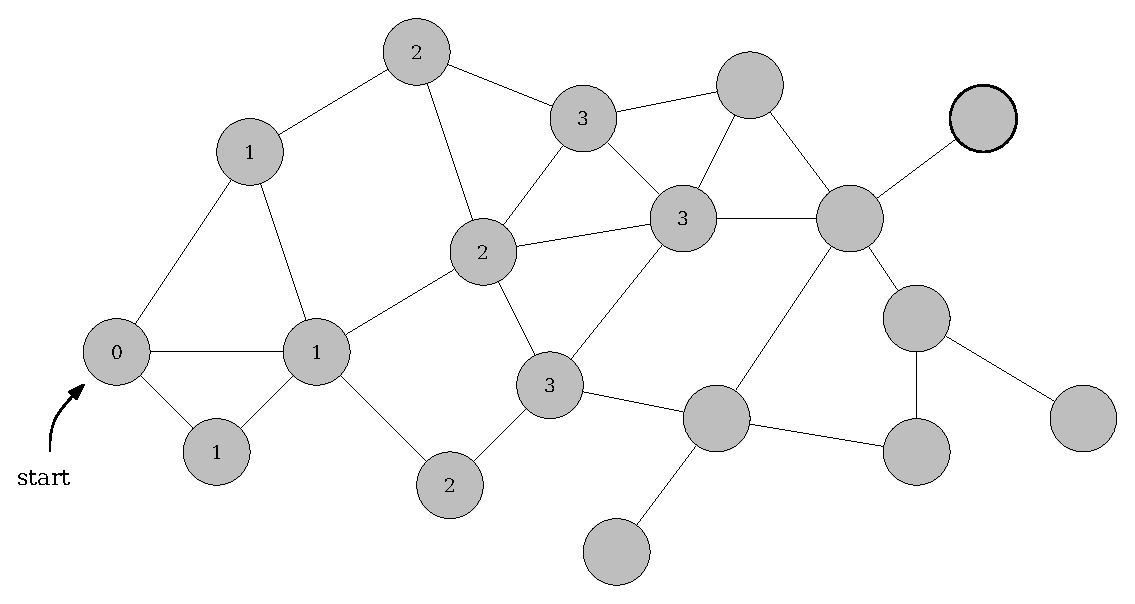
\includegraphics[width=0.6\textwidth]{./algorithms/breadth-first-search/partial-bfs}
	\caption{\small A partially completed breadth-first search on a graph with no particular target node.}
\end{figure}

\subsection{Applications}

\begin{itemize}
	\item Searching graphs with unit edges.
		Graphs with weighted edges should use the Dijkstra or Floyd-Warshall algorithm.
	\item Finding the shortest path between two given nodes.
	\item Testing a given graph for bipartiteness.
	By applying arbitrary, alternating labels to nodes as they are visited, one can determine if a graph is bipartite if a break in the alternation occurs.
\end{itemize}

\subsection{Example Contest Problem: Hopping Stones}

Contemplating wave-based trigonometric functions down by the river forming the southern edge of Farmer John's property may have kept the cows busy for a little while, but studying cowculus with their mathematics mentors is still on their mind.
They must escape the bounds of the fences.
The problem is that not all of them are able to hop the fence, and none would desire to destroy Farmer John's hard work.

There are a number of large rocks in the river that the cows could use to go around the edge of the fencing.
However, many of the cows are queasy about being over the deep waters that it holds and would rather hop around as little as possible.

Reassure the hesitating cows by finding the length of the shortest route possible for them to cross.

\subsubsection{Input}
\begin{itemize}
	\item Line 1: An unsigned integer representing the starting position of the cows.
	\item Line 2: An unsigned integer representing the number of the destination to be hopped to.
	\item Line 3 to EOF: A pair of unsigned integers representing the stones that can be hopped between.
\end{itemize}

\subsubsection{Sample Input}
\acmlisting[label=Hopping Stones Input, caption=Hopping Stones Input]{./algorithms/breadth-first-search/problems/hopping-stones/hopping-stones.in}

\subsubsection{Output}
Text formatted as in the sample output stating the number of hops that must be made to reach the specified destination.

\subsubsection{Sample Output}
\acmlisting[label=Hopping Stones Output, caption=Hopping Stones Output]{./algorithms/breadth-first-search/problems/hopping-stones/hopping-stones.out}

\subsubsection{Example Solution}
\acmlisting[label=Hopping Stones Solution, caption=Hopping Stones Solution]{./algorithms/breadth-first-search/problems/hopping-stones/hopping-stones.cpp}

\subsubsection{Lessons Learned}
\begin{itemize}
	\item If no target node is specified, the algorithm will completely propogate to all reachable nodes.
		This will result in shortest path calculation for all nodes.
	\item Representing the edges as a pair of unsigned integers is much quicker than using a dedicated struct.
\end{itemize}

\subsection{ACM Contest Problem: Word Ladder\cite{acmsoutheastregional2014}}
A \textit{word ladder} is a puzzle in which you transform one word into another by changing one letter at a time.
But, there's a catch: every word that you form in each step must be in the dictionary!
Here's an example of how to transform \textbf{CAT} into \textbf{GAS}:

\vspace{0.15in}

\begin{center}
\textbf{CAT} $\to$ \textbf{CAR} $\to$ \textbf{WAR} $\to$ \textbf{WAS} $\to$ \textbf{GAS}
\end{center}

\vspace{0.15in}

Of course, you want to use the fewest number of transitions possible.
These puzzles can be tough, and often you'll think to yourself:
''Darn it! If only $[$\textit{some word}$]$ was in the dictionary!''

Well, now is your chance!
Given a dictionary, and a starting and ending word, what ONE single word could you add to the dictionary to minimize the number of steps to get from the starting word to the ending word, changing one letter at a time, and making sure that every word at every step is in the dictionary?

\subsubsection{Input}
Each input will consist of a single test case.
Note that your program may be run multiple times on different inputs.
Each test case will start with a line with a single integer $n$ $(2 \le n \le 1000)$ which indicates the number of words in the dictionary.
The dictionary will follow on the next $n$ lines , with one word per line.
All words will consist of between 1 and 8 capital letters only, and all words in a test case wil be the same length.
The first word in the list will be the starting word of the word ladder, and the second word will be the ending word of the word ladder.

\subsubsection{Output}
Output exactly two lines.
The first line holds the one single word that you would add to the dictionary, and the second holds an integer indicating the minimum number of steps to get from the starting word to the ending word, adding your word. Output no spaces.

It is possible that there's more than one word you can add that will make your path as short as possible.
In this case, output the solution word that comes first alphabetically.

It is possible that there's no word you can add that makes the solution possible.
In this case, output $0$ (zero) as the word, and $-1$ as the number of steps.

\section{Depth-first Search}
\index{depth-first search}
\index{search!depth-first}
\index{DFS}

Depth-first search is a method of searching a graph for the possibility reaching a specified node.
As its name suggests, the algorithm will proceed from the starting node to the farthest node of a graph before branching to other nodes.
Because of this, depth-first search is \textbf{not} guaranteed to find the shortest path.
Rather, it will find \textbf{a} path if it exists.
Traversing an entire graph takes $\Theta (m + n)$ for a graph of $m$ vertices and $n$ edges.

\subsection{Applications}
\begin{itemize}
	\item Testing if two graphs are connected by some common node.
	\item Discovering whether a specified state is possible with certain steps.
	\item Finding connected and strongly connected components in $O(m + n)$ time.
\end{itemize}

\subsection{Example Contest Problem: Shaky Stones}
For a while now, the cows have been circumventing the new fence Farmer John built by traversing large rocks that are embedded in the river by the farm.
Some of the stones have become unstable after the cows have used them a number of times.
The ones that are likely to move or sink away have been pointed out by the perceptive cows and given an estimate of the number of times left the stones can be used.

Once again, it's time for the cows to meet their mathematics mentors, and, to do so this time, they need to use the large rocks to get around the fencing.
The cows know which rocks should not be used after a number of times.

Inform the cows of whether they'll all be able to make it, or whether a few need will need to stay behind and be tutored later.

\subsubsection{Input}
\begin{itemize}
	\item Line 1: The number of cows needing to cross.
	\item Line 2: The number of stones that can be used for crossing.
	\item Line 3: The assigned number of the stone the cows start at.
	\item Line 4: The assigned number of the stone the cows finish at.
	\item Line 5: The number of stones, $r$, that have restrictions on them.
	\item Line 6 to $6 + r - 1$: Two integers, the first representing the assigned number of the stone with the restriction on it, and the second representing the number of hops that are deemed safe for it.
	\item Line $6 + r$ to EOF: Two integers representing stones that can be safely hopped between.
\end{itemize}

\subsubsection{Sample Input}
\acmlisting[label=Shaky Stones Input, caption=Shaky Stones Input]{./algorithms/depth-first-search/problems/shaky-stones/shaky-stones.in}

\subsubsection{Output}
\begin{itemize}
	\item Line 1: Print the text 'It is possible.' followed by a newline if the specified number of cows can cross.
		Otherwise, print the text 'It is not possible. Only $x$ can cross' where $x$ is the number of cows that can cross.
\end{itemize}

\subsubsection{Sample Output}
\acmlisting[label=Shaky Stones Output, caption=Shaky Stones Output]{./algorithms/depth-first-search/problems/shaky-stones/shaky-stones.out}

\subsubsection{Example Solution}
\acmlisting[label=Shaky Stones Solution, caption=Shaky Stones Solution]{./algorithms/depth-first-search/problems/shaky-stones/shaky-stones.cpp}

\subsubsection{Lessons Learned}
\begin{itemize}
	\item Depth-first search could also be implemented using a stack in place of where breadth-first search would use a queue.
	\item The algorithm can be written using a while-loop instead of recursion.
\end{itemize}


\chapter{Approaches}
\section{Hash Window Approaches}\index{hashing}\index{hash windows}
Hashing is a mapping of objects to bytes.
These bytes are often stored in Strings or numeric data types.
Normally, hash functions attempt to map each object to a \textit{unique} set of bytes.
Also a \textit{slight} change in the object should cause a \textit{large} change in the output.
When two objects map to the same set of bytes, it is referred to as a hash collision.

\subsection{Approaches}
\begin{itemize}
	\item Identify substrings quickly and cleanly.
	\item Hash collisions to detect certain features of the input.
\end{itemize}

\subsection{Fine Print Returns!}
The cows have prepared another legal document for Farmer John to review.

The Cows are still championing the installation of an Olympic style swimming pool.
However, this time Farmer John only cares about how many times, `pool' appears in the text.

Help Farmer John determine how many times the text `pool' appears in the document.

\subsubsection{Input}
\begin{itemize}
	\item A stream of text terminated by an EOF representing the legal agreement
\end{itemize}

\subsubsection{Sample Input}
\acmlisting[label=Fine Print Sample Input, caption=Fine Print Sample Input]{./approaches/hashing/problems/fine-print/fine-print.in}

\subsubsection{Output}
\begin{itemize}
	\item 1 integer representing the number of references to the word pool in the text.
\end{itemize}

\subsubsection{Sample Output}
\acmlisting[label=Fine Print Sample Output, caption=Fine Print Sample Output]{./approaches/hashing/problems/fine-print/fine-print.out}

\subsubsection{Sample Solution}
\acmlisting[label=Fine Print Sample Solution, caption=Fine Print Sample Solution]{./approaches/hashing/problems/fine-print/fine-print.cpp}

\subsubsection{Lessons Learned}
\begin{itemize}
	\item There is often more than one way to solve a problem,  checkout the KMP string matching algorithm for another way to solve this problem.
\end{itemize}

\section{Dynamic Programming}\index{Dynamic Programming}
Dynamic Programming is a powerful tool that can be applied to several different types of algorithms.\cite{dppractice}
The basic idea is to save the results of smaller problems and use the results to solve larger problems.

\subsection{Applications}
\begin{itemize}
	\item	Improving runtimes of some other algorithms
	\item	Solving the knapsack in $O(nm)$ time
	\item	Solving the integer knapsack in $O(nm)$ time
	\item	Solving the largest increasing subsequence in $O(n \log n)$ time
	\item	Solving the maximum value sub-array problem in $O(n)$
	\item	Solving the maximum value continuous sub-array problem
\end{itemize}

\subsection{Example Contest Problem: A Knapsack Full of Fireworks}\index{Knapsack}
The cows on Farmer John's Farm are planning on putting on a fireworks show for Farmer John's birthday.

They have pooled all of their loose change, and hope to purchase a collection of fireworks that will maximize  Farmer John's amazement during the show so that he will be more likely to build them a new barn.
Each firework's label helpfully includes a "wow factor" rating explicitly for this purpose.
A high "wow factor" is more desirable than a low one.

Please help the cows determine the maximum "wow factor" they can get for their loose change.

\subsubsection{Input Format}
\begin{itemize}
	\item Line 1: One integer, $N$ $(1 \leq N \leq 100)$, the number of fireworks in the catalog.
   \item Line 2: One integer, $C$ $(1 \leq C \leq 10000)$, the total amount of change that the cows have to spend.
	\item Lines 3..$(N+2)$ Two integers $P,W$ representing the price and wow factor for the fireworks.
\end{itemize}

\subsubsection{Sample Input}
\acmlisting[caption=A Knapsack Full of Fireworks Input, label=A Knapsack Full of Fireworks Input]{./approaches/dp/problems/knapsack/knapsack.in}

\subsubsection{Output Format}
\begin{itemize}
	\item Line 1: A single integer representing the maximum wow factor.
\end{itemize}
\subsubsection{Sample Output}
\acmlisting[caption=A Knapsack Full of Fireworks Output, label=A Knapsack Full of Fireworks Output]{./approaches/dp/problems/knapsack/knapsack.out}

\subsubsection{Example Solution}
\acmlisting[caption=A Knapsack Full of Fireworks Solution, label=A Knapsack Full of Fireworks Solution]{./approaches/dp/problems/knapsack/knapsack.cpp}

\subsubsection{Lessons Learned}
The optimal solution is of the form:
$$W(j) = \max \left\{W(j-1), \max \left\{W(j - p_i) + v_i \right\}\right\}$$
Where $W(0) = 0$

\subsection{Example Contest Problem: A Few Fireworks More}\index{Knapsack!Integer}
The cows have reconsidered their original plan of buying just the fireworks with the greatest total "wow factor".
Instead, they want to incorporate "wow factor" \emph{and} diversity, so the cows have decided to purchase a collection of fireworks that optimizes "wow factor" and includes no more than one of each kind of firework in the catalog.

Please help the cows determine the maximum "wow factor" they can get for their loose change, on the condition that they purchase no more than one of each kind of firework in the catalog.

\subsubsection{Input}
\begin{itemize}
	\item Line 1: One integer, $N$, $(1 \leq N \leq 100)$ the number of fireworks in the catalog.
	\item Line 2: One integer, $C$, $(1 \leq C \leq 10000)$ the number of cents that the cows found.
	\item Lines 3..$(N+2)$ Two integers $P,W$ representing the price and wow factor for the fireworks.
\end{itemize}

\subsubsection{Sample Input}
\acmlisting[caption=A Few Fireworks More Input, label=A Few Fireworks More Input]{./approaches/dp/problems/one-zero/one-zero.in}

\subsubsection{Output Format}
\begin{itemize}
	\item Line 1: A single integer representing the maximum wow factor using each firework at most once
\end{itemize}
\subsubsection{Sample Output}
\acmlisting[caption=A Few Fireworks More Output, label=A Few Fireworks More Output]{./approaches/dp/problems/one-zero/one-zero.out}

\subsubsection{Example Solution}
\acmlisting[caption=A Few Fireworks More Solution, label=A Few Fireworks More Solution]{./approaches/dp/problems/one-zero/one-zero.cpp}

\subsubsection{Lesson Learned}
A similar problem to the knapsack, except each item can be used at most once.  The solution here is to expand the state space.  The optimal solution is of the form
$$M(i,j) = \max \left\{ M(i-1, j) , M(i-1, j- s_i) + v_i \right\}$$
Where $M(0,j) = 0$ and $M(i,0) = 0$

\subsection{Example Contest Problem: The Good, the Bad, the Cowy}\index{Largest Increasing Subsequence}
Farmer John's birthday party went off without a hitch, but the cows are worried that Farmer John isn't yet convinced that he should build the cows a new barn. Just in case, they have decided to put it to a vote whether or not they should bake him a cake as well.
Unfortunately, the cows are all experts in the school of bovine politics, and think that a simple majority vote will simply not do because of the dangers of vote rigging.

Instead, the cows have resorted to a rather odd voting system: each cow votes in some arbitrary order with an integer value, and if the length of largest increasing subsequence of all the votes is greater than half the number of cows, then the cows will bake Farmer John a cake.

Help the cows determine the results of their vote.

\subsubsection{Input}
\begin{itemize}
	\item Line 1: Several integers, separated by spaces, representing the votes of the cows.
\end{itemize}

\subsubsection{Sample Input}
\acmlisting[caption={The Good, the Bad, the Cowy Input}, label={The Good, the Bad, the Cowy Input}]{./approaches/dp/problems/cowy/cowy.in}

\subsubsection{Output Format}
\begin{itemize}
	\item Line 1: ``1'' if the cows have decided to bake a cake, and ``0'' otherwise.
\end{itemize}
\subsubsection{Sample Output}
\acmlisting[caption={The Good, the Bad, the Cowy Output}, label={The Good, the Bad, the Cowy Output}]{./approaches/dp/problems/cowy/cowy.out}

\subsubsection{Example Solution}
\acmlisting[caption={The Good, the Bad, the Cowy Solution}, label={The Good, the Bad, the Cowy Solution}]{./approaches/dp/problems/cowy/cowy.cpp}

\subsubsection{Lesson Learned}
\begin{itemize}
	\item This problem can be solved in $O(n \log n)$ time.
	\item Sometimes you have to check the entire array to find the solution.
	\item $while(cin >> val)$ can be used to read in an uncertain number of values.
\end{itemize}


\chapter{Appendix}
\section{C IO Functions}
Occasionally it is far easier to use the C IO functions to meet an output spec. It is also possible to set the precision and width options via numbers after the present,but before the specifier.  The general form of a specifier is: 

\begin{lstlisting}[label=format code format,caption=Format Codes for printf()]
%[flags][width][.precision][length]specifier
\end{lstlisting}

\begin{table}[h]
	\caption{Format Specifier Codes\cite{cplusplus}}
	\begin{tabularx}{\textwidth}{|l|X|l|} \hline
		Format Code &   Output              &   Example     \\ \hline
		d           &   Signed Int          &   314         \\
		u           &   Unsigned Int        &   314         \\
		o           &   Unsigned Octal      &   472         \\
		x           &   Unsigned hex        &   13a         \\
		X           &   UNSIGNED HEX        &   13A         \\
		f           &   floating point      &   3.140000    \\
		e           &   Scientific notation &   3.140000e+00\\
		c           &   character           &   A           \\
		s           &   string              &   ACM         \\
		p           &   pointer address     &   0x40060c    \\
		l           &   Used with other specifiers to indicate a long & 314 \\
		\%\%        &   Prints a literal \% &   \%          \\
		\hline
	\end{tabularx}
\end{table}

\begin{table}[h]
	\caption{Modifier Flags \cite{cplusplus}}
	\begin{tabularx}{\textwidth}{|l|X|l|} \hline
		Format Code &   Output                  &   Example    \\ \hline
		-           &   Left-justify            &   314        \\
		+           &   Force-sign character    &   +314       \\
		\#          &   Show prefix             &   0x13a      \\
			  &   Show decimal point      &   314.       \\
		0           &   Left pad field with 0   &   0314       \\
		\hline
	\end{tabularx}
\end{table}

\subsection{Examples}
\acmlisting[language=c++]{./general/ciofunctions/ciofunctions.cpp}

\section{Some Basic VIMRC Settings}
\acmlisting[language={}, label=vimrc,caption=vimrc]{./general/vimrc/vimrc.example}

\section{Makefile}
\acmlisting[language={}, label=makefile, caption=makefile]{./general/makefile/makefile.example}


#ifdef hackpackpp
\chapter{C++ Standard Library}
This chapter was pulled from cppreference.com\cite{cppreference}.
\section{Utilities library}

\subsection{std::pair}

\subsubsection{NAME}
std::pair - std::pair is a struct template that provides a way to store two heterogeneous objects as a single unit. A pair is a specific case of a std::tuple with two elements.

\subsubsection{SYNOPSIS}
\#include <utility>

\begin{lstlisting}
 template<
    class T1,
    class T2
> struct pair;
\end{lstlisting}

\subsubsection{MEMBER FUNCTIONS}
std::pair::pair(3) - constructs new pair  (public member function)
std::pair::operator=(3) - assigns the contents  (public member function)
std::pair::swap(3) [C++11] - swaps the contents   (public member function)

\subsubsection{NON-MEMBER FUNCTIONS}
make\_pair(3) - creates a pair object of type, defined by the argument types  (function template)
operator==(3), operator!=(3), operator<(3), operator<=(3), operator>(3), operator>=(3) - lexicographically compares the values in the pair   (function template)
std::swap(std::pair)(3) [C++11] - specializes the std::swap algorithm   (function template)
std::get(std::pair)(3) [C++11] - accesses an element of a pair   (function template)


\subsection{std::tuple}

\subsubsection{NAME}
std::tuple - Class template std::tuple is a fixed-size collection of heterogeneous values. It is a generalization of std::pair.

\subsubsection{SYNOPSIS}
\#include <tuple>

\begin{lstlisting}
 template< class... Types >
class tuple; [since C++11]
\end{lstlisting}

\subsubsection{MEMBER FUNCTIONS}
std::tuple::tuple(3) - constructs a new tuple  (public member function)
std::tuple::operator=(3) - assigns the contents of one tuple to another  (public member function)
std::tuple::swap(3) - swaps the contents of two tuples   (public member function)

\subsubsection{NON-MEMBER FUNCTIONS}
make\_tuple(3) - creates a tuple object of the type defined by the argument types  (function template)
tie(3) - creates a tuple of lvalue references or unpacks a tuple into individual objects  (function template)
forward\_as\_tuple(3) - creates a tuple of rvalue references  (function template)
tuple\_cat(3) - creates a tuple by concatenating any number of tuples  (function template)
std::get(std::tuple)(3) - tuple accesses specified element  (function template)
operator==(3), operator!=(3), operator<(3), operator<=(3), operator>(3), operator>=(3) - lexicographically compares the values in the tuple   (function template)
std::swap(std::tuple)(3) [C++11] - specializes the std::swap algorithm   (function template)


\section{Strings library}

\subsection{std::basic\_string}

\subsubsection{NAME}
std::basic\_string - The class template basic\_string stores and manipulates sequences of char-like objects. The class is dependent neither on the character type nor on the nature of operations on that type. The definitions of the operations are supplied via the Traits template parameter - a specialization of std::char\_traits or a compatible traits class.

\subsubsection{SYNOPSIS}
\#include <string>

\begin{lstlisting}
 template<
    class CharT,
    class Traits = std::char\_traits<CharT>,
    class Allocator = std::allocator<CharT>
> class basic\_string;
\end{lstlisting}

\subsubsection{MEMBER FUNCTIONS}
std::basic\_string::basic\_string(3) - constructs a basic\_string  (public member function)
std::basic\_string::operator=(3) - assigns values to the string   (public member function)
std::basic\_string::assign(3) - assign characters to a string  (public member function)
std::basic\_string::get\_allocator(3) - returns the associated allocator   (public member function)
\paragraph{Element access}
std::basic\_string::at(3) - access specified character with bounds checking  (public member function)
std::basic\_string::operator[](3) - access specified character  (public member function)
std::basic\_string::front(3) [C++11] - accesses the first character  (public member function)
std::basic\_string::back(3) [C++11] - accesses the last character  (public member function)
std::basic\_string::data(3) - returns a pointer to the first character of a string  (public member function)
std::basic\_string::c\_str(3) - returns a non-modifiable standard C character array version of the string  (public member function)
\paragraph{Iterators}
std::basic\_string::begin(3), std::basic\_string::cbegin(3) [C++11] - returns an iterator to the beginning   (public member function)
std::basic\_string::end(3), std::basic\_string::cend(3) [C++11] - returns an iterator to the end   (public member function)
std::basic\_string::rbegin(3), std::basic\_string::crbegin(3) [C++11] - returns a reverse iterator to the beginning   (public member function)
std::basic\_string::rend(3), std::basic\_string::crend(3) [C++11] - returns a reverse iterator to the end   (public member function)
\paragraph{Capacity}
std::basic\_string::empty(3) - checks whether the string is empty   (public member function)
std::basic\_string::size(3), std::basic\_string::length(3) - returns the number of characters   (public member function)
std::basic\_string::max\_size(3) - returns the maximum number of characters   (public member function)
std::basic\_string::reserve(3) - reserves storage   (public member function)
std::basic\_string::capacity(3) - returns the number of characters that can be held in currently allocated storage   (public member function)
std::basic\_string::shrink\_to\_fit(3) [C++11] - reduces memory usage by freeing unused memory   (public member function)
\paragraph{Operations}
std::basic\_string::clear(3) - clears the contents  (public member function)
std::basic\_string::insert(3) - inserts characters  (public member function)
std::basic\_string::erase(3) - removes characters   (public member function)
std::basic\_string::push\_back(3) - appends a character to the end  (public member function)
std::basic\_string::pop\_back(3) [C++11] - removes the last character   (public member function)
std::basic\_string::append(3) - appends characters to the end  (public member function)
std::basic\_string::operator+=(3) - appends characters to the end  (public member function)
std::basic\_string::compare(3) - compares two strings  (public member function)
std::basic\_string::replace(3) - replaces specified portion of a string  (public member function)
std::basic\_string::substr(3) - returns a substring  (public member function)
std::basic\_string::copy(3) - copies characters  (public member function)
std::basic\_string::resize(3) - changes the number of characters stored   (public member function)
std::basic\_string::swap(3) - swaps the contents   (public member function)
\paragraph{Search}
std::basic\_string::find(3) - find characters in the string  (public member function)
std::basic\_string::rfind(3) - find the last occurrence of a substring  (public member function)
std::basic\_string::find\_first\_of(3) - find first occurrence of characters  (public member function)
std::basic\_string::find\_first\_not\_of(3) - find first absence of characters  (public member function)
std::basic\_string::find\_last\_of(3) - find last occurrence of characters  (public member function)
std::basic\_string::find\_last\_not\_of(3) - find last absence of characters  (public member function)

\subsubsection{NON-MEMBER FUNCTIONS}
operator+(3) - concatenates two strings or a string and a char   (function template)
operator==(3), operator!=(3), operator<(3), operator>(3), operator<=(3), operator>=(3) - lexicographically compares two strings   (function template)
std::swap(std::basic\_string)(3) - specializes the std::swap algorithm  (function template)
\paragraph{Input/output}
operator<<(3), operator>>(3) - performs stream input and output on strings   (function template)
getline(3) - read data from an I/O stream into a string  (function)
\paragraph{Numeric conversions}
stoi(3), stol(3), stoll [C++11] [C++11](3) [C++11] - converts a string to a signed integer   (function)
stoul(3), stoull [C++11](3) [C++11] - converts a string to an unsigned integer   (function)
stof(3), stod(3), stold [C++11] [C++11](3) [C++11] - converts a string to a floating point value   (function)
to\_string(3) [C++11] - converts an integral or floating point value to string   (function)
to\_wstring(3) [C++11] - converts an integral or floating point value to wstring   (function)


\section{Containers library}

\subsection{std::array}

\subsubsection{NAME}
std::array - std::array is a container that encapsulates fixed size arrays.

\subsubsection{SYNOPSIS}
\#include <array>

\begin{lstlisting}
 template<
    class T,
    std::size\_t N

> struct array; [since C++11]
\end{lstlisting}

\subsubsection{MEMBER FUNCTIONS}
\paragraph{Implicitly-defined member functions}
std::array::array(implicitly declared)(3) - default-initializes or copy-initializes every element of the array  (public member function)
std::array::~array(implicitly declared)(3) - destroys every element of the array  (public member function)
std::array::operator=(implicitly declared)(3) - overwrites every element of the array with the corresponding element of another array  (public member function)
\paragraph{Element access}
std::array::at(3) - access specified element with bounds checking   (public member function)
std::array::operator[](3) - access specified element   (public member function)
std::array::front(3) - access the first element   (public member function)
std::array::back(3) - access the last element   (public member function)
std::array::data(3) - direct access to the underlying array   (public member function)
\paragraph{Iterators}
std::array::begin(3), std::array::cbegin(3) - returns an iterator to the beginning   (public member function)
std::array::end(3), std::array::cend(3) - returns an iterator to the end   (public member function)
std::array::rbegin(3), std::array::crbegin(3) - returns a reverse iterator to the beginning   (public member function)
std::array::rend(3), std::array::crend(3) - returns a reverse iterator to the end   (public member function)
\paragraph{Capacity}
std::array::empty(3) - checks whether the container is empty   (public member function)
std::array::size(3) - returns the number of elements   (public member function)
std::array::max\_size(3) - returns the maximum possible number of elements   (public member function)
\paragraph{Operations}
std::array::fill(3) - fill the container with specified value   (public member function)
std::array::swap(3) - swaps the contents   (public member function)

\subsubsection{NON-MEMBER FUNCTIONS}
operator==(3), operator!=(3), operator<(3), operator<=(3), operator>(3), operator>=(3) - lexicographically compares the values in the array   (function template)
std::get(std::array)(3) - accesses an element of an array   (function template)
std::swap(std::array)(3) [C++11] - specializes the std::swap algorithm   (function template)


\subsection{std::vector}

\subsubsection{NAME}
std::vector - std::vector is a sequence container that encapsulates dynamic size arrays.

\subsubsection{SYNOPSIS}
\#include <vector>

\begin{lstlisting}
 template<
    class T,
    class Allocator = std::allocator<T>
> class vector;
\end{lstlisting}

\subsubsection{MEMBER FUNCTIONS}
std::vector::vector(3) - constructs the vector  (public member function)
std::vector::~vector(3) - destructs the vector  (public member function)
std::vector::operator=(3) - assigns values to the container   (public member function)
std::vector::assign(3) - assigns values to the container   (public member function)
std::vector::get\_allocator(3) - returns the associated allocator   (public member function)
\paragraph{Element access}
std::vector::at(3) - access specified element with bounds checking   (public member function)
std::vector::operator[](3) - access specified element   (public member function)
std::vector::front(3) - access the first element   (public member function)
std::vector::back(3) - access the last element   (public member function)
std::vector::data(3) [C++11] - direct access to the underlying array   (public member function)
\paragraph{Iterators}
std::vector::begin(3), std::vector::cbegin(3) - returns an iterator to the beginning   (public member function)
std::vector::end(3), std::vector::cend(3) - returns an iterator to the end   (public member function)
std::vector::rbegin(3), std::vector::crbegin(3) - returns a reverse iterator to the beginning   (public member function)
std::vector::rend(3), std::vector::crend(3) - returns a reverse iterator to the end   (public member function)
\paragraph{Capacity}
std::vector::empty(3) - checks whether the container is empty   (public member function)
std::vector::size(3) - returns the number of elements   (public member function)
std::vector::max\_size(3) - returns the maximum possible number of elements   (public member function)
std::vector::reserve(3) - reserves storage  (public member function)
std::vector::capacity(3) - returns the number of elements that can be held in currently allocated storage   (public member function)
std::vector::shrink\_to\_fit(3) [C++11] - reduces memory usage by freeing unused memory   (public member function)
\paragraph{Modifiers}
std::vector::clear(3) - clears the contents   (public member function)
std::vector::insert(3) - inserts elements   (public member function)
std::vector::emplace(3) [C++11] - constructs element in-place   (public member function)
std::vector::erase(3) - erases elements   (public member function)
std::vector::push\_back(3) - adds elements to the end  (public member function)
std::vector::emplace\_back(3) [C++11] - constructs elements in-place at the end   (public member function)
std::vector::pop\_back(3) - removes the last element   (public member function)
std::vector::resize(3) - changes the number of elements stored   (public member function)
std::vector::swap(3) - swaps the contents   (public member function)

\subsubsection{NON-MEMBER FUNCTIONS}
operator==(3), operator!=(3), operator<(3), operator<=(3), operator>(3), operator>=(3) - lexicographically compares the values in the vector   (function template)
std::swap(std::vector)(3) - specializes the std::swap algorithm   (function template)


\subsection{std::deque}

\subsubsection{NAME}
std::deque - std::deque (double-ended queue) is an indexed sequence container that allows fast insertion and deletion at both its beginning and its end. In addition, insertion and deletion at either end of a deque never invalidates pointers or references to the rest of the elements.

\subsubsection{SYNOPSIS}
\#include <deque>

\begin{lstlisting}
 template<
    class T,
    class Allocator = std::allocator<T>
> class deque;
\end{lstlisting}

\subsubsection{MEMBER FUNCTIONS}
std::deque::deque(3) - constructs the deque  (public member function)
std::deque::~deque(3) - destructs the deque  (public member function)
std::deque::operator=(3) - assigns values to the container   (public member function)
std::deque::assign(3) - assigns values to the container   (public member function)
std::deque::get\_allocator(3) - returns the associated allocator   (public member function)
\paragraph{Element access}
std::deque::at(3) - access specified element with bounds checking   (public member function)
std::deque::operator[](3) - access specified element   (public member function)
std::deque::front(3) - access the first element   (public member function)
std::deque::back(3) - access the last element   (public member function)
\paragraph{Iterators}
std::deque::begin(3), std::deque::cbegin(3) - returns an iterator to the beginning   (public member function)
std::deque::end(3), std::deque::cend(3) - returns an iterator to the end   (public member function)
std::deque::rbegin(3), std::deque::crbegin(3) - returns a reverse iterator to the beginning   (public member function)
std::deque::rend(3), std::deque::crend(3) - returns a reverse iterator to the end   (public member function)
\paragraph{Capacity}
std::deque::empty(3) - checks whether the container is empty   (public member function)
std::deque::size(3) - returns the number of elements   (public member function)
std::deque::max\_size(3) - returns the maximum possible number of elements   (public member function)
std::deque::shrink\_to\_fit(3) [C++11] - reduces memory usage by freeing unused memory   (public member function)
\paragraph{Modifiers}
std::deque::clear(3) - clears the contents   (public member function)
std::deque::insert(3) - inserts elements   (public member function)
std::deque::emplace(3) [C++11] - constructs element in-place   (public member function)
std::deque::erase(3) - erases elements   (public member function)
std::deque::push\_back(3) - adds elements to the end  (public member function)
std::deque::emplace\_back(3) [C++11] - constructs elements in-place at the end   (public member function)
std::deque::pop\_back(3) - removes the last element   (public member function)
std::deque::push\_front(3) - inserts elements to the beginning  (public member function)
std::deque::emplace\_front(3) [C++11] - constructs elements in-place at the beginning   (public member function)
std::deque::pop\_front(3) - removes the first element   (public member function)
std::deque::resize(3) - changes the number of elements stored   (public member function)
std::deque::swap(3) - swaps the contents   (public member function)

\subsubsection{NON-MEMBER FUNCTIONS}
operator==(3), operator!=(3), operator<(3), operator<=(3), operator>(3), operator>=(3) - lexicographically compares the values in the deque   (function template)
std::swap(std::deque)(3) - specializes the std::swap algorithm   (function template)


\subsection{std::forward\_list}

\subsubsection{NAME}
std::forward\_list - std::forward\_list is a container that supports fast insertion and removal of elements from anywhere in the container. Fast random access is not supported. It is implemented as a singly-linked list and essentially does not have any overhead compared to its implementation in C. Compared to std::list this container provides more space efficient storage when bidirectional iteration is not needed.

\subsubsection{SYNOPSIS}
\#include <forward\_list>

\begin{lstlisting}
 template<
    class T,
    class Allocator = std::allocator<T>

> class forward\_list; [since C++11]
\end{lstlisting}

\subsubsection{MEMBER FUNCTIONS}
std::forward\_list::forward\_list(3) - constructs the forward\_list  (public member function)
std::forward\_list::~forward\_list(3) - destructs the forward\_list  (public member function)
std::forward\_list::operator=(3) - assigns values to the container   (public member function)
std::forward\_list::assign(3) - assigns values to the container   (public member function)
std::forward\_list::get\_allocator(3) - returns the associated allocator   (public member function)
\paragraph{Element access}
std::forward\_list::front(3) - access the first element   (public member function)
\paragraph{Iterators}
std::forward\_list::before\_begin(3), std::forward\_list::cbefore\_begin(3) - returns an iterator to the element before beginning   (public member function)
std::forward\_list::begin(3), std::forward\_list::cbegin(3) - returns an iterator to the beginning   (public member function)
std::forward\_list::end(3), std::forward\_list::cend(3) - returns an iterator to the end   (public member function)
\paragraph{Capacity}
std::forward\_list::empty(3) - checks whether the container is empty   (public member function)
std::forward\_list::max\_size(3) - returns the maximum possible number of elements   (public member function)
\paragraph{Modifiers}
std::forward\_list::clear(3) - clears the contents   (public member function)
std::forward\_list::insert\_after(3) - inserts elements after an element   (public member function)
std::forward\_list::emplace\_after(3) - constructs elements in-place after an element   (public member function)
std::forward\_list::erase\_after(3) - erases an element after an element   (public member function)
std::forward\_list::push\_front(3) - inserts elements to the beginning  (public member function)
std::forward\_list::emplace\_front(3) - constructs elements in-place at the beginning   (public member function)
std::forward\_list::pop\_front(3) - removes the first element   (public member function)
std::forward\_list::resize(3) - changes the number of elements stored   (public member function)
std::forward\_list::swap(3) - swaps the contents   (public member function)
\paragraph{Operations}
std::forward\_list::merge(3) - merges two sorted lists  (public member function)
std::forward\_list::splice\_after(3) - moves elements from another forward\_list   (public member function)
std::forward\_list::remove(3), std::forward\_list::remove\_if(3) - removes elements satisfying specific criteria  (public member function)
std::forward\_list::reverse(3) - reverses the order of the elements  (public member function)
std::forward\_list::unique(3) - removes consecutive duplicate elements  (public member function)
std::forward\_list::sort(3) - sorts the elements  (public member function)

\subsubsection{NON-MEMBER FUNCTIONS}
operator==(3), operator!=(3), operator<(3), operator<=(3), operator>(3), operator>=(3) - lexicographically compares the values in the forward\_list   (function template)
std::swap(std::forward\_list)(3) [C++11] - specializes the std::swap algorithm   (function template)


\subsection{std::list}

\subsubsection{NAME}
std::list - std::list is a container that supports constant time insertion and removal of elements from anywhere in the container. Fast random access is not supported. It is usually implemented as double-linked list. Compared to std::forward\_list this container provides bidirectional iteration capability while being less space efficient.

\subsubsection{SYNOPSIS}
\#include <list>

\begin{lstlisting}
 template<
    class T,
    class Allocator = std::allocator<T>
> class list;
\end{lstlisting}

\subsubsection{MEMBER FUNCTIONS}
std::list::list(3) - constructs the list  (public member function)
std::list::~list(3) - destructs the list  (public member function)
std::list::operator=(3) - assigns values to the container   (public member function)
std::list::assign(3) - assigns values to the container   (public member function)
std::list::get\_allocator(3) - returns the associated allocator   (public member function)
\paragraph{Element access}
std::list::front(3) - access the first element   (public member function)
std::list::back(3) - access the last element   (public member function)
\paragraph{Iterators}
std::list::begin(3), std::list::cbegin(3) - returns an iterator to the beginning   (public member function)
std::list::end(3), std::list::cend(3) - returns an iterator to the end   (public member function)
std::list::rbegin(3), std::list::crbegin(3) - returns a reverse iterator to the beginning   (public member function)
std::list::rend(3), std::list::crend(3) - returns a reverse iterator to the end   (public member function)
\paragraph{Capacity}
std::list::empty(3) - checks whether the container is empty   (public member function)
std::list::size(3) - returns the number of elements   (public member function)
std::list::max\_size(3) - returns the maximum possible number of elements   (public member function)
\paragraph{Modifiers}
std::list::clear(3) - clears the contents   (public member function)
std::list::insert(3) - inserts elements   (public member function)
std::list::emplace(3) [C++11] - constructs element in-place   (public member function)
std::list::erase(3) - erases elements   (public member function)
std::list::push\_back(3) - adds elements to the end  (public member function)
std::list::emplace\_back(3) [C++11] - constructs elements in-place at the end   (public member function)
std::list::pop\_back(3) - removes the last element   (public member function)
std::list::push\_front(3) - inserts elements to the beginning  (public member function)
std::list::emplace\_front(3) [C++11] - constructs elements in-place at the beginning   (public member function)
std::list::pop\_front(3) - removes the first element   (public member function)
std::list::resize(3) - changes the number of elements stored   (public member function)
std::list::swap(3) - swaps the contents   (public member function)
\paragraph{Operations}
std::list::merge(3) - merges two sorted lists  (public member function)
std::list::splice(3) - moves elements from another list   (public member function)
std::list::remove(3), std::list::remove\_if(3) - removes elements satisfying specific criteria  (public member function)
std::list::reverse(3) - reverses the order of the elements  (public member function)
std::list::unique(3) - removes consecutive duplicate elements  (public member function)
std::list::sort(3) - sorts the elements  (public member function)

\subsubsection{NON-MEMBER FUNCTIONS}
operator==(3), operator!=(3), operator<(3), operator<=(3), operator>(3), operator>=(3) - lexicographically compares the values in the list   (function template)
std::swap(std::list)(3) - specializes the std::swap algorithm   (function template)


\subsection{std::set}

\subsubsection{NAME}
std::set - std::set is an associative container that contains a sorted set of unique objects of type Key. Sorting is done using the key comparison function Compare. Search, removal, and insertion operations have logarithmic complexity. Sets are usually implemented as red-black trees.

\subsubsection{SYNOPSIS}
\#include <set>

\begin{lstlisting}
 template<
    class Key,
    class Compare = std::less<Key>,
    class Allocator = std::allocator<Key>
> class set;
\end{lstlisting}

\subsubsection{MEMBER FUNCTIONS}
std::set::set(3) - constructs the set  (public member function)
std::set::~set(3) - destructs the set  (public member function)
std::set::operator=(3) - assigns values to the container   (public member function)
std::set::get\_allocator(3) - returns the associated allocator   (public member function)
\paragraph{Iterators}
std::set::begin(3), std::set::cbegin(3) - returns an iterator to the beginning   (public member function)
std::set::end(3), std::set::cend(3) - returns an iterator to the end   (public member function)
std::set::rbegin(3), std::set::crbegin(3) - returns a reverse iterator to the beginning   (public member function)
std::set::rend(3), std::set::crend(3) - returns a reverse iterator to the end   (public member function)
\paragraph{Capacity}
std::set::empty(3) - checks whether the container is empty   (public member function)
std::set::size(3) - returns the number of elements   (public member function)
std::set::max\_size(3) - returns the maximum possible number of elements   (public member function)
\paragraph{Modifiers}
std::set::clear(3) - clears the contents   (public member function)
std::set::insert(3) - inserts elements   (public member function)
std::set::emplace(3) [C++11] - constructs element in-place   (public member function)
std::set::emplace\_hint(3) [C++11] - constructs elements in-place using a hint   (public member function)
std::set::erase(3) - erases elements   (public member function)
std::set::swap(3) - swaps the contents   (public member function)
\paragraph{Lookup}
std::set::count(3) - returns the number of elements matching specific key   (public member function)
std::set::find(3) - finds element with specific key  (public member function)
std::set::equal\_range(3) - returns range of elements matching a specific key  (public member function)
std::set::lower\_bound(3) - returns an iterator to the first element not less than the given key  (public member function)
std::set::upper\_bound(3) - returns an iterator to the first element greater than the given key  (public member function)
\paragraph{Observers}
std::set::key\_comp(3) - returns the function that compares keys  (public member function)
std::set::value\_comp(3) - returns the function that compares keys in objects of type value\_type  (public member function)

\subsubsection{NON-MEMBER FUNCTIONS}
operator==(3), operator!=(3), operator<(3), operator<=(3), operator>(3), operator>=(3) - lexicographically compares the values in the set   (function template)
std::swap(std::set)(3) - specializes the std::swap algorithm   (function template)


\subsection{std::map}

\subsubsection{NAME}
std::map - std::map is a sorted associative container that contains key-value pairs with unique keys. Keys are sorted by using the comparison function Compare.  Search, removal, and insertion operations have logarithmic complexity. Maps are usually implemented as red-black trees.

\subsubsection{SYNOPSIS}
\#include <map>

\begin{lstlisting}
 template<
    class Key,
    class T,
    class Compare = std::less<Key>,
    class Allocator = std::allocator<std::pair<const Key, T> >
> class map;
\end{lstlisting}

\subsubsection{MEMBER FUNCTIONS}
std::map::map(3) - constructs the map  (public member function)
std::map::~map(3) - destructs the map  (public member function)
std::map::operator=(3) - assigns values to the container   (public member function)
std::map::get\_allocator(3) - returns the associated allocator   (public member function)
\paragraph{Element access}
std::map::at(3) [C++11] - access specified element with bounds checking   (public member function)
std::map::operator[](3) - access specified element   (public member function)
\paragraph{Iterators}
std::map::begin(3), std::map::cbegin(3) - returns an iterator to the beginning   (public member function)
std::map::end(3), std::map::cend(3) - returns an iterator to the end   (public member function)
std::map::rbegin(3), std::map::crbegin(3) - returns a reverse iterator to the beginning   (public member function)
std::map::rend(3), std::map::crend(3) - returns a reverse iterator to the end   (public member function)
\paragraph{Capacity}
std::map::empty(3) - checks whether the container is empty   (public member function)
std::map::size(3) - returns the number of elements   (public member function)
std::map::max\_size(3) - returns the maximum possible number of elements   (public member function)
\paragraph{Modifiers}
std::map::clear(3) - clears the contents   (public member function)
std::map::insert(3) - inserts elements   (public member function)
std::map::insert\_or\_assign(3) [C++17] - inserts an element or assigns to the current element if the key already exists   (public member function)
std::map::emplace(3) [C++11] - constructs element in-place   (public member function)
std::map::emplace\_hint(3) [C++11] - constructs elements in-place using a hint   (public member function)
std::map::try\_emplace(3) [C++17] - inserts in-place if the key does not exist, does nothing if the key exists  (public member function)
std::map::erase(3) - erases elements   (public member function)
std::map::swap(3) - swaps the contents   (public member function)
\paragraph{Lookup}
std::map::count(3) - returns the number of elements matching specific key   (public member function)
std::map::find(3) - finds element with specific key  (public member function)
std::map::equal\_range(3) - returns range of elements matching a specific key  (public member function)
std::map::lower\_bound(3) - returns an iterator to the first element not less than the given key  (public member function)
std::map::upper\_bound(3) - returns an iterator to the first element greater than the given key  (public member function)
\paragraph{Observers}
std::map::key\_comp(3) - returns the function that compares keys  (public member function)
std::map::value\_comp(3) - returns the function that compares keys in objects of type value\_type  (public member function)

\subsubsection{NON-MEMBER FUNCTIONS}
operator==(3), operator!=(3), operator<(3), operator<=(3), operator>(3), operator>=(3) - lexicographically compares the values in the map   (function template)
std::swap(std::map)(3) - specializes the std::swap algorithm   (function template)


\subsection{std::multiset}

\subsubsection{NAME}
std::multiset - Multiset is an associative container that contains a sorted set of objects of type Key. Unlike set, multiple keys with equal values are allowed. Sorting is done using the key comparison function Compare. Search, insertion, and removal operations have logarithmic complexity.

\subsubsection{SYNOPSIS}
\#include <set>

\begin{lstlisting}
 template<
    class Key,
    class Compare = std::less<Key>,
    class Allocator = std::allocator<Key>
> class multiset;
\end{lstlisting}

\subsubsection{MEMBER FUNCTIONS}
std::multiset::multiset(3) - constructs the multiset  (public member function)
std::multiset::~multiset(3) - destructs the multiset  (public member function)
std::multiset::operator=(3) - assigns values to the container   (public member function)
std::multiset::get\_allocator(3) - returns the associated allocator   (public member function)
\paragraph{Iterators}
std::multiset::begin(3), std::multiset::cbegin(3) - returns an iterator to the beginning   (public member function)
std::multiset::end(3), std::multiset::cend(3) - returns an iterator to the end   (public member function)
std::multiset::rbegin(3), std::multiset::crbegin(3) - returns a reverse iterator to the beginning   (public member function)
std::multiset::rend(3), std::multiset::crend(3) - returns a reverse iterator to the end   (public member function)
\paragraph{Capacity}
std::multiset::empty(3) - checks whether the container is empty   (public member function)
std::multiset::size(3) - returns the number of elements   (public member function)
std::multiset::max\_size(3) - returns the maximum possible number of elements   (public member function)
\paragraph{Modifiers}
std::multiset::clear(3) - clears the contents   (public member function)
std::multiset::insert(3) - inserts elements   (public member function)
std::multiset::emplace(3) [C++11] - constructs element in-place   (public member function)
std::multiset::emplace\_hint(3) [C++11] - constructs elements in-place using a hint   (public member function)
std::multiset::erase(3) - erases elements   (public member function)
std::multiset::swap(3) - swaps the contents   (public member function)
\paragraph{Lookup}
std::multiset::count(3) - returns the number of elements matching specific key   (public member function)
std::multiset::find(3) - finds element with specific key  (public member function)
std::multiset::equal\_range(3) - returns range of elements matching a specific key  (public member function)
std::multiset::lower\_bound(3) - returns an iterator to the first element not less than the given key  (public member function)
std::multiset::upper\_bound(3) - returns an iterator to the first element greater than the given key  (public member function)
\paragraph{Observers}
std::multiset::key\_comp(3) - returns the function that compares keys  (public member function)
std::multiset::value\_comp(3) - returns the function that compares keys in objects of type value\_type  (public member function)

\subsubsection{NON-MEMBER FUNCTIONS}
operator==(3), operator!=(3), operator<(3), operator<=(3), operator>(3), operator>=(3) - lexicographically compares the values in the multiset   (function template)
std::swap(std::multiset)(3) - specializes the std::swap algorithm   (function template)


\subsection{std::multimap}

\subsubsection{NAME}
std::multimap - Multimap is an associative container that contains a sorted list of key-value pairs. Sorting is done according to the comparison function Compare, applied to the keys. Search, insertion, and removal operations have logarithmic complexity.

\subsubsection{SYNOPSIS}
\#include <map>

\begin{lstlisting}
 template<
    class Key,
    class T,
    class Compare = std::less<Key>,
    class Allocator = std::allocator<std::pair<const Key, T> >
> class multimap;
\end{lstlisting}

\subsubsection{MEMBER FUNCTIONS}
std::multimap::multimap(3) - constructs the multimap  (public member function)
std::multimap::~multimap(3) - destructs the multimap  (public member function)
std::multimap::operator=(3) - assigns values to the container   (public member function)
std::multimap::get\_allocator(3) - returns the associated allocator   (public member function)
\paragraph{Iterators}
std::multimap::begin(3), std::multimap::cbegin(3) - returns an iterator to the beginning   (public member function)
std::multimap::end(3), std::multimap::cend(3) - returns an iterator to the end   (public member function)
std::multimap::rbegin(3), std::multimap::crbegin(3) - returns a reverse iterator to the beginning   (public member function)
std::multimap::rend(3), std::multimap::crend(3) - returns a reverse iterator to the end   (public member function)
\paragraph{Capacity}
std::multimap::empty(3) - checks whether the container is empty   (public member function)
std::multimap::size(3) - returns the number of elements   (public member function)
std::multimap::max\_size(3) - returns the maximum possible number of elements   (public member function)
\paragraph{Modifiers}
std::multimap::clear(3) - clears the contents   (public member function)
std::multimap::insert(3) - inserts elements   (public member function)
std::multimap::emplace(3) [C++11] - constructs element in-place   (public member function)
std::multimap::emplace\_hint(3) [C++11] - constructs elements in-place using a hint   (public member function)
std::multimap::erase(3) - erases elements   (public member function)
std::multimap::swap(3) - swaps the contents   (public member function)
\paragraph{Lookup}
std::multimap::count(3) - returns the number of elements matching specific key   (public member function)
std::multimap::find(3) - finds element with specific key  (public member function)
std::multimap::equal\_range(3) - returns range of elements matching a specific key  (public member function)
std::multimap::lower\_bound(3) - returns an iterator to the first element not less than the given key  (public member function)
std::multimap::upper\_bound(3) - returns an iterator to the first element greater than the given key  (public member function)
\paragraph{Observers}
std::multimap::key\_comp(3) - returns the function that compares keys  (public member function)
std::multimap::value\_comp(3) - returns the function that compares keys in objects of type value\_type  (public member function)

\subsubsection{NON-MEMBER FUNCTIONS}
operator==(3), operator!=(3), operator<(3), operator<=(3), operator>(3), operator>=(3) - lexicographically compares the values in the multimap   (function template)
std::swap(std::multimap)(3) - specializes the std::swap algorithm   (function template)


\subsection{std::unordered\_set}

\subsubsection{NAME}
std::unordered\_set - Unordered set is an associative container that contains set of unique objects of type Key. Search, insertion, and removal have average constant-time complexity.

\subsubsection{SYNOPSIS}
\#include <unordered\_set>

\begin{lstlisting}
 template<
    class Key,
    class Hash = std::hash<Key>,
    class KeyEqual = std::equal\_to<Key>,
    class Allocator = std::allocator<Key>

> class unordered\_set; [since C++11]
\end{lstlisting}

\subsubsection{MEMBER FUNCTIONS}
std::unordered\_set::unordered\_set(3) - constructs the unordered\_set  (public member function)
std::unordered\_set::~unordered\_set(3) - destructs the unordered\_set  (public member function)
std::unordered\_set::operator=(3) - assigns values to the container   (public member function)
std::unordered\_set::get\_allocator(3) - returns the associated allocator   (public member function)
\paragraph{Iterators}
std::unordered\_set::begin(3), std::unordered\_set::cbegin(3) - returns an iterator to the beginning   (public member function)
std::unordered\_set::end(3), std::unordered\_set::cend(3) - returns an iterator to the end   (public member function)
\paragraph{Capacity}
std::unordered\_set::empty(3) - checks whether the container is empty   (public member function)
std::unordered\_set::size(3) - returns the number of elements   (public member function)
std::unordered\_set::max\_size(3) - returns the maximum possible number of elements   (public member function)
\paragraph{Modifiers}
std::unordered\_set::clear(3) - clears the contents   (public member function)
std::unordered\_set::insert(3) - inserts elements   (public member function)
std::unordered\_set::emplace(3) - constructs element in-place   (public member function)
std::unordered\_set::emplace\_hint(3) - constructs elements in-place using a hint   (public member function)
std::unordered\_set::erase(3) - erases elements   (public member function)
std::unordered\_set::swap(3) - swaps the contents   (public member function)
\paragraph{Lookup}
std::unordered\_set::count(3) - returns the number of elements matching specific key   (public member function)
std::unordered\_set::find(3) - finds element with specific key  (public member function)
std::unordered\_set::equal\_range(3) - returns range of elements matching a specific key  (public member function)
\paragraph{Bucket interface}
std::unordered\_set::begin(int) cbegin(int)(3) - returns an iterator to the beginning of the specified bucket   (public member function)
std::unordered\_set::end(int) cend(int)(3) - returns an iterator to the end of the specified bucket   (public member function)
std::unordered\_set::bucket\_count(3) - returns the number of buckets  (public member function)
std::unordered\_set::max\_bucket\_count(3) - returns the maximum number of buckets  (public member function)
std::unordered\_set::bucket\_size(3) - returns the number of elements in specific bucket  (public member function)
std::unordered\_set::bucket(3) - returns the bucket for specific key  (public member function)
\paragraph{Hash policy}
std::unordered\_set::load\_factor(3) - returns average number of elements per bucket  (public member function)
std::unordered\_set::max\_load\_factor(3) - manages maximum average number of elements per bucket  (public member function)
std::unordered\_set::rehash(3) - reserves at least the specified number of buckets.This regenerates the hash table.  (public member function)
std::unordered\_set::reserve(3) - reserves space for at least the specified number of elements.This regenerates the hash table.  (public member function)
\paragraph{Observers}
std::unordered\_set::hash\_function(3) - returns function used to hash the keys   (public member function)
std::unordered\_set::key\_eq(3) - returns the function used to compare keys for equality   (public member function)

\subsubsection{NON-MEMBER FUNCTIONS}
operator==(3), operator!=(3) - compares the values in the unordered\_set   (function template)
std::swap(std::unordered\_set)(3) [C++11] - specializes the std::swap algorithm   (function template)


\subsection{std::unordered\_map}

\subsubsection{NAME}
std::unordered\_map - Unordered map is an associative container that contains key-value pairs with unique keys. Search, insertion, and removal of elements have average constant-time complexity.

\subsubsection{SYNOPSIS}
\#include <unordered\_map>

\begin{lstlisting}
 template<
    class Key,
    class T,
    class Hash = std::hash<Key>,
    class KeyEqual = std::equal\_to<Key>,
    class Allocator = std::allocator< std::pair<const Key, T> >

> class unordered\_map; [since C++11]
\end{lstlisting}

\subsubsection{MEMBER FUNCTIONS}
std::unordered\_map::unordered\_map(3) - constructs the unordered\_map  (public member function)
std::unordered\_map::~unordered\_map(3) - destructs the unordered\_map  (public member function)
std::unordered\_map::operator=(3) - assigns values to the container   (public member function)
std::unordered\_map::get\_allocator(3) - returns the associated allocator   (public member function)
\paragraph{Iterators}
std::unordered\_map::begin(3), std::unordered\_map::cbegin(3) - returns an iterator to the beginning   (public member function)
std::unordered\_map::end(3), std::unordered\_map::cend(3) - returns an iterator to the end   (public member function)
\paragraph{Capacity}
std::unordered\_map::empty(3) - checks whether the container is empty   (public member function)
std::unordered\_map::size(3) - returns the number of elements   (public member function)
std::unordered\_map::max\_size(3) - returns the maximum possible number of elements   (public member function)
\paragraph{Modifiers}
std::unordered\_map::clear(3) - clears the contents   (public member function)
std::unordered\_map::insert(3) - inserts elements   (public member function)
std::unordered\_map::insert\_or\_assign(3) [C++17] - inserts an element or assigns to the current element if the key already exists   (public member function)
std::unordered\_map::emplace(3) - constructs element in-place   (public member function)
std::unordered\_map::emplace\_hint(3) - constructs elements in-place using a hint   (public member function)
std::unordered\_map::try\_emplace(3) [C++17] - inserts in-place if the key does not exist, does nothing if the key exists  (public member function)
std::unordered\_map::erase(3) - erases elements   (public member function)
std::unordered\_map::swap(3) - swaps the contents   (public member function)
\paragraph{Lookup}
std::unordered\_map::at(3) - access specified element with bounds checking   (public member function)
std::unordered\_map::operator[](3) - access specified element   (public member function)
std::unordered\_map::count(3) - returns the number of elements matching specific key   (public member function)
std::unordered\_map::find(3) - finds element with specific key  (public member function)
std::unordered\_map::equal\_range(3) - returns range of elements matching a specific key  (public member function)
\paragraph{Bucket interface}
std::unordered\_map::begin(int) cbegin(int)(3) - returns an iterator to the beginning of the specified bucket   (public member function)
std::unordered\_map::end(int) cend(int)(3) - returns an iterator to the end of the specified bucket   (public member function)
std::unordered\_map::bucket\_count(3) - returns the number of buckets  (public member function)
std::unordered\_map::max\_bucket\_count(3) - returns the maximum number of buckets  (public member function)
std::unordered\_map::bucket\_size(3) - returns the number of elements in specific bucket  (public member function)
std::unordered\_map::bucket(3) - returns the bucket for specific key  (public member function)
\paragraph{Hash policy}
std::unordered\_map::load\_factor(3) - returns average number of elements per bucket  (public member function)
std::unordered\_map::max\_load\_factor(3) - manages maximum average number of elements per bucket  (public member function)
std::unordered\_map::rehash(3) - reserves at least the specified number of buckets.This regenerates the hash table.  (public member function)
std::unordered\_map::reserve(3) - reserves space for at least the specified number of elements.This regenerates the hash table.  (public member function)
\paragraph{Observers}
std::unordered\_map::hash\_function(3) - returns function used to hash the keys   (public member function)
std::unordered\_map::key\_eq(3) - returns the function used to compare keys for equality   (public member function)

\subsubsection{NON-MEMBER FUNCTIONS}
operator==(3), operator!=(3) - compares the values in the unordered\_map   (function template)
std::swap(std::unordered\_map)(3) [C++11] - specializes the std::swap algorithm   (function template)


\subsection{std::unordered\_multiset}

\subsubsection{NAME}
std::unordered\_multiset - Unordered multiset is an associative container that contains set of possibly non-unique objects of type Key. Search, insertion, and removal have average constant-time complexity.

\subsubsection{SYNOPSIS}
\#include <unordered\_set>

\begin{lstlisting}
 template<
    class Key,
    class Hash = std::hash<Key>,
    class KeyEqual = std::equal\_to<Key>,
    class Allocator = std::allocator<Key>

> class unordered\_multiset; [since C++11]
\end{lstlisting}

\subsubsection{MEMBER FUNCTIONS}
std::unordered\_multiset::unordered\_multiset(3) - constructs the unordered\_multiset  (public member function)
std::unordered\_multiset::~unordered\_multiset(3) - destructs the unordered\_multiset  (public member function)
std::unordered\_multiset::operator=(3) - assigns values to the container   (public member function)
std::unordered\_multiset::get\_allocator(3) - returns the associated allocator   (public member function)
\paragraph{Iterators}
std::unordered\_multiset::begin(3), std::unordered\_multiset::cbegin(3) - returns an iterator to the beginning   (public member function)
std::unordered\_multiset::end(3), std::unordered\_multiset::cend(3) - returns an iterator to the end   (public member function)
\paragraph{Capacity}
std::unordered\_multiset::empty(3) - checks whether the container is empty   (public member function)
std::unordered\_multiset::size(3) - returns the number of elements   (public member function)
std::unordered\_multiset::max\_size(3) - returns the maximum possible number of elements   (public member function)
\paragraph{Modifiers}
std::unordered\_multiset::clear(3) - clears the contents   (public member function)
std::unordered\_multiset::insert(3) - inserts elements   (public member function)
std::unordered\_multiset::emplace(3) - constructs element in-place   (public member function)
std::unordered\_multiset::emplace\_hint(3) - constructs elements in-place using a hint   (public member function)
std::unordered\_multiset::erase(3) - erases elements   (public member function)
std::unordered\_multiset::swap(3) - swaps the contents   (public member function)
\paragraph{Lookup}
std::unordered\_multiset::count(3) - returns the number of elements matching specific key   (public member function)
std::unordered\_multiset::find(3) - finds element with specific key  (public member function)
std::unordered\_multiset::equal\_range(3) - returns range of elements matching a specific key  (public member function)
\paragraph{Bucket interface}
std::unordered\_multiset::begin(int) cbegin(int)(3) - returns an iterator to the beginning of the specified bucket   (public member function)
std::unordered\_multiset::end(int) cend(int)(3) - returns an iterator to the end of the specified bucket   (public member function)
std::unordered\_multiset::bucket\_count(3) - returns the number of buckets  (public member function)
std::unordered\_multiset::max\_bucket\_count(3) - returns the maximum number of buckets  (public member function)
std::unordered\_multiset::bucket\_size(3) - returns the number of elements in specific bucket  (public member function)
std::unordered\_multiset::bucket(3) - returns the bucket for specific key  (public member function)
\paragraph{Hash policy}
std::unordered\_multiset::load\_factor(3) - returns average number of elements per bucket  (public member function)
std::unordered\_multiset::max\_load\_factor(3) - manages maximum average number of elements per bucket  (public member function)
std::unordered\_multiset::rehash(3) - reserves at least the specified number of buckets.This regenerates the hash table.  (public member function)
std::unordered\_multiset::reserve(3) - reserves space for at least the specified number of elements.This regenerates the hash table.  (public member function)
\paragraph{Observers}
std::unordered\_multiset::hash\_function(3) - returns function used to hash the keys   (public member function)
std::unordered\_multiset::key\_eq(3) - returns the function used to compare keys for equality   (public member function)

\subsubsection{NON-MEMBER FUNCTIONS}
operator==(3), operator!=(3) - compares the values in the unordered\_multiset   (function template)
std::swap(std::unordered\_multiset)(3) [C++11] - specializes the std::swap algorithm   (function template)


\subsection{std::unordered\_multimap}

\subsubsection{NAME}
std::unordered\_multimap - Unordered multimap is an unordered associative container that supports equivalent keys (an unordered\_multimap may contain multiple copies of each key value) and that associates values of another type with the keys. The unordered\_multimap class supports forward iterators. Search, insertion, and removal have average constant-time complexity.

\subsubsection{SYNOPSIS}
\#include <unordered\_map>

\begin{lstlisting}
 template<
    class Key,
    class T,
    class Hash = std::hash<Key>,
    class KeyEqual = std::equal\_to<Key>,
    class Allocator = std::allocator< std::pair<const Key, T> >

> class unordered\_multimap; [since C++11]
\end{lstlisting}

\subsubsection{MEMBER FUNCTIONS}
std::unordered\_multimap::unordered\_multimap(3) - constructs the unordered\_multimap  (public member function)
std::unordered\_multimap::~unordered\_multimap(3) - destructs the unordered\_multimap  (public member function)
std::unordered\_multimap::operator=(3) - assigns values to the container   (public member function)
std::unordered\_multimap::get\_allocator(3) - returns the associated allocator   (public member function)
\paragraph{Iterators}
std::unordered\_multimap::begin(3), std::unordered\_multimap::cbegin(3) - returns an iterator to the beginning   (public member function)
std::unordered\_multimap::end(3), std::unordered\_multimap::cend(3) - returns an iterator to the end   (public member function)
\paragraph{Capacity}
std::unordered\_multimap::empty(3) - checks whether the container is empty   (public member function)
std::unordered\_multimap::size(3) - returns the number of elements   (public member function)
std::unordered\_multimap::max\_size(3) - returns the maximum possible number of elements   (public member function)
\paragraph{Modifiers}
std::unordered\_multimap::clear(3) - clears the contents   (public member function)
std::unordered\_multimap::insert(3) - inserts elements   (public member function)
std::unordered\_multimap::emplace(3) - constructs element in-place   (public member function)
std::unordered\_multimap::emplace\_hint(3) - constructs elements in-place using a hint   (public member function)
std::unordered\_multimap::erase(3) - erases elements   (public member function)
std::unordered\_multimap::swap(3) - swaps the contents   (public member function)
\paragraph{Lookup}
std::unordered\_multimap::count(3) - returns the number of elements matching specific key   (public member function)
std::unordered\_multimap::find(3) - finds element with specific key  (public member function)
std::unordered\_multimap::equal\_range(3) - returns range of elements matching a specific key  (public member function)
\paragraph{Bucket interface}
std::unordered\_multimap::begin(int) cbegin(int)(3) - returns an iterator to the beginning of the specified bucket   (public member function)
std::unordered\_multimap::end(int) cend(int)(3) - returns an iterator to the end of the specified bucket   (public member function)
std::unordered\_multimap::bucket\_count(3) - returns the number of buckets  (public member function)
std::unordered\_multimap::max\_bucket\_count(3) - returns the maximum number of buckets  (public member function)
std::unordered\_multimap::bucket\_size(3) - returns the number of elements in specific bucket  (public member function)
std::unordered\_multimap::bucket(3) - returns the bucket for specific key  (public member function)
\paragraph{Hash policy}
std::unordered\_multimap::load\_factor(3) - returns average number of elements per bucket  (public member function)
std::unordered\_multimap::max\_load\_factor(3) - manages maximum average number of elements per bucket  (public member function)
std::unordered\_multimap::rehash(3) - reserves at least the specified number of buckets.This regenerates the hash table.  (public member function)
std::unordered\_multimap::reserve(3) - reserves space for at least the specified number of elements.This regenerates the hash table.  (public member function)
\paragraph{Observers}
std::unordered\_multimap::hash\_function(3) - returns function used to hash the keys   (public member function)
std::unordered\_multimap::key\_eq(3) - returns the function used to compare keys for equality   (public member function)

\subsubsection{NON-MEMBER FUNCTIONS}
operator==(3), operator!=(3) - compares the values in the unordered\_multimap   (function template)
std::swap(std::unordered\_multimap)(3) [C++11] - specializes the std::swap algorithm   (function template)


\subsection{std::stack}

\subsubsection{NAME}
std::stack - The std::stack class is a container adapter that gives the programmer the functionality of a stack - specifically, a FILO (first-in, last-out) data structure.

\subsubsection{SYNOPSIS}
\#include <stack>

\begin{lstlisting}
 template<
    class T,
    class Container = std::deque<T>
> class stack;
\end{lstlisting}

\subsubsection{MEMBER FUNCTIONS}
std::stack::stack(3) - constructs the stack  (public member function)
std::stack::~stack(3) - destructs the stack  (public member function)
std::stack::operator=(3) - assigns values to the container adaptor  (public member function)
\paragraph{Element access}
std::stack::top(3) - accesses the top element   (public member function)
\paragraph{Capacity}
std::stack::empty(3) - checks whether the underlying container is empty   (public member function)
std::stack::size(3) - returns the number of elements   (public member function)
\paragraph{Modifiers}
std::stack::push(3) - inserts element at the top   (public member function)
std::stack::emplace(3) [C++11] - constructs element in-place at the top   (public member function)
std::stack::pop(3) - removes the top element   (public member function)
std::stack::swap(3) - swaps the contents   (public member function)

\subsubsection{NON-MEMBER FUNCTIONS}
operator==(3), operator!=(3), operator<(3), operator<=(3), operator>(3), operator>=(3) - lexicographically compares the values in the stack   (function template)
std::swap(std::stack)(3) - specializes the std::swap algorithm   (function template)


\subsection{std::queue}

\subsubsection{NAME}
std::queue - The std::queue class is a container adapter that gives the programmer the functionality of a queue - specifically, a FIFO (first-in, first-out) data structure.

\subsubsection{SYNOPSIS}
\#include <queue>

\begin{lstlisting}
 template<
    class T,
    class Container = std::deque<T>
> class queue;
\end{lstlisting}

\subsubsection{MEMBER FUNCTIONS}
std::queue::queue(3) - constructs the queue  (public member function)
std::queue::~queue(3) - destructs the queue  (public member function)
std::queue::operator=(3) - assigns values to the container adaptor  (public member function)
\paragraph{Element access}
std::queue::front(3) - access the first element   (public member function)
std::queue::back(3) - access the last element   (public member function)
\paragraph{Capacity}
std::queue::empty(3) - checks whether the underlying container is empty   (public member function)
std::queue::size(3) - returns the number of elements   (public member function)
\paragraph{Modifiers}
std::queue::push(3) - inserts element at the end  (public member function)
std::queue::emplace(3) [C++11] - constructs element in-place at the end   (public member function)
std::queue::pop(3) - removes the first element   (public member function)
std::queue::swap(3) - swaps the contents   (public member function)

\subsubsection{NON-MEMBER FUNCTIONS}
operator==(3), operator!=(3), operator<(3), operator<=(3), operator>(3), operator>=(3) - lexicographically compares the values in the queue   (function template)
std::swap(std::queue)(3) - specializes the std::swap algorithm   (function template)


\subsection{std::priority\_queue}

\subsubsection{NAME}
std::priority\_queue - A priority queue is a container adaptor that provides constant time extraction of the largest (by default) element, at the expense of logarithmic insertion.

\subsubsection{SYNOPSIS}
\#include <queue>

\begin{lstlisting}
 template<
    class T,
    class Container = std::vector<T>,
    class Compare = std::less<typename Container::value\_type>
> class priority\_queue;
\end{lstlisting}

\subsubsection{MEMBER FUNCTIONS}
std::priority\_queue::priority\_queue(3) - constructs the priority\_queue  (public member function)
std::priority\_queue::~priority\_queue(3) - destructs the priority\_queue  (public member function)
std::priority\_queue::operator=(3) - assigns values to the container adaptor  (public member function)
\paragraph{Element access}
std::priority\_queue::top(3) - accesses the top element   (public member function)
\paragraph{Capacity}
std::priority\_queue::empty(3) - checks whether the underlying container is empty   (public member function)
std::priority\_queue::size(3) - returns the number of elements   (public member function)
\paragraph{Modifiers}
std::priority\_queue::push(3) - inserts element and sorts the underlying container  (public member function)
std::priority\_queue::emplace(3) [C++11] - constructs element in-place and sorts the underlying container   (public member function)
std::priority\_queue::pop(3) - removes the top element   (public member function)
std::priority\_queue::swap(3) - swaps the contents   (public member function)

\subsubsection{NON-MEMBER FUNCTIONS}
std::swap(std::priority\_queue)(3) - specializes the std::swap algorithm   (function template)


\section{Algorithms library}

\subsection{std::all\_of}

\subsubsection{NAME}
std::all\_of - 1) Checks if unary predicate p returns true for all elements in the range [first, last).

\subsubsection{SYNOPSIS}
\#include <algorithm>

\begin{lstlisting}
 template< class InputIt, class UnaryPredicate >
bool all\_of( InputIt first, InputIt last, UnaryPredicate p ); [since C++11]
 template< class InputIt, class UnaryPredicate >
bool any\_of( InputIt first, InputIt last, UnaryPredicate p ); [since C++11]
 template< class InputIt, class UnaryPredicate >
bool none\_of( InputIt first, InputIt last, UnaryPredicate p ); [since C++11]
\end{lstlisting}

\subsubsection{PARAMETERS}
first, last - the range of elements to examine
p - unary predicate .
The signature of the predicate function should be equivalent to the following:

 bool pred(const Type \&a);

The signature does not need to have const \&, but the function must not modify the objects passed to it.
The type Type must be such that an object of type InputIt can be dereferenced and then implicitly converted to Type.

 Type requirements
 -InputIt must meet the requirements of InputIterator.
 -UnaryPredicate must meet the requirements of Predicate.

\subsubsection{RETURN VALUE}
1) true if unary predicate returns true for all elements in the range, false otherwise. Returns true if the range is empty.

2) true if unary predicate returns true for at least one element in the range, false otherwise. Returns false if the range is empty.

3) true if unary predicate returns true for no elements in the range, false otherwise. Returns true if the range is empty.



\subsection{std::for\_each}

\subsubsection{NAME}
std::for\_each - Applies the given function object f to the result of dereferencing every iterator in the range [first, last), in order.

\subsubsection{SYNOPSIS}
\#include <algorithm>

\begin{lstlisting}
 template< class InputIt, class UnaryFunction >
UnaryFunction for\_each( InputIt first, InputIt last, UnaryFunction f );
\end{lstlisting}

\subsubsection{PARAMETERS}
first, last - the range to apply the function to
f - function object,  to be applied to the result of dereferencing every iterator in the range [first, last)
The signature of the function should be equivalent to the following:

 void fun(const Type \&a);

The signature does not need to have const \&. The type Type must be such that an object of type InputIt can be dereferenced and then implicitly converted to Type.


 Type requirements
 -InputIt must meet the requirements of InputIterator.
 -UnaryFunction must meet the requirements of MoveConstructible. Does not have to be CopyConstructible

\subsubsection{RETURN VALUE}
 f [until C++11]
 std::move(f) [since C++11]


\subsection{std::count}

\subsubsection{NAME}
std::count - Returns the number of elements in the range [first, last) satisfying specific criteria. The first version counts the elements that are equal to value, the second version counts elements for which predicate p returns true.

\subsubsection{SYNOPSIS}
\#include <algorithm>

\begin{lstlisting}
 template< class InputIt, class T >
typename iterator\_traits<InputIt>::difference\_type
    count( InputIt first, InputIt last, const T \&value );
 template< class InputIt, class UnaryPredicate >
typename iterator\_traits<InputIt>::difference\_type
    count\_if( InputIt first, InputIt last, UnaryPredicate p );
\end{lstlisting}

\subsubsection{PARAMETERS}
first, last - the range of elements to examine
value - the value to search for
p - unary predicate which returns true  for the required elements.
The signature of the predicate function should be equivalent to the following:

 bool pred(const Type \&a);

The signature does not need to have const \&, but the function must not modify the objects passed to it.
The type Type must be such that an object of type InputIt can be dereferenced and then implicitly converted to Type.

 Type requirements
 -InputIt must meet the requirements of InputIterator.

\subsubsection{RETURN VALUE}
number of elements satisfying the condition.



\subsection{std::mismatch}

\subsubsection{NAME}
std::mismatch - Returns the first mismatching pair of elements from two ranges: one defined by [first1, last1) and another defined by [first2,last2). If last2 is not provided (overloads (1) and (2)), it denotes first2 + (last1 - first1).

\subsubsection{SYNOPSIS}
\#include <algorithm>

\begin{lstlisting}
 template< class InputIt1, class InputIt2 >
std::pair<InputIt1,InputIt2>
    mismatch( InputIt1 first1, InputIt1 last1,
              InputIt2 first2 );
 template< class InputIt1, class InputIt2, class BinaryPredicate >
std::pair<InputIt1,InputIt2>
    mismatch( InputIt1 first1, InputIt1 last1,
              InputIt2 first2,
              BinaryPredicate p );
 template< class InputIt1, class InputIt2 >
std::pair<InputIt1,InputIt2>
    mismatch( InputIt1 first1, InputIt1 last1,

              InputIt2 first2, InputIt2 last2 ); [since C++14]
 template< class InputIt1, class InputIt2, class BinaryPredicate >
std::pair<InputIt1,InputIt2>
    mismatch( InputIt1 first1, InputIt1 last1,
              InputIt2 first2, InputIt2 last2,

              BinaryPredicate p ); [since C++14]
\end{lstlisting}

\subsubsection{PARAMETERS}
first1, last1 - the first range of the elements
first2, last2 - the second range of the elements
p - binary predicate which returns true  if the elements should be treated as equal.
The signature of the predicate function should be equivalent to the following:

 bool pred(const Type1 \&a, const Type2 \&b);

The signature does not need to have const \&, but the function must not modify the objects passed to it.
The types Type1 and Type2 must be such that objects of types InputIt1 and InputIt2 can be dereferenced and then implicitly converted to Type1 and Type2 respectively.


 Type requirements
 -InputIt1 must meet the requirements of InputIterator.
 -InputIt2 must meet the requirements of InputIterator.
 -BinaryPredicate must meet the requirements of BinaryPredicate.

\subsubsection{RETURN VALUE}
std::pair with iterators to the first two non-equivalent elements.

 If no mismatches are found when the comparison reaches last1, the pair holds last1 and the corresponding iterator from the second range. The behavior is undefined if the second range is shorter than the first range. [until C++14]
 If no mismatches are found when the comparison reaches last1 or last2, whichever happens first, the pair holds the end iterator and the corresponding iterator from the other range. [since C++14]


\subsection{std::equal}

\subsubsection{NAME}
std::equal - 1,2) Returns true if the range [first1, last1) is equal to the range [first2, first2 + (last1 - first1)), and false otherwise

\subsubsection{SYNOPSIS}
\#include <algorithm>

\begin{lstlisting}
 template< class InputIt1, class InputIt2 >
bool equal( InputIt1 first1, InputIt1 last1,
            InputIt2 first2 );
 template< class InputIt1, class InputIt2, class BinaryPredicate >
bool equal( InputIt1 first1, InputIt1 last1,
            InputIt2 first2, BinaryPredicate p );
 template< class InputIt1, class InputIt2 >
bool equal( InputIt1 first1, InputIt1 last1,

            InputIt2 first2, InputIt2 last2 ); [since C++14]
 template< class InputIt1, class InputIt2, class BinaryPredicate >
bool equal( InputIt1 first1, InputIt1 last1,
            InputIt2 first2, InputIt2 last2,

            BinaryPredicate p ); [since C++14]
\end{lstlisting}

\subsubsection{PARAMETERS}
first1, last1 - the first range of the elements to compare
first2, last2 - the second range of the elements to compare
p - binary predicate which returns true  if the elements should be treated as equal.
The signature of the predicate function should be equivalent to the following:

 bool pred(const Type1 \&a, const Type2 \&b);

The signature does not need to have const \&, but the function must not modify the objects passed to it.
The types Type1 and Type2 must be such that objects of types InputIt1 and InputIt2 can be dereferenced and then implicitly converted to Type1 and Type2 respectively.


 Type requirements
 -InputIt1, InputIt2 must meet the requirements of InputIterator.

\subsubsection{RETURN VALUE}
3,4) If the length of the range [first1, last1) does not equal the length of the range [first2, last2), returns false

If the elements in the two ranges are equal, returns true.

Otherwise returns false.



\subsection{std::find}

\subsubsection{NAME}
std::find - Returns the first element in the range [first, last) that satisfies specific criteria:

\subsubsection{SYNOPSIS}
\#include <algorithm>

\begin{lstlisting}
 template< class InputIt, class T >
InputIt find( InputIt first, InputIt last, const T\& value );
 template< class InputIt, class UnaryPredicate >
InputIt find\_if( InputIt first, InputIt last,
                 UnaryPredicate p );
 template< class InputIt, class UnaryPredicate >
InputIt find\_if\_not( InputIt first, InputIt last,

                     UnaryPredicate q ); [since C++11]
\end{lstlisting}

\subsubsection{PARAMETERS}
first, last - the range of elements to examine
value - value to compare the elements to
p - unary predicate which returns true  for the required element.
The signature of the predicate function should be equivalent to the following:

 bool pred(const Type \&a);

The signature does not need to have const \&, but the function must not modify the objects passed to it.
The type Type must be such that an object of type InputIt can be dereferenced and then implicitly converted to Type.

q - unary predicate which returns false  for the required element.
The signature of the predicate function should be equivalent to the following:

 bool pred(const Type \&a);

The signature does not need to have const \&, but the function must not modify the objects passed to it.
The type Type must be such that an object of type InputIt can be dereferenced and then implicitly converted to Type.

 Type requirements
 -InputIt must meet the requirements of InputIterator.
 -UnaryPredicate must meet the requirements of Predicate.

\subsubsection{RETURN VALUE}
Iterator to the first element satisfying the condition or last if no such element is found.



\subsection{std::find\_end}

\subsubsection{NAME}
std::find\_end - Searches for the last subsequence of elements [s\_first, s\_last) in the range [first, last). The first version uses operator== to compare the elements, the second version uses the given binary predicate p.

\subsubsection{SYNOPSIS}
\#include <algorithm>

\begin{lstlisting}
 template< class ForwardIt1, class ForwardIt2 >
ForwardIt1 find\_end( ForwardIt1 first, ForwardIt1 last,
                     ForwardIt2 s\_first, ForwardIt2 s\_last );
 template< class ForwardIt1, class ForwardIt2, class BinaryPredicate >
ForwardIt1 find\_end( ForwardIt1 first, ForwardIt1 last,
                     ForwardIt2 s\_first, ForwardIt2 s\_last, BinaryPredicate p );
\end{lstlisting}

\subsubsection{PARAMETERS}
first, last - the range of elements to examine
s\_first, s\_last - the range of elements to search for
p - binary predicate which returns true  if the elements should be treated as equal.
The signature of the predicate function should be equivalent to the following:

 bool pred(const Type1 \&a, const Type2 \&b);

The signature does not need to have const \&, but the function must not modify the objects passed to it.
The types Type1 and Type2 must be such that objects of types ForwardIt1 and ForwardIt2 can be dereferenced and then implicitly converted to Type1 and Type2 respectively.


 Type requirements
 -ForwardIt1 must meet the requirements of ForwardIterator.
 -ForwardIt2 must meet the requirements of ForwardIterator.

\subsubsection{RETURN VALUE}
Iterator to the beginning of last subsequence [s\_first, s\_last) in range [first, last).

If no such subsequence is found, last is returned.
 [until C++11]
If [s\_first, s\_last) is empty or if no such subsequence is found, last is returned.
 [since C++11]


\subsection{std::find\_first\_of}

\subsubsection{NAME}
std::find\_first\_of - Searches the range [first, last) for any of the elements in the range [s\_first, s\_last). The first version uses operator== to compare the elements, the second version uses the given binary predicate p.

\subsubsection{SYNOPSIS}
\#include <algorithm>

\begin{lstlisting}

(1)
 template< class ForwardIt1, class ForwardIt2 >
ForwardIt1 find\_first\_of( ForwardIt1 first, ForwardIt1 last,

                          ForwardIt2 s\_first, ForwardIt2 s\_last ); [until C++11]
 template< class InputIt, class ForwardIt >
InputIt find\_first\_of( InputIt first, InputIt last,

                       ForwardIt s\_first, ForwardIt s\_last ); [since C++11]
(2)
 template< class ForwardIt1, class ForwardIt2, class BinaryPredicate >
ForwardIt1 find\_first\_of( ForwardIt1 first, ForwardIt1 last,

                          ForwardIt2 s\_first, ForwardIt2 s\_last, BinaryPredicate p ); [until C++11]
 template< class InputIt, class ForwardIt, class BinaryPredicate >
InputIt find\_first\_of( InputIt first, InputIt last,

                       ForwardIt s\_first, ForwardIt s\_last, BinaryPredicate p ); [since C++11]
\end{lstlisting}

\subsubsection{PARAMETERS}
first, last - the range of elements to examine
s\_first, s\_last - the range of elements to search for
p - binary predicate which returns true  if the elements should be treated as equal.
The signature of the predicate function should be equivalent to the following:

 bool pred(const Type1 \&a, const Type2 \&b);

The signature does not need to have const \&, but the function must not modify the objects passed to it.
The types Type1 and Type2 must be such that objects of types ForwardIt1 and ForwardIt2 can be dereferenced and then implicitly converted to Type1 and Type2 respectively.


 Type requirements
 -InputIt must meet the requirements of InputIterator.
 -ForwardIt1 must meet the requirements of ForwardIterator.
 -ForwardIt2 must meet the requirements of ForwardIterator.

\subsubsection{RETURN VALUE}
Iterator to the first element in the range [first, last) that is equal to an element from the range [s\_first; s\_last). If no such element is found, last is returned.



\subsection{std::adjacent\_find}

\subsubsection{NAME}
std::adjacent\_find - Searches the range [first, last) for two consecutive identical elements. The first version uses operator== to compare the elements, the second version uses the given binary predicate p.

\subsubsection{SYNOPSIS}
\#include <algorithm>

\begin{lstlisting}
 template< class ForwardIt >
ForwardIt adjacent\_find( ForwardIt first, ForwardIt last );
 template< class ForwardIt, class BinaryPredicate>
ForwardIt adjacent\_find( ForwardIt first, ForwardIt last, BinaryPredicate p );
\end{lstlisting}

\subsubsection{PARAMETERS}
first, last - the range of elements to examine
p - binary predicate which returns true  if the elements should be treated as equal.
The signature of the predicate function should be equivalent to the following:

 bool pred(const Type1 \&a, const Type2 \&b);

The signature does not need to have const \&, but the function must not modify the objects passed to it.
The types Type1 and Type2 must be such that an object of type ForwardIt can be dereferenced and then implicitly converted to both of them.


 Type requirements
 -ForwardIt must meet the requirements of ForwardIterator.

\subsubsection{RETURN VALUE}
an iterator to the first of the identical elements, that is, the first iterator it such that *it == *(it+1) for the first version or p(*it, *(it + 1)) != false for the second version.

If no such elements are found, last is returned



\subsection{std::search}

\subsubsection{NAME}
std::search - Searches for the first occurrence of the subsequence of elements [s\_first, s\_last) in the range [first, last - (s\_last - s\_first)). The first version uses operator== to compare the elements, the second version uses the given binary predicate p.

\subsubsection{SYNOPSIS}
\#include <algorithm>

\begin{lstlisting}
 template< class ForwardIt1, class ForwardIt2 >
ForwardIt1 search( ForwardIt1 first, ForwardIt1 last,
                   ForwardIt2 s\_first, ForwardIt2 s\_last );
 template< class ForwardIt1, class ForwardIt2, class BinaryPredicate >
ForwardIt1 search( ForwardIt1 first, ForwardIt1 last,
                   ForwardIt2 s\_first, ForwardIt2 s\_last, BinaryPredicate p );
\end{lstlisting}

\subsubsection{PARAMETERS}
first, last - the range of elements to examine
s\_first, s\_last - the range of elements to search for
p - binary predicate which returns true  if the elements should be treated as equal.
The signature of the predicate function should be equivalent to the following:

 bool pred(const Type1 \&a, const Type2 \&b);

The signature does not need to have const \&, but the function must not modify the objects passed to it.
The types Type1 and Type2 must be such that objects of types ForwardIt1 and ForwardIt2 can be dereferenced and then implicitly converted to Type1 and Type2 respectively.


 Type requirements
 -ForwardIt1, ForwardIt2 must meet the requirements of ForwardIterator.

\subsubsection{RETURN VALUE}
Iterator to the beginning of first subsequence [s\_first, s\_last) in the range [first, last - (s\_last - s\_first)). If no such subsequence is found, last is returned.
If [s\_first, s\_last) is empty, first is returned.  [since C++11]



\subsection{std::search\_n}

\subsubsection{NAME}
std::search\_n - Searches the range [first, last) for the first sequence of count identical elements, each equal to the given value value. The first version uses operator== to compare the elements, the second version uses the given binary predicate p.

\subsubsection{SYNOPSIS}
\#include <algorithm>

\begin{lstlisting}
 template< class ForwardIt, class Size, class T >
ForwardIt search\_n( ForwardIt first, ForwardIt last, Size count, const T\& value );
 template< class ForwardIt, class Size, class T, class BinaryPredicate >
ForwardIt search\_n( ForwardIt first, ForwardIt last, Size count, const T\& value,
                     BinaryPredicate p );
\end{lstlisting}

\subsubsection{PARAMETERS}
first, last - the range of elements to examine
count - the length of the sequence to search for
value - the value of the elements to search for
p - binary predicate which returns true  if the elements should be treated as equal.
The signature of the predicate function should be equivalent to the following:

 bool pred(const Type1 \&a, const Type2 \&b);

The signature does not need to have const \&, but the function must not modify the objects passed to it.
The type Type1 must be such that an object of type ForwardIt can be dereferenced and then implicitly converted to Type1. The type Type2 must be such that an object of type T can be implicitly converted to Type2.


 Type requirements
 -ForwardIt must meet the requirements of ForwardIterator.

\subsubsection{RETURN VALUE}
Iterator to the beginning of the found sequence in the range [first, last). If no such sequence is found, last is returned.



\subsection{std::copy}

\subsubsection{NAME}
std::copy - Copies the elements in the range, defined by [first, last), to another range beginning at d\_first. The second function only copies the elements for which the predicate pred returns true. The order of the elements that are not removed is preserved.

\subsubsection{SYNOPSIS}
\#include <algorithm>

\begin{lstlisting}
 template< class InputIt, class OutputIt >
OutputIt copy( InputIt first, InputIt last, OutputIt d\_first );
 template< class InputIt, class OutputIt, class UnaryPredicate >
OutputIt copy\_if( InputIt first, InputIt last,
                  OutputIt d\_first,

                  UnaryPredicate pred ); [since C++11]
\end{lstlisting}

\subsubsection{PARAMETERS}
first, last - the range of elements to copy
d\_first - the beginning of the destination range.
pred - unary predicate which returns true  for the required elements.
The signature of the predicate function should be equivalent to the following:

 bool pred(const Type \&a);

The signature does not need to have const \&, but the function must not modify the objects passed to it.
The type Type must be such that an object of type InputIt can be dereferenced and then implicitly converted to Type.

 Type requirements
 -InputIt must meet the requirements of InputIterator.
 -OutputIt must meet the requirements of OutputIterator.
 -UnaryPredicate must meet the requirements of Predicate.

\subsubsection{RETURN VALUE}
Output iterator to the element in the destination range, one past the last element copied.



\subsection{std::copy\_n}

\subsubsection{NAME}
std::copy\_n - Copies exactly count values from the range beginning at first to the range beginning at result, if count>0. Does nothing otherwise.

\subsubsection{SYNOPSIS}
\#include <algorithm>

\begin{lstlisting}
 template< class InputIt, class Size, class OutputIt >
OutputIt copy\_n( InputIt first, Size count, OutputIt result ); [since C++11]
\end{lstlisting}

\subsubsection{PARAMETERS}
first - the beginning of the range of elements to copy from
count - number of the elements to copy
result - the beginning of the destination range
 Type requirements
 -InputIt must meet the requirements of InputIterator.
 -OutputIt must meet the requirements of OutputIterator.

\subsubsection{RETURN VALUE}
Iterator in the destination range, pointing past the last element copied if count>0 or result otherwise.



\subsection{std::copy\_backward}

\subsubsection{NAME}
std::copy\_backward - Copies the elements from the range, defined by [first, last), to another range ending at d\_last. The elements are copied in reverse order (the last element is copied first), but their relative order is preserved.

\subsubsection{SYNOPSIS}
\#include <algorithm>

\begin{lstlisting}
 template< class BidirIt1, class BidirIt2 >
BidirIt2 copy\_backward( BidirIt1 first, BidirIt1 last, BidirIt2 d\_last );
\end{lstlisting}

\subsubsection{PARAMETERS}
first, last - the range of the elements to copy
d\_last - end of the destination range..
 Type requirements
 -BidirIt must meet the requirements of BidirectionalIterator.

\subsubsection{RETURN VALUE}
iterator to the last element copied.



\subsection{std::move}

\subsubsection{NAME}
std::move - Moves the elements in the range [first, last), to another range beginning at d\_first. After this operation the elements in the moved-from range will still contain valid values of the appropriate type, but not necessarily the same values as before the move.

\subsubsection{SYNOPSIS}
\#include <algorithm>

\begin{lstlisting}
 template< class InputIt, class OutputIt >
OutputIt move( InputIt first, InputIt last, OutputIt d\_first ); [since C++11]
\end{lstlisting}

\subsubsection{PARAMETERS}
first, last - the range of elements to move
d\_first - the beginning of the destination range. If d\_first is within [first, last), std::move\_backward must be used instead of  std::move.
 Type requirements
 -InputIt must meet the requirements of InputIterator.
 -OutputIt must meet the requirements of OutputIterator.

\subsubsection{RETURN VALUE}
Output iterator to the element past the last element moved (d\_first + (last - first))



\subsection{std::move\_backward}

\subsubsection{NAME}
std::move\_backward - Moves the elements from the range [first, last), to another range ending at d\_last. The elements are moved in reverse order (the last element is moved first), but their relative order is preserved.

\subsubsection{SYNOPSIS}
\#include <algorithm>

\begin{lstlisting}
 template< class BidirIt1, class BidirIt2 >
BidirIt2 move\_backward( BidirIt1 first, BidirIt1 last, BidirIt2 d\_last ); [since C++11]
\end{lstlisting}

\subsubsection{PARAMETERS}
first, last - the range of the elements to move
d\_last - end of the destination range
 Type requirements
 -BidirIt1, BidirIt2 must meet the requirements of BidirectionalIterator.

\subsubsection{RETURN VALUE}
Iterator in the destination range, pointing at the last element moved.



\subsection{std::fill}

\subsubsection{NAME}
std::fill - Assigns the given value to the elements in the range [first, last).

\subsubsection{SYNOPSIS}
\#include <algorithm>

\begin{lstlisting}
 template< class ForwardIt, class T >
void fill( ForwardIt first, ForwardIt last, const T\& value );
\end{lstlisting}

\subsubsection{PARAMETERS}
first, last - the range of elements to modify
value - the value to be assigned
 Type requirements
 -ForwardIt must meet the requirements of ForwardIterator.

\subsubsection{RETURN VALUE}
(none)



\subsection{std::fill\_n}

\subsubsection{NAME}
std::fill\_n - Assigns the given value value to the first count elements in the range beginning at first if count > 0. Does nothing otherwise.

\subsubsection{SYNOPSIS}
\#include <algorithm>

\begin{lstlisting}

 template< class OutputIt, class Size, class T >
void fill\_n( OutputIt first, Size count, const T\& value ); [until C++11]
 template< class OutputIt, class Size, class T >
OutputIt fill\_n( OutputIt first, Size count, const T\& value ); [since C++11]
\end{lstlisting}

\subsubsection{PARAMETERS}
first - the beginning of the range of elements to modify
count - number of elements to modify
value - the value to be assigned
 Type requirements
 -OutputIt must meet the requirements of OutputIterator.

\subsubsection{RETURN VALUE}
 (none) [until C++11]
 Iterator one past the last element assigned if count > 0, first otherwise. [since C++11]


\subsection{std::transform}

\subsubsection{NAME}
std::transform - std::transform applies the given function to a range and stores the result in another range, beginning at d\_first.

\subsubsection{SYNOPSIS}
\#include <algorithm>

\begin{lstlisting}
 template< class InputIt, class OutputIt, class UnaryOperation >
OutputIt transform( InputIt first1, InputIt last1, OutputIt d\_first,
                    UnaryOperation unary\_op );
 template< class InputIt1, class InputIt2, class OutputIt, class BinaryOperation >
OutputIt transform( InputIt1 first1, InputIt1 last1, InputIt2 first2,
                    OutputIt d\_first, BinaryOperation binary\_op );
\end{lstlisting}

\subsubsection{PARAMETERS}
first1, last1 - the first range of elements to transform
first2 - the beginning of the second range of elements to transform
d\_first - the beginning of the destination range, may be equal to first1 or first2
unary\_op - unary operation function object that will be applied.
The signature of the function should be equivalent to the following:

 Ret fun(const Type \&a);

The signature does not need to have const \&. The type Type must be such that an object of type InputIt can be dereferenced and then implicitly converted to Type. The type Ret must be such that an object of type OutputIt can be dereferenced and assigned a value of type Ret.

binary\_op - binary operation function object that will be applied.
The signature of the function should be equivalent to the following:

 Ret fun(const Type1 \&a, const Type2 \&b);

The signature does not need to have const \&. The types Type1 and Type2 must be such that objects of types InputIt1 and InputIt2 can be dereferenced and then implicitly converted to Type1 and Type2 respectively. The type Ret must be such that an object of type OutputIt can be dereferenced and assigned a value of type Ret.

 Type requirements
 -InputIt must meet the requirements of InputIterator.
 -InputIt1 must meet the requirements of InputIterator.
 -InputIt2 must meet the requirements of InputIterator.
 -OutputIt must meet the requirements of OutputIterator.

\subsubsection{RETURN VALUE}
Output iterator to the element past the last element transformed.



\subsection{std::generate}

\subsubsection{NAME}
std::generate - Assigns each element in range [first, last) a value generated by the given function object g.

\subsubsection{SYNOPSIS}
\#include <algorithm>

\begin{lstlisting}
 template< class ForwardIt, class Generator >
void generate( ForwardIt first, ForwardIt last, Generator g );
\end{lstlisting}

\subsubsection{PARAMETERS}
first, last - the range of elements to generate
g - generator function object that will be called.
The signature of the function should be equivalent to the following:

 Ret fun();
The type Ret must be such that an object of type ForwardIt can be dereferenced and assigned a value of type Ret.

 Type requirements
 -ForwardIt must meet the requirements of ForwardIterator.

\subsubsection{RETURN VALUE}
(none)



\subsection{std::generate\_n}

\subsubsection{NAME}
std::generate\_n - Assigns values, generated by given function object g, to the first count elements in the range beginning at first, if count>0. Does nothing otherwise.

\subsubsection{SYNOPSIS}
\#include <algorithm>

\begin{lstlisting}

 template< class OutputIt, class Size, class Generator >
void generate\_n( OutputIt first, Size count, Generator g ); [until C++11]
 template< class OutputIt, class Size, class Generator >
OutputIt generate\_n( OutputIt first, Size count, Generator g ); [since C++11]
\end{lstlisting}

\subsubsection{PARAMETERS}
first - the beginning of the range of elements to generate
count - number of the elements to generate
g - generator function object that will be called.
The signature of the function should be equivalent to the following:

 Ret fun();
The type Ret must be such that an object of type OutputIt can be dereferenced and assigned a value of type Ret.

 Type requirements
 -OutputIt must meet the requirements of OutputIterator.

\subsubsection{RETURN VALUE}
 (none) [until C++11]
 Iterator one past the last element assigned if count>0, first otherwise. [since C++11]


\subsection{std::remove}

\subsubsection{NAME}
std::remove - Deletes the file identified by character string pointed to by fname.

\subsubsection{SYNOPSIS}
\#include <cstdio>

\begin{lstlisting}
 int remove( const char *fname );
\end{lstlisting}

\subsubsection{PARAMETERS}
fname - pointer to a null-terminated string containing the path identifying the file to delete

\subsubsection{RETURN VALUE}
0 upon success or non-zero value on error.



\subsection{std::remove\_copy}

\subsubsection{NAME}
std::remove\_copy - Copies elements from the range [first, last), to another range beginning at d\_first, omitting the elements which satisfy specific criteria. The first version ignores the elements that are equal to value, the second version ignores the elements for which predicate p returns true. Source and destination ranges cannot overlap.

\subsubsection{SYNOPSIS}
\#include <algorithm>

\begin{lstlisting}
 template< class InputIt, class OutputIt, class T >
OutputIt remove\_copy( InputIt first, InputIt last, OutputIt d\_first,
                      const T\& value );
 template< class InputIt, class OutputIt, class UnaryPredicate >
OutputIt remove\_copy\_if( InputIt first, InputIt last, OutputIt d\_first,
                         UnaryPredicate p );
\end{lstlisting}

\subsubsection{PARAMETERS}
first, last - the range of elements to copy
d\_first - the beginning of the destination range.
value - the value of the elements not to copy
 Type requirements
 -InputIt must meet the requirements of InputIterator.
 -OutputIt must meet the requirements of OutputIterator.
 -UnaryPredicate must meet the requirements of Predicate.

\subsubsection{RETURN VALUE}
Iterator to the element past the last element copied.



\subsection{std::replace}

\subsubsection{NAME}
std::replace - Replaces all elements satisfying specific criteria with new\_value in the range [first, last). The first version replaces the elements that are equal to old\_value, the second version replaces elements for which predicate p returns true.

\subsubsection{SYNOPSIS}
\#include <algorithm>

\begin{lstlisting}
 template< class ForwardIt, class T >
void replace( ForwardIt first, ForwardIt last,
              const T\& old\_value, const T\& new\_value );
 template< class ForwardIt, class UnaryPredicate, class T >
void replace\_if( ForwardIt first, ForwardIt last,
                 UnaryPredicate p, const T\& new\_value );
\end{lstlisting}

\subsubsection{PARAMETERS}
first, last - the range of elements to process
old\_value - the value of elements to replace
p - unary predicate which returns true  if the element value should be replaced.
The signature of the predicate function should be equivalent to the following:

 bool pred(const Type \&a);

The signature does not need to have const \&, but the function must not modify the objects passed to it.
The type Type must be such that an object of type ForwardIt can be dereferenced and then implicitly converted to Type.

new\_value - the value to use as replacement
 Type requirements
 -ForwardIt must meet the requirements of ForwardIterator.
 -UnaryPredicate must meet the requirements of Predicate.

\subsubsection{RETURN VALUE}
(none)



\subsection{std::replace\_copy}

\subsubsection{NAME}
std::replace\_copy - Copies the all elements from the range [first, last) to another range beginning at d\_first replacing all elements satisfying specific criteria with new\_value. The first version replaces the elements that are equal to old\_value, the second version replaces elements for which predicate p returns true. The source and destination ranges cannot overlap.

\subsubsection{SYNOPSIS}
\#include <algorithm>

\begin{lstlisting}
 template< class InputIt, class OutputIt, class T >
OutputIt replace\_copy( InputIt first, InputIt last, OutputIt d\_first,
                       const T\& old\_value, const T\& new\_value );
 template< class InputIt, class OutputIt, class UnaryPredicate, class T >
OutputIt replace\_copy\_if( InputIt first, InputIt last, OutputIt d\_first,
                          UnaryPredicate p, const T\& new\_value );
\end{lstlisting}

\subsubsection{PARAMETERS}
first, last - the range of elements to copy
d\_first - the beginning of the destination range
old\_value - the value of elements to replace
p - unary predicate which returns true  if the element value should be replaced.
The signature of the predicate function should be equivalent to the following:

 bool pred(const Type \&a);

The signature does not need to have const \&, but the function must not modify the objects passed to it.
The type Type must be such that an object of type InputIt can be dereferenced and then implicitly converted to Type.

new\_value - the value to use as replacement
 Type requirements
 -InputIt must meet the requirements of InputIterator.
 -OutputIt must meet the requirements of OutputIterator.

\subsubsection{RETURN VALUE}
Iterator to the element past the last element copied.



\subsection{std::swap}

\subsubsection{NAME}
std::swap - Exchanges the given values.

\subsubsection{SYNOPSIS}
\#include <algorithm>

\begin{lstlisting}
Defined in header <utility> [until C++11] [since C++11]
 template< class T >
void swap( T\& a, T\& b );
 template< class T2, size\_t N >
void swap( T2 (\&a)[N], T2 (\&b)[N]); [since C++11]
\end{lstlisting}

\subsubsection{PARAMETERS}
a, b - the values to be swapped
 Type requirements
 -T must meet the requirements of MoveAssignable and MoveConstructible.
 -T2 must meet the requirements of Swappable.

\subsubsection{RETURN VALUE}
(none)



\subsection{std::swap\_ranges}

\subsubsection{NAME}
std::swap\_ranges - Exchanges elements between range [first1, last1) and another range starting at first2.

\subsubsection{SYNOPSIS}
\#include <algorithm>

\begin{lstlisting}
 template< class ForwardIt1, class ForwardIt2 >
ForwardIt2 swap\_ranges( ForwardIt1 first1, ForwardIt1 last1, ForwardIt2 first2 )
\end{lstlisting}

\subsubsection{PARAMETERS}
first1, last1 - the first range of elements to swap
first2 - beginning of the second range of elements to swap
 Type requirements
 -ForwardIt1, ForwardIt2 must meet the requirements of ForwardIterator.
 -The types of dereferenced ForwardIt1 and ForwardIt2 must meet the requirements of Swappable

\subsubsection{RETURN VALUE}
Iterator to the element past the last element exchanged in the range beginning with first2.



\subsection{std::iter\_swap}

\subsubsection{NAME}
std::iter\_swap - Swaps the values of the elements the given iterators are pointing to.

\subsubsection{SYNOPSIS}
\#include <algorithm>

\begin{lstlisting}
 template< class ForwardIt1, class ForwardIt2 >
void iter\_swap( ForwardIt1 a, ForwardIt2 b );
\end{lstlisting}

\subsubsection{PARAMETERS}
a, b - iterators to the elements to swap
 Type requirements
 -ForwardIt1, ForwardIt2 must meet the requirements of ForwardIterator.
 -*a, *b must meet the requirements of Swappable.

\subsubsection{RETURN VALUE}
(none)



\subsection{std::reverse}

\subsubsection{NAME}
std::reverse - Reverses the order of the elements in the range [first, last)

\subsubsection{SYNOPSIS}
\#include <algorithm>

\begin{lstlisting}
 template< class BidirIt >
void reverse( BidirIt first, BidirIt last );
\end{lstlisting}

\subsubsection{PARAMETERS}
first, last - the range of elements to reverse
 Type requirements
 -BidirIt must meet the requirements of BidirectionalIterator.
 -The type of dereferenced BidirIt must meet the requirements of Swappable.

\subsubsection{RETURN VALUE}
(none)



\subsection{std::reverse\_copy}

\subsubsection{NAME}
std::reverse\_copy - Copies the elements from the range [first, last) to another range beginning at d\_first in such a way that the elements in the new range are in reverse order.

\subsubsection{SYNOPSIS}
\#include <algorithm>

\begin{lstlisting}
 template< class BidirIt, class OutputIt >
OutputIt reverse\_copy( BidirIt first, BidirIt last, OutputIt d\_first );
\end{lstlisting}

\subsubsection{PARAMETERS}
first, last - the range of elements to copy
d\_first - the beginning of the destination range
 Type requirements
 -BidirIt must meet the requirements of BidirectionalIterator.
 -OutputIt must meet the requirements of OutputIterator.

\subsubsection{RETURN VALUE}
Output iterator to the element past the last element copied.



\subsection{std::rotate}

\subsubsection{NAME}
std::rotate - Performs a left rotation on a range of elements.

\subsubsection{SYNOPSIS}
\#include <algorithm>

\begin{lstlisting}

 template< class ForwardIt >
void rotate( ForwardIt first, ForwardIt n\_first, ForwardIt last ); [until C++11]
 template< class ForwardIt >
ForwardIt rotate( ForwardIt first, ForwardIt n\_first, ForwardIt last ); [since C++11]
\end{lstlisting}

\subsubsection{PARAMETERS}
first - the beginning of the original range
n\_first - the element that should appear at the beginning of the rotated range
last - the end of the original range
 Type requirements
 -ForwardIt must meet the requirements of ValueSwappable and ForwardIterator.
 -The type of dereferenced ForwardIt must meet the requirements of MoveAssignable and MoveConstructible.

\subsubsection{RETURN VALUE}
(none)
 [until C++11]
The iterator equal to first + (last - n\_first)
 [since C++11]


\subsection{std::rotate\_copy}

\subsubsection{NAME}
std::rotate\_copy - Copies the elements from the range [first, last), to another range beginning at d\_first in such a way, that the element n\_first becomes the first element of the new range and n\_first - 1 becomes the last element.

\subsubsection{SYNOPSIS}
\#include <algorithm>

\begin{lstlisting}
 template< class ForwardIt, class OutputIt >
OutputIt rotate\_copy( ForwardIt first, ForwardIt n\_first,
                      ForwardIt last, OutputIt d\_first );
\end{lstlisting}

\subsubsection{PARAMETERS}
first, last - the range of elements to copy
n\_first - an iterator to an element in [first, last) that should appear at the beginning of the new range
d\_first - beginning of the destination range
 Type requirements
 -ForwardIt must meet the requirements of ForwardIterator.
 -OutputIt must meet the requirements of OutputIterator.

\subsubsection{RETURN VALUE}
Output iterator to the element past the last element copied.



\subsection{std::random\_shuffle}

\subsubsection{NAME}
std::random\_shuffle - Reorders the elements in the given range [first, last) such that each possible permutation of those elements has equal probability of appearance.

\subsubsection{SYNOPSIS}
\#include <algorithm>

\begin{lstlisting}
 template< class RandomIt >
void random\_shuffle( RandomIt first, RandomIt last ); [until C++17](deprecated in C++14)
(2)
 template< class RandomIt, class RandomFunc >
void random\_shuffle( RandomIt first, RandomIt last, RandomFunc\& r ); [until C++11]
 template< class RandomIt, class RandomFunc >
void random\_shuffle( RandomIt first, RandomIt last, RandomFunc\&\& r ); [since C++11]  [until C++17](deprecated in C++14)
 template< class RandomIt, class URNG >
void shuffle( RandomIt first, RandomIt last, URNG\&\& g ); [since C++11]
\end{lstlisting}

\subsubsection{PARAMETERS}
first, last - the range of elements to shuffle randomly
r - function object returning a randomly chosen value of type convertible to  std::iterator\_traits<RandomIt>::difference\_type in the interval [0,n) if invoked as r(n)
g - a UniformRandomNumberGenerator whose result type is convertible to std::iterator\_traits<RandomIt>::difference\_type
 Type requirements
 -RandomIt must meet the requirements of ValueSwappable and RandomAccessIterator.
 -URNG must meet the requirements of UniformRandomNumberGenerator.

\subsubsection{RETURN VALUE}
(none)



\subsection{std::unique}

\subsubsection{NAME}
std::unique - Removes all consecutive duplicate elements from the range [first, last) and returns a past-the-end iterator for the new logical end of the range.  The first version uses operator== to compare the elements, the second version uses the given binary predicate p.

\subsubsection{SYNOPSIS}
\#include <algorithm>

\begin{lstlisting}
 template< class ForwardIt >
ForwardIt unique( ForwardIt first, ForwardIt last );
 template< class ForwardIt, class BinaryPredicate >
ForwardIt unique( ForwardIt first, ForwardIt last, BinaryPredicate p );
\end{lstlisting}

\subsubsection{PARAMETERS}
first, last - the range of elements to process
p - binary predicate which returns true  if the elements should be treated as equal.
The signature of the predicate function should be equivalent to the following:

 bool pred(const Type1 \&a, const Type2 \&b);

The signature does not need to have const \&, but the function must not modify the objects passed to it.
The types Type1 and Type2 must be such that an object of type ForwardIt can be dereferenced and then implicitly converted to both of them.


 Type requirements
 -ForwardIt must meet the requirements of ForwardIterator.
 -The type of dereferenced ForwardIt must meet the requirements of MoveAssignable.

\subsubsection{RETURN VALUE}
Forward iterator to the new end of the range



\subsection{std::unique\_copy}

\subsubsection{NAME}
std::unique\_copy - Copies the elements from the range [first, last), to another range beginning at d\_first in such a way that there are no consecutive equal elements. Only the first element of each group of equal elements is copied. The first version uses operator== to compare the elements, the second version uses the given binary predicate p.

\subsubsection{SYNOPSIS}
\#include <algorithm>

\begin{lstlisting}
 template< class InputIt, class OutputIt >
OutputIt unique\_copy( InputIt first, InputIt last,
                       OutputIt d\_first );
 template< class InputIt, class OutputIt, class BinaryPredicate >
OutputIt unique\_copy( InputIt first, InputIt last,
                       OutputIt d\_first, BinaryPredicate p );
\end{lstlisting}

\subsubsection{PARAMETERS}
first, last - the range of elements to process
d\_first - the beginning of the destination range
p - binary predicate which returns true  if the elements should be treated as equal.
The signature of the predicate function should be equivalent to the following:

 bool pred(const Type1 \&a, const Type2 \&b);

The signature does not need to have const \&, but the function must not modify the objects passed to it.
The types Type1 and Type2 must be such that an object of type ForwardIt can be dereferenced and then implicitly converted to both of them.


 Type requirements
 -InputIt must meet the requirements of InputIterator.
 -OutputIt must meet the requirements of OutputIterator.
 -The type of dereferenced InputIt must meet the requirements of CopyAssignable.
 -The type of dereferenced InputIt must meet the requirements of CopyConstructible. if neither InputIt nor OutputIt satisfies ForwardIterator

\subsubsection{RETURN VALUE}
Output iterator to the element past the last written element



\subsection{std::partition}

\subsubsection{NAME}
std::partition - Reorders the elements in the range [first, last) in such a way that all elements for which the predicate p returns true precede the elements for which predicate p returns false. Relative order of the elements is not preserved.

\subsubsection{SYNOPSIS}
\#include <algorithm>

\begin{lstlisting}

 template< class BidirIt, class UnaryPredicate >
BidirectionalIterator partition( BidirIt first, BidirIt last,

                                 UnaryPredicate p ); [until C++11]
 template< class ForwardIt, class UnaryPredicate >
ForwardIt partition( ForwardIt first, ForwardIt last,

                     UnaryPredicate p ); [since C++11]
\end{lstlisting}

\subsubsection{PARAMETERS}
first, last - the range of elements to reorder
p - unary predicate which returns true  if the element should be ordered before other elements.
The signature of the predicate function should be equivalent to the following:

 bool pred(const Type \&a);

The signature does not need to have const \&, but the function must not modify the objects passed to it.
The type Type must be such that an object of type ForwardIt can be dereferenced and then implicitly converted to Type.

 Type requirements
 -BidirIt must meet the requirements of BidirectionalIterator.
 -ForwardIt must meet the requirements of ValueSwappable and ForwardIterator. However, the operation is more efficient if ForwardIt also satisfies the requirements of BidirectionalIterator
 -UnaryPredicate must meet the requirements of Predicate.

\subsubsection{RETURN VALUE}
Iterator to the first element of the second group.



\subsection{std::partition\_copy}

\subsubsection{NAME}
std::partition\_copy - Copies the elements from the range [first, last) to two different ranges depending on the value returned by the predicate p. The elements, that satisfy the predicate p, are copied to the range beginning at d\_first\_true. The rest of the elements are copied to the range beginning at d\_first\_false.

\subsubsection{SYNOPSIS}
\#include <algorithm>

\begin{lstlisting}
 template< class InputIt, class OutputIt1,
          class OutputIt2, class UnaryPredicate >
std::pair<OutputIt1, OutputIt2>
     partition\_copy( InputIt first, InputIt last,
                     OutputIt1 d\_first\_true, OutputIt2 d\_first\_false,

                     UnaryPredicate p ); [since C++11]
\end{lstlisting}

\subsubsection{PARAMETERS}
first, last - the range of elements to sort
d\_first\_true - the beginning of the output range for the elements that satisfy p
d\_first\_false - the beginning of the output range for the elements that do not satisfy p
p - unary predicate which returns true  if the element should be placed in d\_first\_true.
The signature of the predicate function should be equivalent to the following:

 bool pred(const Type \&a);

The signature does not need to have const \&, but the function must not modify the objects passed to it.
The type Type must be such that an object of type InputIt can be dereferenced and then implicitly converted to Type.

 Type requirements
 -InputIt must meet the requirements of InputIterator.
 -The type of dereferenced InputIt must meet the requirements of CopyAssignable.
 -OutputIt1 must meet the requirements of OutputIterator.
 -OutputIt2 must meet the requirements of OutputIterator.
 -UnaryPredicate must meet the requirements of Predicate.

\subsubsection{RETURN VALUE}
A pair constructed from the iterator to the end of the d\_first\_true range and the iterator to the end of the d\_first\_false range.



\subsection{std::stable\_partition}

\subsubsection{NAME}
std::stable\_partition - Reorders the elements in the range [first, last) in such a way that all elements for which the predicate p returns true precede the elements for which predicate p returns false. Relative order of the elements is preserved.

\subsubsection{SYNOPSIS}
\#include <algorithm>

\begin{lstlisting}
 template< class BidirIt, class UnaryPredicate >
BidirIt stable\_partition( BidirIt first, BidirIt last, UnaryPredicate p );
\end{lstlisting}

\subsubsection{PARAMETERS}
first, last - the range of elements to reorder
p - unary predicate which returns true  if the element should be ordered before other elements.
The signature of the predicate function should be equivalent to the following:

 bool pred(const Type \&a);

The signature does not need to have const \&, but the function must not modify the objects passed to it.
The type Type must be such that an object of type BidirIt can be dereferenced and then implicitly converted to Type.

 Type requirements
 -BidirIt must meet the requirements of ValueSwappable and BidirectionalIterator.
 -The type of dereferenced BidirIt must meet the requirements of MoveAssignable and MoveConstructible.
 -UnaryPredicate must meet the requirements of Predicate.

\subsubsection{RETURN VALUE}
Iterator to the first element of the second group



\subsection{std::is\_sorted}

\subsubsection{NAME}
std::is\_sorted - Checks if the elements in range [first, last) are sorted in ascending order. The first version of the function uses operator< to compare the elements, the second uses the given comparison function comp.

\subsubsection{SYNOPSIS}
\#include <algorithm>

\begin{lstlisting}
 template< class ForwardIt >
bool is\_sorted( ForwardIt first, ForwardIt last ); [since C++11]
 template< class ForwardIt, class Compare >
bool is\_sorted( ForwardIt first, ForwardIt last, Compare comp ); [since C++11]
\end{lstlisting}

\subsubsection{PARAMETERS}
first, last - the range of elements to examine
comp - comparison function object (i.e. an object that satisfies the requirements of Compare) which returns true if the first argument is less than (i.e. is ordered before) the second.
The signature of the comparison function should be equivalent to the following:

 bool cmp(const Type1 \&a, const Type2 \&b);

The signature does not need to have const \&, but the function object must not modify the objects passed to it.
The types Type1 and Type2 must be such that an object of type ForwardIt can be dereferenced and then implicitly converted to both of them.

 Type requirements
 -ForwardIt must meet the requirements of ForwardIterator.

\subsubsection{RETURN VALUE}
true if the elements in the range are sorted in ascending order



\subsection{std::sort}

\subsubsection{NAME}
std::sort - Sorts the elements in the range [first, last) in ascending order. The order of equal elements is not guaranteed to be preserved. The first version uses operator< to compare the elements, the second version uses the given comparison function object comp.

\subsubsection{SYNOPSIS}
\#include <algorithm>

\begin{lstlisting}
 template< class RandomIt >
void sort( RandomIt first, RandomIt last );
 template< class RandomIt, class Compare >
void sort( RandomIt first, RandomIt last, Compare comp );
\end{lstlisting}

\subsubsection{PARAMETERS}
first, last - the range of elements to sort
comp - comparison function object (i.e. an object that satisfies the requirements of Compare) which returns true if the first argument is less than (i.e. is ordered before) the second.
The signature of the comparison function should be equivalent to the following:

 bool cmp(const Type1 \&a, const Type2 \&b);

The signature does not need to have const \&, but the function object must not modify the objects passed to it.
The types Type1 and Type2 must be such that an object of type RandomIt can be dereferenced and then implicitly converted to both of them.

 Type requirements
 -RandomIt must meet the requirements of ValueSwappable and RandomAccessIterator.
 -The type of dereferenced RandomIt must meet the requirements of MoveAssignable and MoveConstructible.
 -Compare must meet the requirements of Compare.

\subsubsection{RETURN VALUE}
(none)



\subsection{std::partial\_sort}

\subsubsection{NAME}
std::partial\_sort - Rearranges elements such that the range [first, middle) contains the sorted middle - first smallest elements in the range [first, last).

\subsubsection{SYNOPSIS}
\#include <algorithm>

\begin{lstlisting}
 template< class RandomIt >
void partial\_sort( RandomIt first, RandomIt middle, RandomIt last );
 template< class RandomIt, class Compare >
void partial\_sort( RandomIt first, RandomIt middle, RandomIt last, Compare comp );
\end{lstlisting}

\subsubsection{PARAMETERS}
first, last - the range of elements to sort
comp - comparison function object (i.e. an object that satisfies the requirements of Compare) which returns true if the first argument is less than (i.e. is ordered before) the second.
The signature of the comparison function should be equivalent to the following:

 bool cmp(const Type1 \&a, const Type2 \&b);

The signature does not need to have const \&, but the function object must not modify the objects passed to it.
The types Type1 and Type2 must be such that an object of type RandomIt can be dereferenced and then implicitly converted to both of them.

 Type requirements
 -RandomIt must meet the requirements of ValueSwappable and RandomAccessIterator.
 -The type of dereferenced RandomIt must meet the requirements of MoveAssignable and MoveConstructible.

\subsubsection{RETURN VALUE}
(none)



\subsection{std::partial\_sort\_copy}

\subsubsection{NAME}
std::partial\_sort\_copy - Sorts some of the elements in the range [first, last) in ascending order, storing the result in the range [d\_first, d\_last).

\subsubsection{SYNOPSIS}
\#include <algorithm>

\begin{lstlisting}
 template< class InputIt, class RandomIt >
RandomIt partial\_sort\_copy( InputIt first, InputIt last,
                            RandomIt d\_first, RandomIt d\_last );
 template< class InputIt, class RandomIt, class Compare >
RandomIt partial\_sort\_copy( InputIt first, InputIt last,
                            RandomIt d\_first, RandomIt d\_last,
                            Compare comp );
\end{lstlisting}

\subsubsection{PARAMETERS}
first, last - the range of elements to sort
d\_first, d\_last - random access iterators defining the destination range
comp - comparison function object (i.e. an object that satisfies the requirements of Compare) which returns true if the first argument is less than (i.e. is ordered before) the second.
The signature of the comparison function should be equivalent to the following:

 bool cmp(const Type1 \&a, const Type2 \&b);

The signature does not need to have const \&, but the function object must not modify the objects passed to it.
The types Type1 and Type2 must be such that an object of type RandomIt can be dereferenced and then implicitly converted to both of them.

 Type requirements
 -InputIt must meet the requirements of InputIterator.
 -RandomIt must meet the requirements of ValueSwappable and RandomAccessIterator.
 -The type of dereferenced RandomIt must meet the requirements of MoveAssignable and MoveConstructible.

\subsubsection{RETURN VALUE}
an iterator to the element defining the upper boundary of the sorted range, i.e. d\_first + min(last - first, d\_last - d\_first).



\subsection{std::stable\_sort}

\subsubsection{NAME}
std::stable\_sort - Sorts the elements in the range [first, last) in ascending order. The order of equal elements is guaranteed to be preserved. The first version uses operator< to compare the elements, the second version uses the given comparison function comp.

\subsubsection{SYNOPSIS}
\#include <algorithm>

\begin{lstlisting}
 template< class RandomIt >
void stable\_sort( RandomIt first, RandomIt last );
 template< class RandomIt, class Compare >
void stable\_sort( RandomIt first, RandomIt last, Compare comp );
\end{lstlisting}

\subsubsection{PARAMETERS}
first, last - the range of elements to sort
comp - comparison function object (i.e. an object that satisfies the requirements of Compare) which returns true if the first argument is less than (i.e. is ordered before) the second.
The signature of the comparison function should be equivalent to the following:

 bool cmp(const Type1 \&a, const Type2 \&b);

The signature does not need to have const \&, but the function object must not modify the objects passed to it.
The types Type1 and Type2 must be such that an object of type RandomIt can be dereferenced and then implicitly converted to both of them.

 Type requirements
 -RandomIt must meet the requirements of ValueSwappable and RandomAccessIterator.
 -The type of dereferenced RandomIt must meet the requirements of MoveAssignable and MoveConstructible.

\subsubsection{RETURN VALUE}
(none)



\subsection{std::nth\_element}

\subsubsection{NAME}
std::nth\_element - nth\_element is a partial sorting algorithm that rearranges elements in [first, last) such that:

\subsubsection{SYNOPSIS}
\#include <algorithm>

\begin{lstlisting}
 template< class RandomIt >
void nth\_element( RandomIt first, RandomIt nth, RandomIt last );
 template< class RandomIt, class Compare >
void nth\_element( RandomIt first, RandomIt nth, RandomIt last, Compare comp );
\end{lstlisting}

\subsubsection{PARAMETERS}
first, last - random access iterators defining the range sort
nth - random access iterator defining the sort partition point
comp - comparison function object (i.e. an object that satisfies the requirements of Compare) which returns true if the first argument is less than (i.e. is ordered before) the second.
The signature of the comparison function should be equivalent to the following:

 bool cmp(const Type1 \&a, const Type2 \&b);

The signature does not need to have const \&, but the function object must not modify the objects passed to it.
The types Type1 and Type2 must be such that an object of type RandomIt can be dereferenced and then implicitly converted to both of them.

 Type requirements
 -RandomIt must meet the requirements of ValueSwappable and RandomAccessIterator.
 -The type of dereferenced RandomIt must meet the requirements of MoveAssignable and MoveConstructible.

\subsubsection{RETURN VALUE}
(none)



\subsection{std::lower\_bound}

\subsubsection{NAME}
std::lower\_bound - Returns an iterator pointing to the first element in the range [first, last) that is not less than (i.e. greater or equal to) value.

\subsubsection{SYNOPSIS}
\#include <algorithm>

\begin{lstlisting}
 template< class ForwardIt, class T >
ForwardIt lower\_bound( ForwardIt first, ForwardIt last, const T\& value );
 template< class ForwardIt, class T, class Compare >
ForwardIt lower\_bound( ForwardIt first, ForwardIt last, const T\& value, Compare comp );
\end{lstlisting}

\subsubsection{PARAMETERS}
first, last - iterators defining the partially-ordered range to examine
value - value to compare the elements to
comp - comparison function object (i.e. an object that satisfies the requirements of Compare) which returns true if the first argument is less than the second.
The signature of the comparison function should be equivalent to the following:

 bool cmp(const Type1 \&a, const Type2 \&b);

The signature does not need to have const \&, but the function object must not modify the objects passed to it.
The type Type1 must be such that an object of type ForwardIt can be dereferenced and then implicitly converted to Type1. The type Type2 must be such that an object of type T can be implicitly converted to Type2.

 Type requirements
 -ForwardIt must meet the requirements of ForwardIterator.

\subsubsection{RETURN VALUE}
Iterator pointing to the first element that is not less than value, or last if no such element is found.



\subsection{std::upper\_bound}

\subsubsection{NAME}
std::upper\_bound - Returns an iterator pointing to the first element in the range [first, last) that is greater than value.

\subsubsection{SYNOPSIS}
\#include <algorithm>

\begin{lstlisting}
 template< class ForwardIt, class T >
ForwardIt upper\_bound( ForwardIt first, ForwardIt last, const T\& value );
 template< class ForwardIt, class T, class Compare >
ForwardIt upper\_bound( ForwardIt first, ForwardIt last, const T\& value, Compare comp );
\end{lstlisting}

\subsubsection{PARAMETERS}
first, last - the range of elements to examine
value - value to compare the elements to
comp - comparison function object (i.e. an object that satisfies the requirements of Compare) which returns true if the first argument is less than the second.
The signature of the comparison function should be equivalent to the following:

 bool cmp(const Type1 \&a, const Type2 \&b);

The signature does not need to have const \&, but the function object must not modify the objects passed to it.
The type Type1 must be such that an object of type T can be implicitly converted to Type1. The type Type2 must be such that an object of type ForwardIt can be dereferenced and then implicitly converted to Type2.

 Type requirements
 -ForwardIt must meet the requirements of ForwardIterator.

\subsubsection{RETURN VALUE}
iterator pointing to the first element that is greater than value, or last if no such element is found.



\subsection{std::binary\_search}

\subsubsection{NAME}
std::binary\_search - Checks if an element equivalent to value appears within the range [first, last).

\subsubsection{SYNOPSIS}
\#include <algorithm>

\begin{lstlisting}
 template< class ForwardIt, class T >
bool binary\_search( ForwardIt first, ForwardIt last, const T\& value );
 template< class ForwardIt, class T, class Compare >
bool binary\_search( ForwardIt first, ForwardIt last, const T\& value, Compare comp );
\end{lstlisting}

\subsubsection{PARAMETERS}
first, last - the range of elements to examine
value - value to compare the elements to
comp - comparison function object (i.e. an object that satisfies the requirements of Compare) which returns true if the first argument is less than (i.e. is ordered before) the second.
The signature of the comparison function should be equivalent to the following:

 bool cmp(const Type1 \&a, const Type2 \&b);

The signature does not need to have const \&, but the function object must not modify the objects passed to it.
The type Type1 must be such that an object of type T can be implicitly converted to Type1. The type Type2 must be such that an object of type ForwardIt can be dereferenced and then implicitly converted to Type2.

 Type requirements
 -ForwardIt must meet the requirements of ForwardIterator.

\subsubsection{RETURN VALUE}
true if an element equal to value is found, false otherwise.



\subsection{std::equal\_range}

\subsubsection{NAME}
std::equal\_range - Returns a range containing all elements equivalent to value in the range [first, last).

\subsubsection{SYNOPSIS}
\#include <algorithm>

\begin{lstlisting}
 template< class ForwardIt, class T >
std::pair<ForwardIt,ForwardIt>
    equal\_range( ForwardIt first, ForwardIt last,
                 const T\& value );
 template< class ForwardIt, class T, class Compare >
std::pair<ForwardIt,ForwardIt>
    equal\_range( ForwardIt first, ForwardIt last,
                 const T\& value, Compare comp );
\end{lstlisting}

\subsubsection{PARAMETERS}
first, last - the range of elements to examine
value - value to compare the elements to
comp - comparison function which returns true if the first argument is less than the second.
The signature of the comparison function should be equivalent to the following:

 bool cmp(const Type1 \&a, const Type2 \&b);
The signature does not need to have const \&, but the function must not modify the objects passed to it.
cmp will be called as both cmp(value, *iterator) and cmp(*iterator, value).


 Type requirements
 -ForwardIt must meet the requirements of ForwardIterator.

\subsubsection{RETURN VALUE}
std::pair containing a pair of iterators defining the wanted range, the first pointing to the first element that is not less than value and the second pointing to the first element greater than value.

If there are no elements not less than value, last is returned as the first element. Similarly if there are no elements greater than value, last is returned as the second element



\subsection{std::merge}

\subsubsection{NAME}
std::merge - Merges two sorted ranges [first1, last1) and [first2, last2) into one sorted range beginning at d\_first. The first version uses operator< to compare the elements, the second version uses the given comparison function comp. The relative order of equivalent elements is preserved.

\subsubsection{SYNOPSIS}
\#include <algorithm>

\begin{lstlisting}
 template< class InputIt1, class InputIt2, class OutputIt >
OutputIt merge( InputIt1 first1, InputIt1 last1,
                InputIt2 first2, InputIt2 last2,
                OutputIt d\_first );
 template< class InputIt1, class InputIt2, class OutputIt, class Compare>
OutputIt merge( InputIt1 first1, InputIt1 last1,
                InputIt2 first2, InputIt2 last2,
                OutputIt d\_first, Compare comp );
\end{lstlisting}

\subsubsection{PARAMETERS}
first1, last1 - the first range of elements to merge
first2, last2 - the second range of elements to merge
d\_first - the beginning of the destination range
comp - comparison function object (i.e. an object that satisfies the requirements of Compare) which returns true if the first argument is less than (i.e. is ordered before) the second.
The signature of the comparison function should be equivalent to the following:

 bool cmp(const Type1 \&a, const Type2 \&b);

The signature does not need to have const \&, but the function object must not modify the objects passed to it.
The types Type1 and Type2 must be such that objects of types InputIt1 and InputIt2 can be dereferenced and then implicitly converted to Type1 and Type2 respectively.

 Type requirements
 -InputIt1 must meet the requirements of InputIterator.
 -InputIt2 must meet the requirements of InputIterator.
 -OutputIt must meet the requirements of OutputIterator.

\subsubsection{RETURN VALUE}
An output iterator to element past the last element copied.



\subsection{std::inplace\_merge}

\subsubsection{NAME}
std::inplace\_merge - Merges two consecutive sorted ranges [first, middle) and [middle, last) into one sorted range [first, last). The order of equal elements is guaranteed to be preserved. The first version uses operator< to compare the elements, the second version uses the given comparison function comp.

\subsubsection{SYNOPSIS}
\#include <algorithm>

\begin{lstlisting}
 template< class BidirIt >
void inplace\_merge( BidirIt first, BidirIt middle, BidirIt last );
 template< class BidirIt, class Compare>
void inplace\_merge( BidirIt first, BidirIt middle, BidirIt last, Compare comp );
\end{lstlisting}

\subsubsection{PARAMETERS}
first - the beginning of the first sorted range
middle - the end of the first sorted range and the beginning of the second
last - the end of the second sorted range
comp - comparison function object (i.e. an object that satisfies the requirements of Compare) which returns true if the first argument is less than (i.e. is ordered before) the second.
The signature of the comparison function should be equivalent to the following:

 bool cmp(const Type1 \&a, const Type2 \&b);

The signature does not need to have const \&, but the function object must not modify the objects passed to it.
The types Type1 and Type2 must be such that an object of type BidirIt can be dereferenced and then implicitly converted to both of them.

 Type requirements
 -BidirIt must meet the requirements of ValueSwappable and BidirectionalIterator.
 -The type of dereferenced BidirIt must meet the requirements of MoveAssignable and MoveConstructible.

\subsubsection{RETURN VALUE}
(none)



\subsection{std::includes}

\subsubsection{NAME}
std::includes - Returns true if every element from the sorted range [first2, last2) is found within the sorted range [first1, last1). Also returns true if [first2, last2) is empty.

\subsubsection{SYNOPSIS}
\#include <algorithm>

\begin{lstlisting}
 template< class InputIt1, class InputIt2 >
bool includes( InputIt1 first1, InputIt1 last1,
               InputIt2 first2, InputIt2 last2 );
 template< class InputIt1, class InputIt2 >
bool includes( InputIt1 first1, InputIt1 last1,
               InputIt2 first2, InputIt2 last2, Compare comp );
\end{lstlisting}

\subsubsection{PARAMETERS}
first1, last1 - the sorted range of elements to examine
first2, last2 - the sorted range of elements to search for
comp - comparison function object (i.e. an object that satisfies the requirements of Compare) which returns true if the first argument is less than (i.e. is ordered before) the second.
The signature of the comparison function should be equivalent to the following:

 bool cmp(const Type1 \&a, const Type2 \&b);

The signature does not need to have const \&, but the function object must not modify the objects passed to it.
The types Type1 and Type2 must be such that an object of type InputIt can be dereferenced and then implicitly converted to both of them.

 Type requirements
 -InputIt must meet the requirements of InputIterator.

\subsubsection{RETURN VALUE}
true if every element from [first2, last2) is a member of [first, last).



\subsection{std::set\_difference}

\subsubsection{NAME}
std::set\_difference - Copies the elements from the sorted range [first1, last1) which are not found in the sorted range [first2, last2) to the range beginning at d\_first.

\subsubsection{SYNOPSIS}
\#include <algorithm>

\begin{lstlisting}
 template< class InputIt1, class InputIt2, class OutputIt >
OutputIt set\_difference( InputIt1 first1, InputIt1 last1,
                         InputIt2 first2, InputIt2 last2,
                         OutputIt d\_first );
 template< class InputIt1, class InputIt2,
          class OutputIt, class Compare >
OutputIt set\_difference( InputIt1 first1, InputIt1 last1,
                         InputIt2 first2, InputIt2 last2,
                         OutputIt d\_first, Compare comp );
\end{lstlisting}

\subsubsection{PARAMETERS}
first1, last1 - the range of elements to examine
first2, last2 - the range of elements to search for
comp - comparison function object (i.e. an object that satisfies the requirements of Compare) which returns true if the first argument is less than (i.e. is ordered before) the second.
The signature of the comparison function should be equivalent to the following:

 bool cmp(const Type1 \&a, const Type2 \&b);

The signature does not need to have const \&, but the function object must not modify the objects passed to it.
The types Type1 and Type2 must be such that objects of types InputIt1 and InputIt2 can be dereferenced and then implicitly converted to Type1 and Type2 respectively.

 Type requirements
 -InputIt1 must meet the requirements of InputIterator.
 -InputIt2 must meet the requirements of InputIterator.
 -OutputIt must meet the requirements of OutputIterator.

\subsubsection{RETURN VALUE}
Iterator past the end of the constructed range.



\subsection{std::set\_intersection}

\subsubsection{NAME}
std::set\_intersection - Constructs a sorted range beginning at d\_first consisting of elements that are found in both sorted ranges [first1, last1) and [first2, last2). The first version expects both input ranges to be sorted with operator<, the second version expects them to be sorted with the given comparison function comp. If some element is found m times in [first1, last1) and n times in [first2, last2), the first std::min(m, n) elements will be copied from the first range to the destination range. The order of equivalent elements is preserved. The resulting range cannot overlap with either of the input ranges.

\subsubsection{SYNOPSIS}
\#include <algorithm>

\begin{lstlisting}
 template< class InputIt1, class InputIt2, class OutputIt >
OutputIt set\_intersection( InputIt1 first1, InputIt1 last1,
                           InputIt2 first2, InputIt2 last2,
                           OutputIt d\_first );
 template< class InputIt1, class InputIt2,
          class OutputIt, class Compare >
OutputIt set\_intersection( InputIt1 first1, InputIt1 last1,
                           InputIt2 first2, InputIt2 last2,
                           OutputIt d\_first, Compare comp );
\end{lstlisting}

\subsubsection{PARAMETERS}
first1, last1 - the first range of elements to examine
first2, last2 - the second range of elements to examine
comp - comparison function object (i.e. an object that satisfies the requirements of Compare) which returns true if the first argument is less than (i.e. is ordered before) the second.
The signature of the comparison function should be equivalent to the following:

 bool cmp(const Type1 \&a, const Type2 \&b);

The signature does not need to have const \&, but the function object must not modify the objects passed to it.
The types Type1 and Type2 must be such that objects of types InputIt1 and InputIt2 can be dereferenced and then implicitly converted to Type1 and Type2 respectively.

 Type requirements
 -InputIt1 must meet the requirements of InputIterator.
 -InputIt2 must meet the requirements of InputIterator.
 -OutputIt must meet the requirements of OutputIterator.

\subsubsection{RETURN VALUE}
Iterator past the end of the constructed range.



\subsection{std::set\_symmetric\_difference}

\subsubsection{NAME}
std::set\_symmetric\_difference - Computes symmetric difference of two sorted ranges: the elements that are found in either of the ranges, but not in both of them are copied to the range beginning at d\_first. The resulting range is also sorted.

\subsubsection{SYNOPSIS}
\#include <algorithm>

\begin{lstlisting}
 template< class InputIt1, class InputIt2, class OutputIt >
OutputIt set\_symmetric\_difference( InputIt1 first1, InputIt1 last1,
                                   InputIt2 first2, InputIt2 last2,
                                   OutputIt d\_first );
 template< class InputIt1, class InputIt2,
          class OutputIt, class Compare >
OutputIt set\_symmetric\_difference( InputIt1 first1, InputIt1 last1,
                                   InputIt2 first2, InputIt2 last2,
                                   OutputIt d\_first, Compare comp );
\end{lstlisting}

\subsubsection{PARAMETERS}
first1, last1 - the first sorted range of elements
first2, last2 - the second sorted range of elements
comp - comparison function object (i.e. an object that satisfies the requirements of Compare) which returns true if the first argument is less than (i.e. is ordered before) the second.
The signature of the comparison function should be equivalent to the following:

 bool cmp(const Type1 \&a, const Type2 \&b);

The signature does not need to have const \&, but the function object must not modify the objects passed to it.
The types Type1 and Type2 must be such that objects of types InputIt1 and InputIt2 can be dereferenced and then implicitly converted to Type1 and Type2 respectively.

 Type requirements
 -InputIt1 must meet the requirements of InputIterator.
 -InputIt2 must meet the requirements of InputIterator.
 -OutputIt must meet the requirements of OutputIterator.

\subsubsection{RETURN VALUE}
Iterator past the end of the constructed range.



\subsection{std::set\_union}

\subsubsection{NAME}
std::set\_union - Constructs a sorted range beginning at d\_first consisting of all elements present in one or both sorted ranges [first1, last1) and [first2, last2).

\subsubsection{SYNOPSIS}
\#include <algorithm>

\begin{lstlisting}
 template< class InputIt1, class InputIt2, class OutputIt >
OutputIt set\_union( InputIt1 first1, InputIt1 last1,
                    InputIt2 first2, InputIt2 last2,
                    OutputIt d\_first );
 template< class InputIt1, class InputIt2,
          class OutputIt, class Compare >
OutputIt set\_union( InputIt1 first1, InputIt1 last1,
                    InputIt2 first2, InputIt2 last2,
                    OutputIt d\_first, Compare comp );
\end{lstlisting}

\subsubsection{PARAMETERS}
first1, last1 - the first input sorted range
first2, last2 - the second input sorted range
comp - comparison function object (i.e. an object that satisfies the requirements of Compare) which returns true if the first argument is less than (i.e. is ordered before) the second.
The signature of the comparison function should be equivalent to the following:

 bool cmp(const Type1 \&a, const Type2 \&b);

The signature does not need to have const \&, but the function object must not modify the objects passed to it.
The types Type1 and Type2 must be such that objects of types InputIt1 and InputIt2 can be dereferenced and then implicitly converted to Type1 and Type2 respectively.

 Type requirements
 -InputIt1 must meet the requirements of InputIterator.
 -InputIt2 must meet the requirements of InputIterator.
 -OutputIt must meet the requirements of OutputIterator.

\subsubsection{RETURN VALUE}
Iterator past the end of the constructed range.



\subsection{std::is\_heap}

\subsubsection{NAME}
std::is\_heap - Checks if the elements in range [first, last) are a max heap.

\subsubsection{SYNOPSIS}
\#include <algorithm>

\begin{lstlisting}
 template< class RandomIt >
bool is\_heap( RandomIt first, RandomIt last ); [since C++11]
 template< class RandomIt, class Compare >
bool is\_heap( RandomIt first, RandomIt last, Compare comp ); [since C++11]
\end{lstlisting}

\subsubsection{PARAMETERS}
first, last - the range of elements to examine
comp - comparison function object (i.e. an object that satisfies the requirements of Compare) which returns true if the first argument is less than the second.
The signature of the comparison function should be equivalent to the following:

 bool cmp(const Type1 \&a, const Type2 \&b);

The signature does not need to have const \&, but the function object must not modify the objects passed to it.
The types Type1 and Type2 must be such that an object of type RandomIt can be dereferenced and then implicitly converted to both of them.

 Type requirements
 -RandomIt must meet the requirements of RandomAccessIterator.

\subsubsection{RETURN VALUE}
true if the range is max heap, false otherwise.



\subsection{std::make\_heap}

\subsubsection{NAME}
std::make\_heap - Constructs a max heap in the range [first, last). The first version of the function uses operator< to compare the elements, the second uses the given comparison function comp.

\subsubsection{SYNOPSIS}
\#include <algorithm>

\begin{lstlisting}
 template< class RandomIt >
void make\_heap( RandomIt first, RandomIt last );
 template< class RandomIt, class Compare >
void make\_heap( RandomIt first, RandomIt last,
                Compare comp );
\end{lstlisting}

\subsubsection{PARAMETERS}
first, last - the range of elements to make the heap from
comp - comparison function object (i.e. an object that satisfies the requirements of Compare) which returns true if the first argument is less than the second.
The signature of the comparison function should be equivalent to the following:

 bool cmp(const Type1 \&a, const Type2 \&b);

The signature does not need to have const \&, but the function object must not modify the objects passed to it.
The types Type1 and Type2 must be such that an object of type RandomIt can be dereferenced and then implicitly converted to both of them.

 Type requirements
 -RandomIt must meet the requirements of RandomAccessIterator.
 -The type of dereferenced RandomIt must meet the requirements of MoveAssignable and MoveConstructible.

\subsubsection{RETURN VALUE}
(none)



\subsection{std::push\_heap}

\subsubsection{NAME}
std::push\_heap - Inserts the element at the position last-1 into the max heap defined by the range [first, last-1). The first version of the function uses operator< to compare the elements, the second uses the given comparison function comp.

\subsubsection{SYNOPSIS}
\#include <algorithm>

\begin{lstlisting}
 template< class RandomIt >
void push\_heap( RandomIt first, RandomIt last );
 template< class RandomIt, class Compare >
void push\_heap( RandomIt first, RandomIt last,
                Compare comp );
\end{lstlisting}

\subsubsection{PARAMETERS}
first, last - the range of elements defining the heap to modify
comp - comparison function object (i.e. an object that satisfies the requirements of Compare) which returns true if the first argument is less than the second.
The signature of the comparison function should be equivalent to the following:

 bool cmp(const Type1 \&a, const Type2 \&b);

The signature does not need to have const \&, but the function object must not modify the objects passed to it.
The types Type1 and Type2 must be such that an object of type RandomIt can be dereferenced and then implicitly converted to both of them.

 Type requirements
 -RandomIt must meet the requirements of RandomAccessIterator.
 -The type of dereferenced RandomIt must meet the requirements of MoveAssignable and MoveConstructible.

\subsubsection{RETURN VALUE}
(none)



\subsection{std::pop\_heap}

\subsubsection{NAME}
std::pop\_heap - Swaps the value in the position first and the value in the position last-1 and makes the subrange [first, last-1) into a max heap. This has the effect of removing the first (largest) element from the heap defined by the range [first, last).

\subsubsection{SYNOPSIS}
\#include <algorithm>

\begin{lstlisting}
 template< class RandomIt >
void pop\_heap( RandomIt first, RandomIt last );
 template< class RandomIt, class Compare >
void pop\_heap( RandomIt first, RandomIt last, Compare comp );
\end{lstlisting}

\subsubsection{PARAMETERS}
first, last - the range of elements defining the valid nonempty heap to modify
comp - comparison function object (i.e. an object that satisfies the requirements of Compare) which returns true if the first argument is less than the second.
The signature of the comparison function should be equivalent to the following:

 bool cmp(const Type1 \&a, const Type2 \&b);

The signature does not need to have const \&, but the function object must not modify the objects passed to it.
The types Type1 and Type2 must be such that an object of type RandomIt can be dereferenced and then implicitly converted to both of them.

 Type requirements
 -RandomIt must meet the requirements of ValueSwappable and RandomAccessIterator.
 -The type of dereferenced RandomIt must meet the requirements of MoveAssignable and MoveConstructible.

\subsubsection{RETURN VALUE}
(none)



\subsection{std::sort\_heap}

\subsubsection{NAME}
std::sort\_heap - Converts the max heap [first, last) into a sorted range in ascending order. The resulting range no longer has the heap property.

\subsubsection{SYNOPSIS}
\#include <algorithm>

\begin{lstlisting}
 template< class RandomIt >
void sort\_heap( RandomIt first, RandomIt last );
 template< class RandomIt, class Compare >
void sort\_heap( RandomIt first, RandomIt last, Compare comp );
\end{lstlisting}

\subsubsection{PARAMETERS}
first, last - the range of elements to sort
comp - comparison function object (i.e. an object that satisfies the requirements of Compare) which returns true if the first argument is less than the second.
The signature of the comparison function should be equivalent to the following:

 bool cmp(const Type1 \&a, const Type2 \&b);

The signature does not need to have const \&, but the function object must not modify the objects passed to it.
The types Type1 and Type2 must be such that an object of type RandomIt can be dereferenced and then implicitly converted to both of them.

 Type requirements
 -RandomIt must meet the requirements of ValueSwappable and RandomAccessIterator.
 -The type of dereferenced RandomIt must meet the requirements of MoveAssignable and MoveConstructible.

\subsubsection{RETURN VALUE}
(none)



\subsection{std::max}

\subsubsection{NAME}
std::max - Returns the greater of the given values.

\subsubsection{SYNOPSIS}
\#include <algorithm>

\begin{lstlisting}

(1)
 template< class T >
const T\& max( const T\& a, const T\& b ); [until C++14]
 template< class T >
constexpr const T\& max( const T\& a, const T\& b ); [since C++14]
(2)
 template< class T, class Compare >
const T\& max( const T\& a, const T\& b, Compare comp ); [until C++14]
 template< class T, class Compare >
constexpr const T\& max( const T\& a, const T\& b, Compare comp ); [since C++14]
(3)
 template< class T >
T max( std::initializer\_list<T> ilist ); [since C++11]  [until C++14]
 template< class T >
constexpr T max( std::initializer\_list<T> ilist ); [since C++14]
(4)
 template< class T, class Compare >
T max( std::initializer\_list<T> ilist, Compare comp ); [since C++11]  [until C++14]
 template< class T, class Compare >
constexpr T max( std::initializer\_list<T> ilist, Compare comp ); [since C++14]
\end{lstlisting}

\subsubsection{PARAMETERS}
a, b - the values to compare
ilist - initializer list with the values to compare
comp - comparison function object (i.e. an object that satisfies the requirements of Compare) which returns true if  if a is less than b.
The signature of the comparison function should be equivalent to the following:

 bool cmp(const Type1 \&a, const Type2 \&b);

The signature does not need to have const \&, but the function object must not modify the objects passed to it.
The types Type1 and Type2 must be such that an object of type T can be implicitly converted to both of them.

 Type requirements
 -T must meet the requirements of LessThanComparable. for the overloads (1) and (3)
 -T must meet the requirements of CopyConstructible. for the overloads (3) and (4)

\subsubsection{RETURN VALUE}
1-2) The greater of a and b. If they are equivalent, returns a.

3-4) The greatest value in ilist. If several values are equivalent to the greatest, returns the leftmost one.



\subsection{std::max\_element}

\subsubsection{NAME}
std::max\_element - Finds the greatest element in the range [first, last). The first version uses operator< to compare the values, the second version uses the given comparison function cmp.

\subsubsection{SYNOPSIS}
\#include <algorithm>

\begin{lstlisting}
 template< class ForwardIt >
ForwardIt max\_element(ForwardIt first, ForwardIt last);
 template< class ForwardIt, class Compare >
ForwardIt max\_element(ForwardIt first, ForwardIt last, Compare cmp);
\end{lstlisting}

\subsubsection{PARAMETERS}
first, last - forward iterators defining the range to examine
cmp - comparison function object (i.e. an object that satisfies the requirements of Compare) which returns true if the first argument is less than the second.
The signature of the comparison function should be equivalent to the following:

 bool cmp(const Type1 \&a, const Type2 \&b);

The signature does not need to have const \&, but the function object must not modify the objects passed to it.
The types Type1 and Type2 must be such that an object of type ForwardIt can be dereferenced and then implicitly converted to both of them.

 Type requirements
 -ForwardIt must meet the requirements of ForwardIterator.

\subsubsection{RETURN VALUE}
Iterator to the greatest element in the range [first, last). If several elements in the range are equivalent to the greatest element, returns the iterator to the first such element. Returns last if the range is empty.



\subsection{std::min}

\subsubsection{NAME}
std::min - Returns the smaller of the given values.

\subsubsection{SYNOPSIS}
\#include <algorithm>

\begin{lstlisting}

(1)
 template< class T >
const T\& min( const T\& a, const T\& b ); [until C++14]
 template< class T >
constexpr const T\& min( const T\& a, const T\& b ); [since C++14]
(2)
 template< class T, class Compare >
const T\& min( const T\& a, const T\& b, Compare comp ); [until C++14]
 template< class T, class Compare >
constexpr const T\& min( const T\& a, const T\& b, Compare comp ); [since C++14]
(3)
 template< class T >
T min( std::initializer\_list<T> ilist ); [since C++11]  [until C++14]
 template< class T >
constexpr T min( std::initializer\_list<T> ilist ); [since C++14]
(4)
 template< class T, class Compare >
T min( std::initializer\_list<T> ilist, Compare comp ); [since C++11]  [until C++14]
 template< class T, class Compare >
constexpr T min( std::initializer\_list<T> ilist, Compare comp ); [since C++14]
\end{lstlisting}

\subsubsection{PARAMETERS}
a, b - the values to compare
ilist - initializer list with the values to compare
cmp - comparison function object (i.e. an object that satisfies the requirements of Compare) which returns true if  if a is less than b.
The signature of the comparison function should be equivalent to the following:

 bool cmp(const Type1 \&a, const Type2 \&b);

The signature does not need to have const \&, but the function object must not modify the objects passed to it.
The types Type1 and Type2 must be such that an object of type T can be implicitly converted to both of them.

 Type requirements
 -T must meet the requirements of LessThanComparable. for the overloads (1) and (3)
 -T must meet the requirements of CopyConstructible. for the overloads (3) and (4)

\subsubsection{RETURN VALUE}
1-2) The smaller of a and b. If the values are equivalent, returns a.

3-4) The smallest value in ilist. If several values are equivalent to the smallest, returns the leftmost such value.



\subsection{std::min\_element}

\subsubsection{NAME}
std::min\_element - Finds the smallest element in the range [first, last). The first version uses operator< to compare the values, the second version uses the given comparison function comp.

\subsubsection{SYNOPSIS}
\#include <algorithm>

\begin{lstlisting}
 template< class ForwardIt >
ForwardIt min\_element( ForwardIt first, ForwardIt last );
 template< class ForwardIt, class Compare >
ForwardIt min\_element( ForwardIt first, ForwardIt last, Compare comp );
\end{lstlisting}

\subsubsection{PARAMETERS}
first, last - forward iterators defining the range to examine
cmp - comparison function object (i.e. an object that satisfies the requirements of Compare) which returns true if  a is less than b.
The signature of the comparison function should be equivalent to the following:

 bool cmp(const Type1 \&a, const Type2 \&b);

The signature does not need to have const \&, but the function object must not modify the objects passed to it.
The types Type1 and Type2 must be such that an object of type ForwardIt can be dereferenced and then implicitly converted to both of them.

 Type requirements
 -ForwardIt must meet the requirements of ForwardIterator.

\subsubsection{RETURN VALUE}
Iterator to the smallest element in the range [first, last). If several elements in the range are equivalent to the smallest element, returns the iterator to the first such element. Returns last if the range is empty.



\subsection{std::minmax}

\subsubsection{NAME}
std::minmax - Returns the lowest and the greatest of the given values.

\subsubsection{SYNOPSIS}
\#include <algorithm>

\begin{lstlisting}

(1)
 template< class T >
std::pair<const T\&,const T\&> minmax( const T\& a, const T\& b ); [since C++11]  [until C++14]
 template< class T >
constexpr std::pair<const T\&,const T\&> minmax( const T\& a, const T\& b ); [since C++14]
(2)
 template< class T, class Compare >
std::pair<const T\&,const T\&> minmax( const T\& a, const T\& b,

                                     Compare comp ); [since C++11]  [until C++14]
 template< class T, class Compare >
constexpr std::pair<const T\&,const T\&> minmax( const T\& a, const T\& b,

                                               Compare comp ); [since C++14]
(3)
 template< class T >
std::pair<T,T> minmax( std::initializer\_list<T> ilist); [since C++11]  [until C++14]
 template< class T >
constexpr std::pair<T,T> minmax( std::initializer\_list<T> ilist); [since C++14]
(4)
 template< class T, class Compare >
std::pair<T,T> minmax( std::initializer\_list<T> ilist, Compare comp ); [since C++11]  [until C++14]
 template< class T, class Compare >
constexpr std::pair<T,T> minmax( std::initializer\_list<T> ilist, Compare comp ); [since C++14]
\end{lstlisting}

\subsubsection{PARAMETERS}
a, b - the values to compare
ilist - initializer list with the values to compare
comp - comparison function object (i.e. an object that satisfies the requirements of Compare) which returns true if the first argument is less than the second.
The signature of the comparison function should be equivalent to the following:

 bool cmp(const Type1 \&a, const Type2 \&b);

The signature does not need to have const \&, but the function object must not modify the objects passed to it.
The types Type1 and Type2 must be such that an object of type T can be implicitly converted to both of them.

 Type requirements
 -T must meet the requirements of LessThanComparable.
 -T must meet the requirements of CopyConstructible in order to use overloads (3,4).

\subsubsection{RETURN VALUE}
1-2) Returns the result of std::pair<const T\&, const T\&>(a, b) if a<b or if a is equivalent to b. Returns the result of std::pair<const T\&, const T\&>(b, a) if b<a.

3-4) A pair with the smallest value in ilist as the first element and the greatest as the second. If several elements are equivalent to the smallest, the leftmost such element is returned. If several elements are equivalent to the largest, the rightmost such element is returned.



\subsection{std::minmax\_element}

\subsubsection{NAME}
std::minmax\_element - Finds the greatest and the smallest element in the range [first, last). The first version uses operator< to compare the values, the second version uses the given comparison function comp.

\subsubsection{SYNOPSIS}
\#include <algorithm>

\begin{lstlisting}
 template< class ForwardIt >
std::pair<ForwardIt,ForwardIt>

    minmax\_element( ForwardIt first, ForwardIt last ); [since C++11]
 template< class ForwardIt, class Compare >
std::pair<ForwardIt,ForwardIt>

    minmax\_element( ForwardIt first, ForwardIt last, Compare comp ); [since C++11]
\end{lstlisting}

\subsubsection{PARAMETERS}
first, last - forward iterators defining the range to examine
cmp - comparison function object (i.e. an object that satisfies the requirements of Compare) which returns true if  if *a is less than *b.
The signature of the comparison function should be equivalent to the following:

 bool cmp(const Type1 \&a, const Type2 \&b);

The signature does not need to have const \&, but the function object must not modify the objects passed to it.
The types Type1 and Type2 must be such that an object of type ForwardIt can be dereferenced and then implicitly converted to both of them.

 Type requirements
 -ForwardIt must meet the requirements of ForwardIterator.

\subsubsection{RETURN VALUE}
a pair consisting of an iterator to the smallest element as the first element and an iterator to the greatest element as the second. Returns std::make\_pair(first, first) if the range is empty. If several elements are equivalent to the smallest element, the iterator to the first such element is returned. If several elements are equivalent to the largest element, the iterator to the last such element is returned.



\subsection{std::lexicographical\_compare}

\subsubsection{NAME}
std::lexicographical\_compare - Checks if the first range [first1, last1) is lexicographically less than the second range [first2, last2). The first version uses operator< to compare the elements, the second version uses the given comparison function comp.

\subsubsection{SYNOPSIS}
\#include <algorithm>

\begin{lstlisting}
 template< class InputIt1, class InputIt2 >
bool lexicographical\_compare( InputIt1 first1, InputIt1 last1,
                              InputIt2 first2, InputIt2 last2 );
 template< class InputIt1, class InputIt2, class Compare >
bool lexicographical\_compare( InputIt1 first1, InputIt1 last1,
                              InputIt2 first2, InputIt2 last2,
                              Compare comp );
\end{lstlisting}

\subsubsection{PARAMETERS}
first1, last1 - the first range of elements to examine
first2, last2 - the second range of elements to examine
comp - comparison function object (i.e. an object that satisfies the requirements of Compare) which returns true if the first argument is less than the second.
The signature of the comparison function should be equivalent to the following:

 bool cmp(const Type1 \&a, const Type2 \&b);

The signature does not need to have const \&, but the function object must not modify the objects passed to it.
The types Type1 and Type2 must be such that objects of types InputIt1 and InputIt2 can be dereferenced and then implicitly converted to Type1 and Type2 respectively.

 Type requirements
 -InputIt1, InputIt2 must meet the requirements of InputIterator.

\subsubsection{RETURN VALUE}
true if the first range is lexicographically less than the second.



\subsection{std::is\_permutation}

\subsubsection{NAME}
std::is\_permutation - Returns true if there exists a permutation of the elements in the range [first1, last1) that makes that range equal to the range [first2,last2), where last2 denotes first2 + (last1 - first1) if it was not given.

\subsubsection{SYNOPSIS}
\#include <algorithm>

\begin{lstlisting}
 template< class ForwardIt1, class ForwardIt2 >
bool is\_permutation( ForwardIt1 first1, ForwardIt1 last1,

                     ForwardIt2 first2 ); [since C++11]
 template< class ForwardIt1, class ForwardIt2, class BinaryPredicate >
bool is\_permutation( ForwardIt1 first1, ForwardIt1 last1,

                     ForwardIt2 first2, BinaryPredicate p ); [since C++11]
 template< class ForwardIt1, class ForwardIt2 >
bool is\_permutation( ForwardIt1 first1, ForwardIt1 last1,

                     ForwardIt2 first2, ForwardIt2 last2 ); [since C++14]
 template< class ForwardIt1, class ForwardIt2, class BinaryPredicate >
bool is\_permutation( ForwardIt1 first1, ForwardIt1 last1,
                     ForwardIt2 first2, ForwardIt2 last2,

                     BinaryPredicate p ); [since C++14]
\end{lstlisting}

\subsubsection{PARAMETERS}
first1, last1 - the range of elements to compare
first2, last2 - the second range to compare
p - binary predicate which returns true if the elements should be treated as equal.
The signature of the predicate function should be equivalent to the following:

 bool pred(const Type \&a, const Type \&b);

Type should be the value type of both ForwardIt1 and ForwardIt2. The signature does not need to have const \&, but the function must not modify the objects passed to it.

 Type requirements
 -ForwardIt1, ForwardIt2 must meet the requirements of ForwardIterator.
 -ForwardIt1, ForwardIt2 must have the same value type.

\subsubsection{RETURN VALUE}
true if the range [first1, last1) is a permutation of the range [first2, last2).



\subsection{std::next\_permutation}

\subsubsection{NAME}
std::next\_permutation - Transforms the range [first, last) into the next permutation from the set of all permutations that are lexicographically ordered with respect to operator< or comp. Returns true if such permutation exists, otherwise transforms the range into the first permutation (as if by std::sort(first, last)) and returns false.

\subsubsection{SYNOPSIS}
\#include <algorithm>

\begin{lstlisting}
 template< class BidirIt >
bool next\_permutation( BidirIt first, BidirIt last );
 template< class BidirIt, class Compare >
bool next\_permutation( BidirIt first, BidirIt last, Compare comp );
\end{lstlisting}

\subsubsection{PARAMETERS}
first, last - the range of elements to permute
comp - comparison function object (i.e. an object that satisfies the requirements of Compare) which returns true if the first argument is less than the second.
The signature of the comparison function should be equivalent to the following:

 bool cmp(const Type1 \&a, const Type2 \&b);

The signature does not need to have const \&, but the function object must not modify the objects passed to it.
The types Type1 and Type2 must be such that an object of type BidirIt can be dereferenced and then implicitly converted to both of them.

 Type requirements
 -BidirIt must meet the requirements of ValueSwappable and BidirectionalIterator.

\subsubsection{RETURN VALUE}
true if the new permutation is lexicographically greater than the old. false if the last permutation was reached and the range was reset to the first permutation.



\subsection{std::prev\_permutation}

\subsubsection{NAME}
std::prev\_permutation - Transforms the range [first, last) into the previous permutation from the set of all permutations that are lexicographically ordered with respect to operator< or comp. Returns true if such permutation exists, otherwise transforms the range into the last permutation (as if by std::sort(first, last); std::reverse(first, last);) and returns false.

\subsubsection{SYNOPSIS}
\#include <algorithm>

\begin{lstlisting}
 template< class BidirIt >
bool prev\_permutation( BidirIt first, BidirIt last);
 template< class BidirIt, class Compare >
bool prev\_permutation( BidirIt first, BidirIt last, Compare comp);
\end{lstlisting}

\subsubsection{PARAMETERS}
first, last - the range of elements to permute
comp - comparison function object (i.e. an object that satisfies the requirements of Compare) which returns true if the first argument is less than the second.
The signature of the comparison function should be equivalent to the following:

 bool cmp(const Type1 \&a, const Type2 \&b);

The signature does not need to have const \&, but the function object must not modify the objects passed to it.
The types Type1 and Type2 must be such that an object of type BidirIt can be dereferenced and then implicitly converted to both of them.

 Type requirements
 -BidirIt must meet the requirements of ValueSwappable and BidirectionalIterator.

\subsubsection{RETURN VALUE}
true if the new permutation precedes the old in lexicographical order. false if the first permutation was reached and the range was reset to the last permutation.



\section{Numerics library}

\subsection{std::iota}

\subsubsection{NAME}
std::iota - Fills the range [first, last) with sequentially increasing values, starting with value and repetitively evaluating ++value.

\subsubsection{SYNOPSIS}
\#include <numeric>

\begin{lstlisting}
 template< class ForwardIterator, class T >
void iota( ForwardIterator first, ForwardIterator last, T value ); [since C++11]
\end{lstlisting}

\subsubsection{PARAMETERS}
first, last - the range of elements to fill with sequentially increasing values starting with value
value - initial value to store, the expression ++value must be well-formed

\subsubsection{RETURN VALUE}
(none)



\subsection{std::accumulate}

\subsubsection{NAME}
std::accumulate - Computes the sum of the given value init and the elements in the range [first, last). The first version uses operator+ to sum up the elements, the second version uses the given binary function op.

\subsubsection{SYNOPSIS}
\#include <numeric>

\begin{lstlisting}
 template< class InputIt, class T >
T accumulate( InputIt first, InputIt last, T init );
 template< class InputIt, class T, class BinaryOperation >
T accumulate( InputIt first, InputIt last, T init,
              BinaryOperation op );
\end{lstlisting}

\subsubsection{PARAMETERS}
first, last - the range of elements to sum
init - initial value of the sum
op - binary operation function object that will be applied.
The signature of the function should be equivalent to the following:

 Ret fun(const Type1 \&a, const Type2 \&b);

The signature does not need to have const \&. The type Type1 must be such that an object of type T can be implicitly converted to Type1. The type Type2 must be such that an object of type InputIt can be dereferenced and then implicitly converted to Type2. The type Ret must be such that an object of type T can be assigned a value of type Ret.

 Type requirements
 -InputIt must meet the requirements of InputIterator.
 -T must meet the requirements of CopyAssignable and CopyConstructible.

\subsubsection{RETURN VALUE}
The sum of the given value and elements in the given range.



\subsection{std::inner\_product}

\subsubsection{NAME}
std::inner\_product - Computes inner product (i.e. sum of products) of the range [first1, last1) and another range beginning at first2. The first version uses operator* to compute product of the element pairs and operator+ to sum up the products, the second version uses op2 and op1 for these tasks respectively.

\subsubsection{SYNOPSIS}
\#include <numeric>

\begin{lstlisting}
 template< class InputIt1, class InputIt2, class T >
T inner\_product( InputIt1 first1, InputIt1 last1,
                 InputIt2 first2, T value );
 template<
    class InputIt1,
    class InputIt2,
    class T,
    class BinaryOperation1,
    class BinaryOperation2
> T inner\_product( InputIt1 first1, InputIt1 last1,
                   InputIt2 first2, T value,
                   BinaryOperation1 op1,
                   BinaryOperation2 op2 );
\end{lstlisting}

\subsubsection{PARAMETERS}
first1, last1 - the first range of elements
first2 - the beginning of the second range of elements
value - initial value of the sum of the products
op1 - binary operation function object that will be applied.  This "sum" function takes a value returned by op2 and the current value of the accumulator and produces a new value to be stored in the accumulator.
The signature of the function should be equivalent to the following:

 Ret fun(const Type1 \&a, const Type2 \&b);

The signature does not need to have const \&. The types Type1 and Type2 must be such that objects of types T and Type3 can be implicitly converted to Type1 and Type2 respectively. The type Ret must be such that an object of type T can be assigned a value of type Ret.

op2 - binary operation function object that will be applied.  This "product" function takes one value from each range and produces a new value.
The signature of the function should be equivalent to the following:

 Ret fun(const Type1 \&a, const Type2 \&b);

The signature does not need to have const \&. The types Type1 and Type2 must be such that objects of types InputIt1 and InputIt2 can be dereferenced and then implicitly converted to Type1 and Type2 respectively. The type Ret must be such that an object of type Type3 can be assigned a value of type Ret.

 Type requirements
 -InputIt1, InputIt2 must meet the requirements of InputIterator.
 -T must meet the requirements of CopyAssignable and CopyConstructible.

\subsubsection{RETURN VALUE}
The inner product of two ranges.



\subsection{std::adjacent\_difference}

\subsubsection{NAME}
std::adjacent\_difference - Computes the differences between the second and the first of each adjacent pair of elements of the range [first, last) and writes them to the range beginning at d\_first + 1. Unmodified copy of first is written to d\_first. The first version uses operator- to calculate the differences, the second version uses the given binary function op.

\subsubsection{SYNOPSIS}
\#include <numeric>

\begin{lstlisting}
 template< class InputIt, class OutputIt >
OutputIt adjacent\_difference( InputIt first, InputIt last,
                                    OutputIt d\_first );
 template< class InputIt, class OutputIt, class BinaryOperation >
OutputIt adjacent\_difference( InputIt first, InputIt last,
                                    OutputIt d\_first,
                                    BinaryOperation op );
\end{lstlisting}

\subsubsection{PARAMETERS}
first, last - the range of elements
d\_first - the beginning of the destination range
op - binary operation function object that will be applied.
The signature of the function should be equivalent to the following:

 Ret fun(const Type1 \&a, const Type2 \&b);

The signature does not need to have const \&. The types Type1 and Type2 must be such that an object of type iterator\_traits<InputIt>::value\_type can be implicitly converted to both of them. The type Ret must be such that an object of type OutputIt can be dereferenced and assigned a value of type Ret.

 Type requirements
 -InputIt must meet the requirements of InputIterator.
 -OutputIt must meet the requirements of OutputIterator.

\subsubsection{RETURN VALUE}
It to the element past the last element written.



\subsection{std::partial\_sum}

\subsubsection{NAME}
std::partial\_sum - Computes the partial sums of the elements in the subranges of the range [first, last) and writes them to the range beginning at d\_first. The first version uses operator+ to sum up the elements, the second version uses the given binary function op.

\subsubsection{SYNOPSIS}
\#include <numeric>

\begin{lstlisting}
 template< class InputIt, class OutputIt >
OutputIt partial\_sum( InputIt first, InputIt last, OutputIt d\_first );
 template< class InputIt, class OutputIt, class BinaryOperation >
OutputIt partial\_sum( InputIt first, InputIt last, OutputIt d\_first,
                      BinaryOperation op );
\end{lstlisting}

\subsubsection{PARAMETERS}
first, last - the range of elements to sum
d\_first - the beginning of the destination range
op - binary operation function object that will be applied.
The signature of the function should be equivalent to the following:

 Ret fun(const Type1 \&a, const Type2 \&b);

The signature does not need to have const \&. The type Type1 must be such that an object of type iterator\_traits<InputIt>::value\_type can be implicitly converted to Type1. The type Type2 must be such that an object of type InputIt can be dereferenced and then implicitly converted to Type2. The type Ret must be such that an object of type iterator\_traits<InputIt>::value\_type can be assigned a value of type Ret.

 Type requirements
 -InputIt must meet the requirements of InputIterator.
 -OutputIt must meet the requirements of OutputIterator.

\subsubsection{RETURN VALUE}
Iterator to the element past the last element written.



\section{Input/output library}

\subsection{std::dec}

\subsubsection{NAME}
std::dec - Modifies the default numeric base for integer I/O

\subsubsection{SYNOPSIS}
\#include <ios>

\begin{lstlisting}
 std::ios\_base\& dec( std::ios\_base\& str );
 std::ios\_base\& hex( std::ios\_base\& str );
 std::ios\_base\& oct( std::ios\_base\& str );
\end{lstlisting}

\subsubsection{PARAMETERS}
str - reference to I/O stream

\subsubsection{RETURN VALUE}
str (reference to the stream after manipulation)



\subsection{std::fixed}

\subsubsection{NAME}
std::fixed - Modifies the default formatting for floating-point input/output.

\subsubsection{SYNOPSIS}
\#include <ios>

\begin{lstlisting}
 std::ios\_base\& fixed( std::ios\_base\& str );
 std::ios\_base\& scientific( std::ios\_base\& str );
 std::ios\_base\& hexfloat( std::ios\_base\& str ); [since C++11]
 std::ios\_base\& defaultfloat( std::ios\_base\& str ); [since C++11]
\end{lstlisting}

\subsubsection{PARAMETERS}
str - reference to I/O stream

\subsubsection{RETURN VALUE}
str (reference to the stream after manipulation)



\subsection{std::boolalpha}

\subsubsection{NAME}
std::boolalpha - 1) Enables the boolalpha flag in the stream str as if by calling str.setf(std::ios\_base::boolalpha)

\subsubsection{SYNOPSIS}
\#include <ios>

\begin{lstlisting}
 std::ios\_base\& boolalpha( std::ios\_base\& str );
 std::ios\_base\& noboolalpha( std::ios\_base\& str );
\end{lstlisting}

\subsubsection{PARAMETERS}
str - reference to I/O stream

\subsubsection{RETURN VALUE}
str (reference to the stream after manipulation)




#endif 

\bibliographystyle{plain}
\bibliography{hackpack}

\printindex

\includepdf[pages={-}]{./LICENSES/fdl.pdf}
\includepdf[pages={-}]{./LICENSES/gpl.pdf}

\end{document}

